\documentclass[twoside]{book}

% Packages required by doxygen
\usepackage{calc}
\usepackage{doxygen}
\usepackage{graphicx}
\usepackage[utf8]{inputenc}
\usepackage{makeidx}
\usepackage{multicol}
\usepackage{multirow}
\usepackage{textcomp}
\usepackage[table]{xcolor}

% Font selection
\usepackage[T1]{fontenc}
\usepackage{mathptmx}
\usepackage[scaled=.90]{helvet}
\usepackage{courier}
\usepackage{amssymb}
\usepackage{sectsty}
\renewcommand{\familydefault}{\sfdefault}
\allsectionsfont{%
  \fontseries{bc}\selectfont%
  \color{darkgray}%
}
\renewcommand{\DoxyLabelFont}{%
  \fontseries{bc}\selectfont%
  \color{darkgray}%
}

% Page & text layout
\usepackage{geometry}
\geometry{%
  a4paper,%
  top=2.5cm,%
  bottom=2.5cm,%
  left=2.5cm,%
  right=2.5cm%
}
\tolerance=750
\hfuzz=15pt
\hbadness=750
\setlength{\emergencystretch}{15pt}
\setlength{\parindent}{0cm}
\setlength{\parskip}{0.2cm}
\makeatletter
\renewcommand{\paragraph}{%
  \@startsection{paragraph}{4}{0ex}{-1.0ex}{1.0ex}{%
    \normalfont\normalsize\bfseries\SS@parafont%
  }%
}
\renewcommand{\subparagraph}{%
  \@startsection{subparagraph}{5}{0ex}{-1.0ex}{1.0ex}{%
    \normalfont\normalsize\bfseries\SS@subparafont%
  }%
}
\makeatother

% Headers & footers
\usepackage{fancyhdr}
\pagestyle{fancyplain}
\fancyhead[LE]{\fancyplain{}{\bfseries\thepage}}
\fancyhead[CE]{\fancyplain{}{}}
\fancyhead[RE]{\fancyplain{}{\bfseries\leftmark}}
\fancyhead[LO]{\fancyplain{}{\bfseries\rightmark}}
\fancyhead[CO]{\fancyplain{}{}}
\fancyhead[RO]{\fancyplain{}{\bfseries\thepage}}
\fancyfoot[LE]{\fancyplain{}{}}
\fancyfoot[CE]{\fancyplain{}{}}
\fancyfoot[RE]{\fancyplain{}{\bfseries\scriptsize Generated on Tue Sep 15 2015 13\-:29\-:05 for moo-\/java by Doxygen }}
\fancyfoot[LO]{\fancyplain{}{\bfseries\scriptsize Generated on Tue Sep 15 2015 13\-:29\-:05 for moo-\/java by Doxygen }}
\fancyfoot[CO]{\fancyplain{}{}}
\fancyfoot[RO]{\fancyplain{}{}}
\renewcommand{\footrulewidth}{0.4pt}
\renewcommand{\chaptermark}[1]{%
  \markboth{#1}{}%
}
\renewcommand{\sectionmark}[1]{%
  \markright{\thesection\ #1}%
}

% Indices & bibliography
\usepackage{natbib}
\usepackage[titles]{tocloft}
\setcounter{tocdepth}{3}
\setcounter{secnumdepth}{5}
\makeindex

% Hyperlinks (required, but should be loaded last)
\usepackage{ifpdf}
\ifpdf
  \usepackage[pdftex,pagebackref=true]{hyperref}
\else
  \usepackage[ps2pdf,pagebackref=true]{hyperref}
\fi
\hypersetup{%
  colorlinks=true,%
  linkcolor=blue,%
  citecolor=blue,%
  unicode%
}

% Custom commands
\newcommand{\clearemptydoublepage}{%
  \newpage{\pagestyle{empty}\cleardoublepage}%
}


%===== C O N T E N T S =====

\begin{document}

% Titlepage & ToC
\hypersetup{pageanchor=false}
\pagenumbering{roman}
\begin{titlepage}
\vspace*{7cm}
\begin{center}%
{\Large moo-\/java }\\
\vspace*{1cm}
{\large Generated by Doxygen 1.8.6}\\
\vspace*{0.5cm}
{\small Tue Sep 15 2015 13:29:05}\\
\end{center}
\end{titlepage}
\clearemptydoublepage
\tableofcontents
\clearemptydoublepage
\pagenumbering{arabic}
\hypersetup{pageanchor=true}

%--- Begin generated contents ---
\chapter{Namespace Index}
\section{Namespace List}
Here is a list of all documented namespaces with brief descriptions\-:\begin{DoxyCompactList}
\item\contentsline{section}{\hyperlink{namespacecom_1_1msu_1_1tsp}{com.\-msu.\-tsp} }{\pageref{namespacecom_1_1msu_1_1tsp}}{}
\end{DoxyCompactList}

\chapter{Hierarchical Index}
\section{Class Hierarchy}
This inheritance list is sorted roughly, but not completely, alphabetically\-:\begin{DoxyCompactList}
\item \contentsline{section}{com.\-msu.\-thief.\-factory.\-items.\-Abstract\-Item\-Factory}{\pageref{classcom_1_1msu_1_1thief_1_1factory_1_1items_1_1AbstractItemFactory}}{}
\begin{DoxyCompactList}
\item \contentsline{section}{com.\-msu.\-thief.\-factory.\-items.\-Item\-Factory}{\pageref{classcom_1_1msu_1_1thief_1_1factory_1_1items_1_1ItemFactory}}{}
\end{DoxyCompactList}
\item \contentsline{section}{com.\-msu.\-thief.\-factory.\-map.\-Abstract\-Map\-Factory}{\pageref{classcom_1_1msu_1_1thief_1_1factory_1_1map_1_1AbstractMapFactory}}{}
\begin{DoxyCompactList}
\item \contentsline{section}{com.\-msu.\-thief.\-factory.\-map.\-Map\-Factory}{\pageref{classcom_1_1msu_1_1thief_1_1factory_1_1map_1_1MapFactory}}{}
\end{DoxyCompactList}
\item \contentsline{section}{com.\-msu.\-thief.\-factory.\-Algorithm\-Factory}{\pageref{classcom_1_1msu_1_1thief_1_1factory_1_1AlgorithmFactory}}{}
\item \contentsline{section}{com.\-msu.\-thief.\-App}{\pageref{classcom_1_1msu_1_1thief_1_1App}}{}
\item \contentsline{section}{com.\-msu.\-thief.\-factory.\-Bonyadi\-Factory}{\pageref{classcom_1_1msu_1_1thief_1_1factory_1_1BonyadiFactory}}{}
\item \contentsline{section}{com.\-msu.\-thief.\-factory.\-Bonyadi\-Factory\-Model1}{\pageref{classcom_1_1msu_1_1thief_1_1factory_1_1BonyadiFactoryModel1}}{}
\item \contentsline{section}{com.\-msu.\-thief.\-util.\-Combination}{\pageref{classcom_1_1msu_1_1thief_1_1util_1_1Combination}}{}
\item \contentsline{section}{com.\-msu.\-thief.\-util.\-Combinatorial\-Util}{\pageref{classcom_1_1msu_1_1thief_1_1util_1_1CombinatorialUtil}}{}
\item \contentsline{section}{com.\-msu.\-thief.\-Experiment\-Executor}{\pageref{classcom_1_1msu_1_1thief_1_1ExperimentExecutor}}{}
\item \contentsline{section}{com.\-msu.\-thief.\-util.\-Factory}{\pageref{classcom_1_1msu_1_1thief_1_1util_1_1Factory}}{}
\item \contentsline{section}{com.\-msu.\-thief.\-evaluator.\-I\-Evaluator$<$ I, O $>$}{\pageref{interfacecom_1_1msu_1_1thief_1_1evaluator_1_1IEvaluator_3_01I_00_01O_01_4}}{}
\item \contentsline{section}{com.\-msu.\-thief.\-model.\-Item}{\pageref{classcom_1_1msu_1_1thief_1_1model_1_1Item}}{}
\item Iterable\begin{DoxyCompactList}
\item \contentsline{section}{com.\-msu.\-thief.\-model.\-Item\-Collection$<$ T extends Item $>$}{\pageref{classcom_1_1msu_1_1thief_1_1model_1_1ItemCollection_3_01T_01extends_01Item_01_4}}{}
\end{DoxyCompactList}
\item \contentsline{section}{com.\-msu.\-thief.\-model.\-Symmetric\-Map}{\pageref{classcom_1_1msu_1_1thief_1_1model_1_1SymmetricMap}}{}
\item \contentsline{section}{com.\-msu.\-thief.\-factory.\-Thief\-Problem\-Factory}{\pageref{classcom_1_1msu_1_1thief_1_1factory_1_1ThiefProblemFactory}}{}
\item \contentsline{section}{com.\-msu.\-thief.\-util.\-Util}{\pageref{classcom_1_1msu_1_1thief_1_1util_1_1Util}}{}
\item Abstract\-Algorithm\begin{DoxyCompactList}
\item \contentsline{section}{com.\-msu.\-thief.\-algorithms.\-Exhaustive\-Knapsack}{\pageref{classcom_1_1msu_1_1thief_1_1algorithms_1_1ExhaustiveKnapsack}}{}
\item \contentsline{section}{com.\-msu.\-thief.\-algorithms.\-Lin\-Kernighan\-Heuristic}{\pageref{classcom_1_1msu_1_1thief_1_1algorithms_1_1LinKernighanHeuristic}}{}
\end{DoxyCompactList}
\item Abstract\-Crossover\begin{DoxyCompactList}
\item \contentsline{section}{com.\-msu.\-thief.\-variable.\-T\-T\-P\-Crossover}{\pageref{classcom_1_1msu_1_1thief_1_1variable_1_1TTPCrossover}}{}
\end{DoxyCompactList}
\item Abstract\-Mutation\begin{DoxyCompactList}
\item \contentsline{section}{com.\-msu.\-thief.\-variable.\-T\-T\-P\-Mutation}{\pageref{classcom_1_1msu_1_1thief_1_1variable_1_1TTPMutation}}{}
\end{DoxyCompactList}
\item Abstract\-Problem\begin{DoxyCompactList}
\item \contentsline{section}{com.\-msu.\-knp.\-Knapsack\-Problem}{\pageref{classcom_1_1msu_1_1knp_1_1KnapsackProblem}}{}
\item \contentsline{section}{com.\-msu.\-thief.\-problems.\-Travelling\-Thief\-Problem}{\pageref{classcom_1_1msu_1_1thief_1_1problems_1_1TravellingThiefProblem}}{}
\item \contentsline{section}{com.\-msu.\-tsp.\-Travelling\-Salesman\-Problem}{\pageref{classcom_1_1msu_1_1tsp_1_1TravellingSalesmanProblem}}{}
\end{DoxyCompactList}
\item Abstract\-Variable\begin{DoxyCompactList}
\item \contentsline{section}{com.\-msu.\-knp.\-Knapsack\-Variable}{\pageref{classcom_1_1msu_1_1knp_1_1KnapsackVariable}}{}
\item \contentsline{section}{com.\-msu.\-thief.\-model.\-packing.\-Packing\-List$<$ T $>$}{\pageref{classcom_1_1msu_1_1thief_1_1model_1_1packing_1_1PackingList_3_01T_01_4}}{}
\item \contentsline{section}{com.\-msu.\-thief.\-model.\-tour.\-Tour$<$ T $>$}{\pageref{classcom_1_1msu_1_1thief_1_1model_1_1tour_1_1Tour_3_01T_01_4}}{}
\item \contentsline{section}{com.\-msu.\-thief.\-variable.\-T\-T\-P\-Variable}{\pageref{classcom_1_1msu_1_1thief_1_1variable_1_1TTPVariable}}{}
\end{DoxyCompactList}
\item I\-Evaluator\begin{DoxyCompactList}
\item \contentsline{section}{com.\-msu.\-thief.\-evaluator.\-Evaluator}{\pageref{classcom_1_1msu_1_1thief_1_1evaluator_1_1Evaluator}}{}
\item \contentsline{section}{com.\-msu.\-thief.\-evaluator.\-profit.\-Profit\-Evaluator}{\pageref{classcom_1_1msu_1_1thief_1_1evaluator_1_1profit_1_1ProfitEvaluator}}{}
\begin{DoxyCompactList}
\item \contentsline{section}{com.\-msu.\-thief.\-evaluator.\-profit.\-Exponential\-Profit\-Evaluator}{\pageref{classcom_1_1msu_1_1thief_1_1evaluator_1_1profit_1_1ExponentialProfitEvaluator}}{}
\item \contentsline{section}{com.\-msu.\-thief.\-evaluator.\-profit.\-Individual\-Profit\-Evaluator}{\pageref{classcom_1_1msu_1_1thief_1_1evaluator_1_1profit_1_1IndividualProfitEvaluator}}{}
\item \contentsline{section}{com.\-msu.\-thief.\-evaluator.\-profit.\-No\-Dropping\-Evaluator}{\pageref{classcom_1_1msu_1_1thief_1_1evaluator_1_1profit_1_1NoDroppingEvaluator}}{}
\end{DoxyCompactList}
\item \contentsline{section}{com.\-msu.\-thief.\-evaluator.\-time.\-Time\-Evaluator}{\pageref{classcom_1_1msu_1_1thief_1_1evaluator_1_1time_1_1TimeEvaluator}}{}
\begin{DoxyCompactList}
\item \contentsline{section}{com.\-msu.\-thief.\-evaluator.\-time.\-Not\-Back\-Home\-Time\-Evaluator}{\pageref{classcom_1_1msu_1_1thief_1_1evaluator_1_1time_1_1NotBackHomeTimeEvaluator}}{}
\item \contentsline{section}{com.\-msu.\-thief.\-evaluator.\-time.\-Standard\-Time\-Evaluator}{\pageref{classcom_1_1msu_1_1thief_1_1evaluator_1_1time_1_1StandardTimeEvaluator}}{}
\end{DoxyCompactList}
\end{DoxyCompactList}
\item I\-Problem\begin{DoxyCompactList}
\item \contentsline{section}{com.\-msu.\-thief.\-problems.\-I\-City\-Problem}{\pageref{interfacecom_1_1msu_1_1thief_1_1problems_1_1ICityProblem}}{}
\begin{DoxyCompactList}
\item \contentsline{section}{com.\-msu.\-thief.\-problems.\-Travelling\-Thief\-Problem}{\pageref{classcom_1_1msu_1_1thief_1_1problems_1_1TravellingThiefProblem}}{}
\item \contentsline{section}{com.\-msu.\-tsp.\-Travelling\-Salesman\-Problem}{\pageref{classcom_1_1msu_1_1tsp_1_1TravellingSalesmanProblem}}{}
\end{DoxyCompactList}
\item \contentsline{section}{com.\-msu.\-thief.\-problems.\-I\-Packing\-Problem}{\pageref{interfacecom_1_1msu_1_1thief_1_1problems_1_1IPackingProblem}}{}
\begin{DoxyCompactList}
\item \contentsline{section}{com.\-msu.\-knp.\-Knapsack\-Problem}{\pageref{classcom_1_1msu_1_1knp_1_1KnapsackProblem}}{}
\item \contentsline{section}{com.\-msu.\-thief.\-problems.\-Travelling\-Thief\-Problem}{\pageref{classcom_1_1msu_1_1thief_1_1problems_1_1TravellingThiefProblem}}{}
\end{DoxyCompactList}
\end{DoxyCompactList}
\item I\-Tour\-Factory\begin{DoxyCompactList}
\item \contentsline{section}{com.\-msu.\-thief.\-model.\-tour.\-Position\-Decoded\-Tour\-Factory$<$ P extends I\-City\-Problem $>$}{\pageref{classcom_1_1msu_1_1thief_1_1model_1_1tour_1_1PositionDecodedTourFactory_3_01P_01extends_01ICityProblem_01_4}}{}
\item \contentsline{section}{com.\-msu.\-thief.\-model.\-tour.\-Standard\-Tour\-Factory$<$ P extends I\-City\-Problem $>$}{\pageref{classcom_1_1msu_1_1thief_1_1model_1_1tour_1_1StandardTourFactory_3_01P_01extends_01ICityProblem_01_4}}{}
\end{DoxyCompactList}
\item N\-Problem\-N\-Algorithm\-Experiment\begin{DoxyCompactList}
\item \contentsline{section}{com.\-msu.\-thief.\-experiment.\-Bonyadi\-Experiment}{\pageref{classcom_1_1msu_1_1thief_1_1experiment_1_1BonyadiExperiment}}{}
\item \contentsline{section}{com.\-msu.\-thief.\-experiment.\-N\-S\-G\-A\-I\-I\-Operator\-Experiment}{\pageref{classcom_1_1msu_1_1thief_1_1experiment_1_1NSGAIIOperatorExperiment}}{}
\end{DoxyCompactList}
\item One\-Problem\-N\-Algorithm\-Experiment\begin{DoxyCompactList}
\item \contentsline{section}{com.\-msu.\-thief.\-experiment.\-One\-Scenario\-T\-S\-P\-Colored\-Experiment}{\pageref{classcom_1_1msu_1_1thief_1_1experiment_1_1OneScenarioTSPColoredExperiment}}{}
\item \contentsline{section}{com.\-msu.\-thief.\-experiment.\-T\-S\-P\-Operator\-Experiment}{\pageref{classcom_1_1msu_1_1thief_1_1experiment_1_1TSPOperatorExperiment}}{}
\end{DoxyCompactList}
\item One\-Problem\-One\-Algorithm\-Experiment\begin{DoxyCompactList}
\item \contentsline{section}{com.\-msu.\-knp.\-experiment.\-Abstract\-K\-N\-P\-Experiment}{\pageref{classcom_1_1msu_1_1knp_1_1experiment_1_1AbstractKNPExperiment}}{}
\begin{DoxyCompactList}
\item \contentsline{section}{com.\-msu.\-knp.\-experiment.\-K\-N\-P\-\_\-13\-\_\-1000\-\_\-1000\-\_\-1\-\_\-\-Experiment}{\pageref{classcom_1_1msu_1_1knp_1_1experiment_1_1KNP__13__1000__1000__1__Experiment}}{}
\item \contentsline{section}{com.\-msu.\-knp.\-experiment.\-K\-N\-P\-\_\-13\-\_\-2000\-\_\-1000\-\_\-1\-\_\-\-Experiment}{\pageref{classcom_1_1msu_1_1knp_1_1experiment_1_1KNP__13__2000__1000__1__Experiment}}{}
\item \contentsline{section}{com.\-msu.\-knp.\-experiment.\-K\-N\-P\-\_\-13\-\_\-200\-\_\-1000\-\_\-1\-\_\-\-Experiment}{\pageref{classcom_1_1msu_1_1knp_1_1experiment_1_1KNP__13__200__1000__1__Experiment}}{}
\item \contentsline{section}{com.\-msu.\-knp.\-experiment.\-K\-N\-P\-\_\-13\-\_\-20\-\_\-1000\-\_\-1\-\_\-\-Experiment}{\pageref{classcom_1_1msu_1_1knp_1_1experiment_1_1KNP__13__20__1000__1__Experiment}}{}
\end{DoxyCompactList}
\item \contentsline{section}{com.\-msu.\-thief.\-experiment.\-Greedy\-Map\-Experiment}{\pageref{classcom_1_1msu_1_1thief_1_1experiment_1_1GreedyMapExperiment}}{}
\item \contentsline{section}{com.\-msu.\-thief.\-experiment.\-Publication\-Experiment}{\pageref{classcom_1_1msu_1_1thief_1_1experiment_1_1PublicationExperiment}}{}
\item \contentsline{section}{com.\-msu.\-tsp.\-experiment.\-Abstract\-T\-S\-P\-Experiment}{\pageref{classcom_1_1msu_1_1tsp_1_1experiment_1_1AbstractTSPExperiment}}{}
\begin{DoxyCompactList}
\item \contentsline{section}{com.\-msu.\-tsp.\-experiment.\-Bays29\-Experiment}{\pageref{classcom_1_1msu_1_1tsp_1_1experiment_1_1Bays29Experiment}}{}
\item \contentsline{section}{com.\-msu.\-tsp.\-experiment.\-Berlin52\-Experiment}{\pageref{classcom_1_1msu_1_1tsp_1_1experiment_1_1Berlin52Experiment}}{}
\item \contentsline{section}{com.\-msu.\-tsp.\-experiment.\-D198\-Experiment}{\pageref{classcom_1_1msu_1_1tsp_1_1experiment_1_1D198Experiment}}{}
\item \contentsline{section}{com.\-msu.\-tsp.\-experiment.\-Eil101\-Experiment}{\pageref{classcom_1_1msu_1_1tsp_1_1experiment_1_1Eil101Experiment}}{}
\end{DoxyCompactList}
\end{DoxyCompactList}
\item Packing\-List\begin{DoxyCompactList}
\item \contentsline{section}{com.\-msu.\-thief.\-model.\-packing.\-Boolean\-Packing\-List}{\pageref{classcom_1_1msu_1_1thief_1_1model_1_1packing_1_1BooleanPackingList}}{}
\end{DoxyCompactList}
\item Scatter\-Plot\begin{DoxyCompactList}
\item \contentsline{section}{com.\-msu.\-thief.\-visualize.\-Colored\-Tour\-Scatter\-Plot}{\pageref{classcom_1_1msu_1_1thief_1_1visualize_1_1ColoredTourScatterPlot}}{}
\end{DoxyCompactList}
\item Tour\begin{DoxyCompactList}
\item \contentsline{section}{com.\-msu.\-thief.\-model.\-tour.\-Position\-Decoded\-Tour}{\pageref{classcom_1_1msu_1_1thief_1_1model_1_1tour_1_1PositionDecodedTour}}{}
\item \contentsline{section}{com.\-msu.\-thief.\-model.\-tour.\-Standard\-Tour}{\pageref{classcom_1_1msu_1_1thief_1_1model_1_1tour_1_1StandardTour}}{}
\end{DoxyCompactList}
\item Variable\-Factory\begin{DoxyCompactList}
\item \contentsline{section}{com.\-msu.\-knp.\-Knapsack\-Exhaustive\-Factory}{\pageref{classcom_1_1msu_1_1knp_1_1KnapsackExhaustiveFactory}}{}
\item \contentsline{section}{com.\-msu.\-thief.\-model.\-packing.\-I\-Packing\-Plan\-Factory}{\pageref{interfacecom_1_1msu_1_1thief_1_1model_1_1packing_1_1IPackingPlanFactory}}{}
\begin{DoxyCompactList}
\item \contentsline{section}{com.\-msu.\-thief.\-model.\-packing.\-Boolean\-Packing\-List\-Factory}{\pageref{classcom_1_1msu_1_1thief_1_1model_1_1packing_1_1BooleanPackingListFactory}}{}
\end{DoxyCompactList}
\item \contentsline{section}{com.\-msu.\-thief.\-model.\-tour.\-I\-Tour\-Factory$<$ P extends I\-City\-Problem $>$}{\pageref{interfacecom_1_1msu_1_1thief_1_1model_1_1tour_1_1ITourFactory_3_01P_01extends_01ICityProblem_01_4}}{}
\item \contentsline{section}{com.\-msu.\-thief.\-problems.\-T\-T\-P\-Exhaustive\-Factory}{\pageref{classcom_1_1msu_1_1thief_1_1problems_1_1TTPExhaustiveFactory}}{}
\item \contentsline{section}{com.\-msu.\-thief.\-variable.\-T\-T\-P\-Variable\-Factory}{\pageref{classcom_1_1msu_1_1thief_1_1variable_1_1TTPVariableFactory}}{}
\item \contentsline{section}{com.\-msu.\-tsp.\-T\-S\-P\-Exhaustive\-Factory}{\pageref{classcom_1_1msu_1_1tsp_1_1TSPExhaustiveFactory}}{}
\end{DoxyCompactList}
\end{DoxyCompactList}

\chapter{Class Index}
\section{Class List}
Here are the classes, structs, unions and interfaces with brief descriptions\-:\begin{DoxyCompactList}
\item\contentsline{section}{\hyperlink{classcom_1_1msu_1_1thief_1_1factory_1_1items_1_1AbstractItemFactory}{com.\-msu.\-thief.\-factory.\-items.\-Abstract\-Item\-Factory} }{\pageref{classcom_1_1msu_1_1thief_1_1factory_1_1items_1_1AbstractItemFactory}}{}
\item\contentsline{section}{\hyperlink{classcom_1_1msu_1_1knp_1_1experiment_1_1AbstractKNPExperiment}{com.\-msu.\-knp.\-experiment.\-Abstract\-K\-N\-P\-Experiment} }{\pageref{classcom_1_1msu_1_1knp_1_1experiment_1_1AbstractKNPExperiment}}{}
\item\contentsline{section}{\hyperlink{classcom_1_1msu_1_1thief_1_1factory_1_1map_1_1AbstractMapFactory}{com.\-msu.\-thief.\-factory.\-map.\-Abstract\-Map\-Factory} }{\pageref{classcom_1_1msu_1_1thief_1_1factory_1_1map_1_1AbstractMapFactory}}{}
\item\contentsline{section}{\hyperlink{classcom_1_1msu_1_1tsp_1_1experiment_1_1AbstractTSPExperiment}{com.\-msu.\-tsp.\-experiment.\-Abstract\-T\-S\-P\-Experiment} }{\pageref{classcom_1_1msu_1_1tsp_1_1experiment_1_1AbstractTSPExperiment}}{}
\item\contentsline{section}{\hyperlink{classcom_1_1msu_1_1thief_1_1factory_1_1AlgorithmFactory}{com.\-msu.\-thief.\-factory.\-Algorithm\-Factory} }{\pageref{classcom_1_1msu_1_1thief_1_1factory_1_1AlgorithmFactory}}{}
\item\contentsline{section}{\hyperlink{classcom_1_1msu_1_1thief_1_1App}{com.\-msu.\-thief.\-App} }{\pageref{classcom_1_1msu_1_1thief_1_1App}}{}
\item\contentsline{section}{\hyperlink{classcom_1_1msu_1_1tsp_1_1experiment_1_1Bays29Experiment}{com.\-msu.\-tsp.\-experiment.\-Bays29\-Experiment} }{\pageref{classcom_1_1msu_1_1tsp_1_1experiment_1_1Bays29Experiment}}{}
\item\contentsline{section}{\hyperlink{classcom_1_1msu_1_1tsp_1_1experiment_1_1Berlin52Experiment}{com.\-msu.\-tsp.\-experiment.\-Berlin52\-Experiment} }{\pageref{classcom_1_1msu_1_1tsp_1_1experiment_1_1Berlin52Experiment}}{}
\item\contentsline{section}{\hyperlink{classcom_1_1msu_1_1thief_1_1experiment_1_1BonyadiExperiment}{com.\-msu.\-thief.\-experiment.\-Bonyadi\-Experiment} }{\pageref{classcom_1_1msu_1_1thief_1_1experiment_1_1BonyadiExperiment}}{}
\item\contentsline{section}{\hyperlink{classcom_1_1msu_1_1thief_1_1factory_1_1BonyadiFactory}{com.\-msu.\-thief.\-factory.\-Bonyadi\-Factory} }{\pageref{classcom_1_1msu_1_1thief_1_1factory_1_1BonyadiFactory}}{}
\item\contentsline{section}{\hyperlink{classcom_1_1msu_1_1thief_1_1factory_1_1BonyadiFactoryModel1}{com.\-msu.\-thief.\-factory.\-Bonyadi\-Factory\-Model1} }{\pageref{classcom_1_1msu_1_1thief_1_1factory_1_1BonyadiFactoryModel1}}{}
\item\contentsline{section}{\hyperlink{classcom_1_1msu_1_1thief_1_1model_1_1packing_1_1BooleanPackingList}{com.\-msu.\-thief.\-model.\-packing.\-Boolean\-Packing\-List} }{\pageref{classcom_1_1msu_1_1thief_1_1model_1_1packing_1_1BooleanPackingList}}{}
\item\contentsline{section}{\hyperlink{classcom_1_1msu_1_1thief_1_1model_1_1packing_1_1BooleanPackingListFactory}{com.\-msu.\-thief.\-model.\-packing.\-Boolean\-Packing\-List\-Factory} }{\pageref{classcom_1_1msu_1_1thief_1_1model_1_1packing_1_1BooleanPackingListFactory}}{}
\item\contentsline{section}{\hyperlink{classcom_1_1msu_1_1thief_1_1visualize_1_1ColoredTourScatterPlot}{com.\-msu.\-thief.\-visualize.\-Colored\-Tour\-Scatter\-Plot} }{\pageref{classcom_1_1msu_1_1thief_1_1visualize_1_1ColoredTourScatterPlot}}{}
\item\contentsline{section}{\hyperlink{classcom_1_1msu_1_1thief_1_1util_1_1Combination}{com.\-msu.\-thief.\-util.\-Combination} }{\pageref{classcom_1_1msu_1_1thief_1_1util_1_1Combination}}{}
\item\contentsline{section}{\hyperlink{classcom_1_1msu_1_1thief_1_1util_1_1CombinatorialUtil}{com.\-msu.\-thief.\-util.\-Combinatorial\-Util} }{\pageref{classcom_1_1msu_1_1thief_1_1util_1_1CombinatorialUtil}}{}
\item\contentsline{section}{\hyperlink{classcom_1_1msu_1_1tsp_1_1experiment_1_1D198Experiment}{com.\-msu.\-tsp.\-experiment.\-D198\-Experiment} }{\pageref{classcom_1_1msu_1_1tsp_1_1experiment_1_1D198Experiment}}{}
\item\contentsline{section}{\hyperlink{classcom_1_1msu_1_1tsp_1_1experiment_1_1Eil101Experiment}{com.\-msu.\-tsp.\-experiment.\-Eil101\-Experiment} }{\pageref{classcom_1_1msu_1_1tsp_1_1experiment_1_1Eil101Experiment}}{}
\item\contentsline{section}{\hyperlink{classcom_1_1msu_1_1thief_1_1evaluator_1_1Evaluator}{com.\-msu.\-thief.\-evaluator.\-Evaluator} }{\pageref{classcom_1_1msu_1_1thief_1_1evaluator_1_1Evaluator}}{}
\item\contentsline{section}{\hyperlink{classcom_1_1msu_1_1thief_1_1algorithms_1_1ExhaustiveKnapsack}{com.\-msu.\-thief.\-algorithms.\-Exhaustive\-Knapsack} }{\pageref{classcom_1_1msu_1_1thief_1_1algorithms_1_1ExhaustiveKnapsack}}{}
\item\contentsline{section}{\hyperlink{classcom_1_1msu_1_1thief_1_1ExperimentExecutor}{com.\-msu.\-thief.\-Experiment\-Executor} }{\pageref{classcom_1_1msu_1_1thief_1_1ExperimentExecutor}}{}
\item\contentsline{section}{\hyperlink{classcom_1_1msu_1_1thief_1_1evaluator_1_1profit_1_1ExponentialProfitEvaluator}{com.\-msu.\-thief.\-evaluator.\-profit.\-Exponential\-Profit\-Evaluator} }{\pageref{classcom_1_1msu_1_1thief_1_1evaluator_1_1profit_1_1ExponentialProfitEvaluator}}{}
\item\contentsline{section}{\hyperlink{classcom_1_1msu_1_1thief_1_1util_1_1Factory}{com.\-msu.\-thief.\-util.\-Factory} }{\pageref{classcom_1_1msu_1_1thief_1_1util_1_1Factory}}{}
\item\contentsline{section}{\hyperlink{classcom_1_1msu_1_1thief_1_1experiment_1_1GreedyMapExperiment}{com.\-msu.\-thief.\-experiment.\-Greedy\-Map\-Experiment} }{\pageref{classcom_1_1msu_1_1thief_1_1experiment_1_1GreedyMapExperiment}}{}
\item\contentsline{section}{\hyperlink{interfacecom_1_1msu_1_1thief_1_1problems_1_1ICityProblem}{com.\-msu.\-thief.\-problems.\-I\-City\-Problem} }{\pageref{interfacecom_1_1msu_1_1thief_1_1problems_1_1ICityProblem}}{}
\item\contentsline{section}{\hyperlink{interfacecom_1_1msu_1_1thief_1_1evaluator_1_1IEvaluator_3_01I_00_01O_01_4}{com.\-msu.\-thief.\-evaluator.\-I\-Evaluator$<$ I, O $>$} }{\pageref{interfacecom_1_1msu_1_1thief_1_1evaluator_1_1IEvaluator_3_01I_00_01O_01_4}}{}
\item\contentsline{section}{\hyperlink{classcom_1_1msu_1_1thief_1_1evaluator_1_1profit_1_1IndividualProfitEvaluator}{com.\-msu.\-thief.\-evaluator.\-profit.\-Individual\-Profit\-Evaluator} }{\pageref{classcom_1_1msu_1_1thief_1_1evaluator_1_1profit_1_1IndividualProfitEvaluator}}{}
\item\contentsline{section}{\hyperlink{interfacecom_1_1msu_1_1thief_1_1model_1_1packing_1_1IPackingPlanFactory}{com.\-msu.\-thief.\-model.\-packing.\-I\-Packing\-Plan\-Factory} }{\pageref{interfacecom_1_1msu_1_1thief_1_1model_1_1packing_1_1IPackingPlanFactory}}{}
\item\contentsline{section}{\hyperlink{interfacecom_1_1msu_1_1thief_1_1problems_1_1IPackingProblem}{com.\-msu.\-thief.\-problems.\-I\-Packing\-Problem} }{\pageref{interfacecom_1_1msu_1_1thief_1_1problems_1_1IPackingProblem}}{}
\item\contentsline{section}{\hyperlink{classcom_1_1msu_1_1thief_1_1model_1_1Item}{com.\-msu.\-thief.\-model.\-Item} }{\pageref{classcom_1_1msu_1_1thief_1_1model_1_1Item}}{}
\item\contentsline{section}{\hyperlink{classcom_1_1msu_1_1thief_1_1model_1_1ItemCollection_3_01T_01extends_01Item_01_4}{com.\-msu.\-thief.\-model.\-Item\-Collection$<$ T extends Item $>$} }{\pageref{classcom_1_1msu_1_1thief_1_1model_1_1ItemCollection_3_01T_01extends_01Item_01_4}}{}
\item\contentsline{section}{\hyperlink{classcom_1_1msu_1_1thief_1_1factory_1_1items_1_1ItemFactory}{com.\-msu.\-thief.\-factory.\-items.\-Item\-Factory} }{\pageref{classcom_1_1msu_1_1thief_1_1factory_1_1items_1_1ItemFactory}}{}
\item\contentsline{section}{\hyperlink{interfacecom_1_1msu_1_1thief_1_1model_1_1tour_1_1ITourFactory_3_01P_01extends_01ICityProblem_01_4}{com.\-msu.\-thief.\-model.\-tour.\-I\-Tour\-Factory$<$ P extends I\-City\-Problem $>$} }{\pageref{interfacecom_1_1msu_1_1thief_1_1model_1_1tour_1_1ITourFactory_3_01P_01extends_01ICityProblem_01_4}}{}
\item\contentsline{section}{\hyperlink{classcom_1_1msu_1_1knp_1_1KnapsackExhaustiveFactory}{com.\-msu.\-knp.\-Knapsack\-Exhaustive\-Factory} }{\pageref{classcom_1_1msu_1_1knp_1_1KnapsackExhaustiveFactory}}{}
\item\contentsline{section}{\hyperlink{classcom_1_1msu_1_1knp_1_1KnapsackProblem}{com.\-msu.\-knp.\-Knapsack\-Problem} }{\pageref{classcom_1_1msu_1_1knp_1_1KnapsackProblem}}{}
\item\contentsline{section}{\hyperlink{classcom_1_1msu_1_1knp_1_1KnapsackVariable}{com.\-msu.\-knp.\-Knapsack\-Variable} }{\pageref{classcom_1_1msu_1_1knp_1_1KnapsackVariable}}{}
\item\contentsline{section}{\hyperlink{classcom_1_1msu_1_1knp_1_1experiment_1_1KNP__13__1000__1000__1__Experiment}{com.\-msu.\-knp.\-experiment.\-K\-N\-P\-\_\-13\-\_\-1000\-\_\-1000\-\_\-1\-\_\-\-Experiment} }{\pageref{classcom_1_1msu_1_1knp_1_1experiment_1_1KNP__13__1000__1000__1__Experiment}}{}
\item\contentsline{section}{\hyperlink{classcom_1_1msu_1_1knp_1_1experiment_1_1KNP__13__2000__1000__1__Experiment}{com.\-msu.\-knp.\-experiment.\-K\-N\-P\-\_\-13\-\_\-2000\-\_\-1000\-\_\-1\-\_\-\-Experiment} }{\pageref{classcom_1_1msu_1_1knp_1_1experiment_1_1KNP__13__2000__1000__1__Experiment}}{}
\item\contentsline{section}{\hyperlink{classcom_1_1msu_1_1knp_1_1experiment_1_1KNP__13__200__1000__1__Experiment}{com.\-msu.\-knp.\-experiment.\-K\-N\-P\-\_\-13\-\_\-200\-\_\-1000\-\_\-1\-\_\-\-Experiment} }{\pageref{classcom_1_1msu_1_1knp_1_1experiment_1_1KNP__13__200__1000__1__Experiment}}{}
\item\contentsline{section}{\hyperlink{classcom_1_1msu_1_1knp_1_1experiment_1_1KNP__13__20__1000__1__Experiment}{com.\-msu.\-knp.\-experiment.\-K\-N\-P\-\_\-13\-\_\-20\-\_\-1000\-\_\-1\-\_\-\-Experiment} }{\pageref{classcom_1_1msu_1_1knp_1_1experiment_1_1KNP__13__20__1000__1__Experiment}}{}
\item\contentsline{section}{\hyperlink{classcom_1_1msu_1_1thief_1_1algorithms_1_1LinKernighanHeuristic}{com.\-msu.\-thief.\-algorithms.\-Lin\-Kernighan\-Heuristic} }{\pageref{classcom_1_1msu_1_1thief_1_1algorithms_1_1LinKernighanHeuristic}}{}
\item\contentsline{section}{\hyperlink{classcom_1_1msu_1_1thief_1_1factory_1_1map_1_1MapFactory}{com.\-msu.\-thief.\-factory.\-map.\-Map\-Factory} }{\pageref{classcom_1_1msu_1_1thief_1_1factory_1_1map_1_1MapFactory}}{}
\item\contentsline{section}{\hyperlink{classcom_1_1msu_1_1thief_1_1evaluator_1_1profit_1_1NoDroppingEvaluator}{com.\-msu.\-thief.\-evaluator.\-profit.\-No\-Dropping\-Evaluator} }{\pageref{classcom_1_1msu_1_1thief_1_1evaluator_1_1profit_1_1NoDroppingEvaluator}}{}
\item\contentsline{section}{\hyperlink{classcom_1_1msu_1_1thief_1_1evaluator_1_1time_1_1NotBackHomeTimeEvaluator}{com.\-msu.\-thief.\-evaluator.\-time.\-Not\-Back\-Home\-Time\-Evaluator} }{\pageref{classcom_1_1msu_1_1thief_1_1evaluator_1_1time_1_1NotBackHomeTimeEvaluator}}{}
\item\contentsline{section}{\hyperlink{classcom_1_1msu_1_1thief_1_1experiment_1_1NSGAIIOperatorExperiment}{com.\-msu.\-thief.\-experiment.\-N\-S\-G\-A\-I\-I\-Operator\-Experiment} }{\pageref{classcom_1_1msu_1_1thief_1_1experiment_1_1NSGAIIOperatorExperiment}}{}
\item\contentsline{section}{\hyperlink{classcom_1_1msu_1_1thief_1_1experiment_1_1OneScenarioTSPColoredExperiment}{com.\-msu.\-thief.\-experiment.\-One\-Scenario\-T\-S\-P\-Colored\-Experiment} }{\pageref{classcom_1_1msu_1_1thief_1_1experiment_1_1OneScenarioTSPColoredExperiment}}{}
\item\contentsline{section}{\hyperlink{classcom_1_1msu_1_1thief_1_1model_1_1packing_1_1PackingList_3_01T_01_4}{com.\-msu.\-thief.\-model.\-packing.\-Packing\-List$<$ T $>$} }{\pageref{classcom_1_1msu_1_1thief_1_1model_1_1packing_1_1PackingList_3_01T_01_4}}{}
\item\contentsline{section}{\hyperlink{classcom_1_1msu_1_1thief_1_1model_1_1tour_1_1PositionDecodedTour}{com.\-msu.\-thief.\-model.\-tour.\-Position\-Decoded\-Tour} }{\pageref{classcom_1_1msu_1_1thief_1_1model_1_1tour_1_1PositionDecodedTour}}{}
\item\contentsline{section}{\hyperlink{classcom_1_1msu_1_1thief_1_1model_1_1tour_1_1PositionDecodedTourFactory_3_01P_01extends_01ICityProblem_01_4}{com.\-msu.\-thief.\-model.\-tour.\-Position\-Decoded\-Tour\-Factory$<$ P extends I\-City\-Problem $>$} }{\pageref{classcom_1_1msu_1_1thief_1_1model_1_1tour_1_1PositionDecodedTourFactory_3_01P_01extends_01ICityProblem_01_4}}{}
\item\contentsline{section}{\hyperlink{classcom_1_1msu_1_1thief_1_1evaluator_1_1profit_1_1ProfitEvaluator}{com.\-msu.\-thief.\-evaluator.\-profit.\-Profit\-Evaluator} }{\pageref{classcom_1_1msu_1_1thief_1_1evaluator_1_1profit_1_1ProfitEvaluator}}{}
\item\contentsline{section}{\hyperlink{classcom_1_1msu_1_1thief_1_1experiment_1_1PublicationExperiment}{com.\-msu.\-thief.\-experiment.\-Publication\-Experiment} }{\pageref{classcom_1_1msu_1_1thief_1_1experiment_1_1PublicationExperiment}}{}
\item\contentsline{section}{\hyperlink{classcom_1_1msu_1_1thief_1_1evaluator_1_1time_1_1StandardTimeEvaluator}{com.\-msu.\-thief.\-evaluator.\-time.\-Standard\-Time\-Evaluator} }{\pageref{classcom_1_1msu_1_1thief_1_1evaluator_1_1time_1_1StandardTimeEvaluator}}{}
\item\contentsline{section}{\hyperlink{classcom_1_1msu_1_1thief_1_1model_1_1tour_1_1StandardTour}{com.\-msu.\-thief.\-model.\-tour.\-Standard\-Tour} }{\pageref{classcom_1_1msu_1_1thief_1_1model_1_1tour_1_1StandardTour}}{}
\item\contentsline{section}{\hyperlink{classcom_1_1msu_1_1thief_1_1model_1_1tour_1_1StandardTourFactory_3_01P_01extends_01ICityProblem_01_4}{com.\-msu.\-thief.\-model.\-tour.\-Standard\-Tour\-Factory$<$ P extends I\-City\-Problem $>$} }{\pageref{classcom_1_1msu_1_1thief_1_1model_1_1tour_1_1StandardTourFactory_3_01P_01extends_01ICityProblem_01_4}}{}
\item\contentsline{section}{\hyperlink{classcom_1_1msu_1_1thief_1_1model_1_1SymmetricMap}{com.\-msu.\-thief.\-model.\-Symmetric\-Map} }{\pageref{classcom_1_1msu_1_1thief_1_1model_1_1SymmetricMap}}{}
\item\contentsline{section}{\hyperlink{classcom_1_1msu_1_1thief_1_1factory_1_1ThiefProblemFactory}{com.\-msu.\-thief.\-factory.\-Thief\-Problem\-Factory} }{\pageref{classcom_1_1msu_1_1thief_1_1factory_1_1ThiefProblemFactory}}{}
\item\contentsline{section}{\hyperlink{classcom_1_1msu_1_1thief_1_1evaluator_1_1time_1_1TimeEvaluator}{com.\-msu.\-thief.\-evaluator.\-time.\-Time\-Evaluator} }{\pageref{classcom_1_1msu_1_1thief_1_1evaluator_1_1time_1_1TimeEvaluator}}{}
\item\contentsline{section}{\hyperlink{classcom_1_1msu_1_1thief_1_1model_1_1tour_1_1Tour_3_01T_01_4}{com.\-msu.\-thief.\-model.\-tour.\-Tour$<$ T $>$} }{\pageref{classcom_1_1msu_1_1thief_1_1model_1_1tour_1_1Tour_3_01T_01_4}}{}
\item\contentsline{section}{\hyperlink{classcom_1_1msu_1_1tsp_1_1TravellingSalesmanProblem}{com.\-msu.\-tsp.\-Travelling\-Salesman\-Problem} }{\pageref{classcom_1_1msu_1_1tsp_1_1TravellingSalesmanProblem}}{}
\item\contentsline{section}{\hyperlink{classcom_1_1msu_1_1thief_1_1problems_1_1TravellingThiefProblem}{com.\-msu.\-thief.\-problems.\-Travelling\-Thief\-Problem} }{\pageref{classcom_1_1msu_1_1thief_1_1problems_1_1TravellingThiefProblem}}{}
\item\contentsline{section}{\hyperlink{classcom_1_1msu_1_1tsp_1_1TSPExhaustiveFactory}{com.\-msu.\-tsp.\-T\-S\-P\-Exhaustive\-Factory} }{\pageref{classcom_1_1msu_1_1tsp_1_1TSPExhaustiveFactory}}{}
\item\contentsline{section}{\hyperlink{classcom_1_1msu_1_1thief_1_1experiment_1_1TSPOperatorExperiment}{com.\-msu.\-thief.\-experiment.\-T\-S\-P\-Operator\-Experiment} }{\pageref{classcom_1_1msu_1_1thief_1_1experiment_1_1TSPOperatorExperiment}}{}
\item\contentsline{section}{\hyperlink{classcom_1_1msu_1_1thief_1_1variable_1_1TTPCrossover}{com.\-msu.\-thief.\-variable.\-T\-T\-P\-Crossover} }{\pageref{classcom_1_1msu_1_1thief_1_1variable_1_1TTPCrossover}}{}
\item\contentsline{section}{\hyperlink{classcom_1_1msu_1_1thief_1_1problems_1_1TTPExhaustiveFactory}{com.\-msu.\-thief.\-problems.\-T\-T\-P\-Exhaustive\-Factory} }{\pageref{classcom_1_1msu_1_1thief_1_1problems_1_1TTPExhaustiveFactory}}{}
\item\contentsline{section}{\hyperlink{classcom_1_1msu_1_1thief_1_1variable_1_1TTPMutation}{com.\-msu.\-thief.\-variable.\-T\-T\-P\-Mutation} }{\pageref{classcom_1_1msu_1_1thief_1_1variable_1_1TTPMutation}}{}
\item\contentsline{section}{\hyperlink{classcom_1_1msu_1_1thief_1_1variable_1_1TTPVariable}{com.\-msu.\-thief.\-variable.\-T\-T\-P\-Variable} }{\pageref{classcom_1_1msu_1_1thief_1_1variable_1_1TTPVariable}}{}
\item\contentsline{section}{\hyperlink{classcom_1_1msu_1_1thief_1_1variable_1_1TTPVariableFactory}{com.\-msu.\-thief.\-variable.\-T\-T\-P\-Variable\-Factory} }{\pageref{classcom_1_1msu_1_1thief_1_1variable_1_1TTPVariableFactory}}{}
\item\contentsline{section}{\hyperlink{classcom_1_1msu_1_1thief_1_1util_1_1Util}{com.\-msu.\-thief.\-util.\-Util} }{\pageref{classcom_1_1msu_1_1thief_1_1util_1_1Util}}{}
\end{DoxyCompactList}

\chapter{Namespace Documentation}
\hypertarget{namespacecom_1_1msu_1_1tsp}{\section{Package com.\-msu.\-tsp}
\label{namespacecom_1_1msu_1_1tsp}\index{com.\-msu.\-tsp@{com.\-msu.\-tsp}}
}
\subsection*{Classes}
\begin{DoxyCompactItemize}
\item 
class \hyperlink{classcom_1_1msu_1_1tsp_1_1TravellingSalesmanProblem}{Travelling\-Salesman\-Problem}
\item 
class \hyperlink{classcom_1_1msu_1_1tsp_1_1TSPExhaustiveFactory}{T\-S\-P\-Exhaustive\-Factory}
\end{DoxyCompactItemize}


\subsection{Detailed Description}
This package contains all the T\-S\-P stuff which is useful to solve or handle the T\-S\-P problem.

The salesman has to visit each city exactly once. The mathematical formulation\-:

$min \; f(\pi,v) = \sum_{i=1}^{n} \frac{ d(\pi_i, \pi_{i+1})}{v(\pi_i)}$ with subject to

$s.t. \; \pi = (\pi_1, \pi_2, ..., \pi_n) \in P_n $

The package contains a few example scenarios taken from the \href{http://comopt.ifi.uni-heidelberg.de/software/TSPLIB95/}{\tt T\-S\-P\-L\-I\-B} which are on the one hand for testing the correctness and on the other hand as scenario examples for the algorithms. 
\chapter{Class Documentation}
\hypertarget{classcom_1_1msu_1_1thief_1_1factory_1_1items_1_1AbstractItemFactory}{\section{com.\-msu.\-thief.\-factory.\-items.\-Abstract\-Item\-Factory Class Reference}
\label{classcom_1_1msu_1_1thief_1_1factory_1_1items_1_1AbstractItemFactory}\index{com.\-msu.\-thief.\-factory.\-items.\-Abstract\-Item\-Factory@{com.\-msu.\-thief.\-factory.\-items.\-Abstract\-Item\-Factory}}
}
Inheritance diagram for com.\-msu.\-thief.\-factory.\-items.\-Abstract\-Item\-Factory\-:\begin{figure}[H]
\begin{center}
\leavevmode
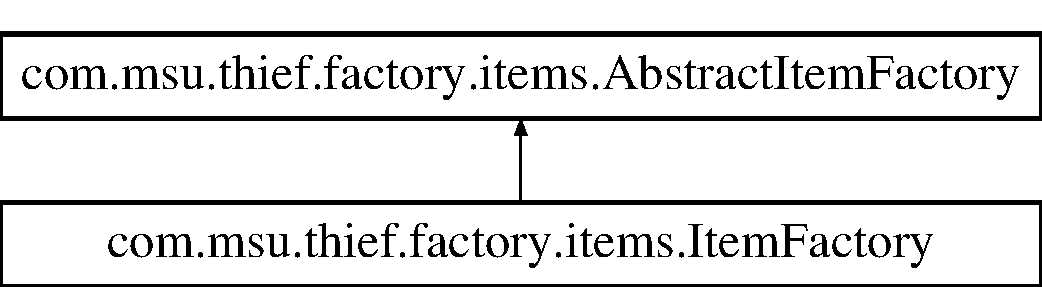
\includegraphics[height=2.000000cm]{classcom_1_1msu_1_1thief_1_1factory_1_1items_1_1AbstractItemFactory}
\end{center}
\end{figure}
\subsection*{Public Member Functions}
\begin{DoxyCompactItemize}
\item 
\hypertarget{classcom_1_1msu_1_1thief_1_1factory_1_1items_1_1AbstractItemFactory_a85d7e14b1a7d20560df88e59ef7fb259}{abstract \hyperlink{classcom_1_1msu_1_1thief_1_1model_1_1Item}{Item} {\bfseries create} ()}\label{classcom_1_1msu_1_1thief_1_1factory_1_1items_1_1AbstractItemFactory_a85d7e14b1a7d20560df88e59ef7fb259}

\item 
\hypertarget{classcom_1_1msu_1_1thief_1_1factory_1_1items_1_1AbstractItemFactory_ae831f959808ee2603e74baf311b7d4fa}{Collection$<$ \hyperlink{classcom_1_1msu_1_1thief_1_1model_1_1Item}{Item} $>$ {\bfseries create} (int n)}\label{classcom_1_1msu_1_1thief_1_1factory_1_1items_1_1AbstractItemFactory_ae831f959808ee2603e74baf311b7d4fa}

\end{DoxyCompactItemize}


\subsection{Detailed Description}
Abstract factory for creating items 

The documentation for this class was generated from the following file\-:\begin{DoxyCompactItemize}
\item 
src/main/java/com/msu/thief/factory/items/Abstract\-Item\-Factory.\-java\end{DoxyCompactItemize}

\hypertarget{classcom_1_1msu_1_1knp_1_1experiment_1_1AbstractKNPExperiment}{\section{com.\-msu.\-knp.\-experiment.\-Abstract\-K\-N\-P\-Experiment Class Reference}
\label{classcom_1_1msu_1_1knp_1_1experiment_1_1AbstractKNPExperiment}\index{com.\-msu.\-knp.\-experiment.\-Abstract\-K\-N\-P\-Experiment@{com.\-msu.\-knp.\-experiment.\-Abstract\-K\-N\-P\-Experiment}}
}
Inheritance diagram for com.\-msu.\-knp.\-experiment.\-Abstract\-K\-N\-P\-Experiment\-:\begin{figure}[H]
\begin{center}
\leavevmode
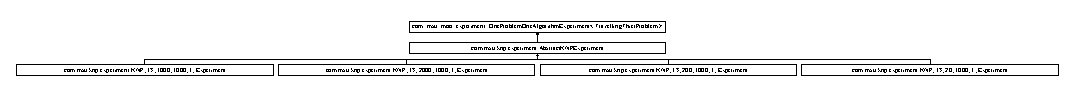
\includegraphics[height=0.783582cm]{classcom_1_1msu_1_1knp_1_1experiment_1_1AbstractKNPExperiment}
\end{center}
\end{figure}
\subsection*{Public Member Functions}
\begin{DoxyCompactItemize}
\item 
\hypertarget{classcom_1_1msu_1_1knp_1_1experiment_1_1AbstractKNPExperiment_a66c8de1695336bb9ab4a7939d5b170a8}{void {\bfseries visualize} ()}\label{classcom_1_1msu_1_1knp_1_1experiment_1_1AbstractKNPExperiment_a66c8de1695336bb9ab4a7939d5b170a8}

\end{DoxyCompactItemize}
\subsection*{Protected Member Functions}
\begin{DoxyCompactItemize}
\item 
\hypertarget{classcom_1_1msu_1_1knp_1_1experiment_1_1AbstractKNPExperiment_ab8c8ffebc97f2bfc8678c6b1ed6eb6d6}{abstract Integer\mbox{[}$\,$\mbox{]}\mbox{[}$\,$\mbox{]} {\bfseries get\-Items} ()}\label{classcom_1_1msu_1_1knp_1_1experiment_1_1AbstractKNPExperiment_ab8c8ffebc97f2bfc8678c6b1ed6eb6d6}

\item 
\hypertarget{classcom_1_1msu_1_1knp_1_1experiment_1_1AbstractKNPExperiment_accbb89d4b4f45734e2f3540fc76cc656}{abstract Integer\mbox{[}$\,$\mbox{]} {\bfseries get\-Optimum} ()}\label{classcom_1_1msu_1_1knp_1_1experiment_1_1AbstractKNPExperiment_accbb89d4b4f45734e2f3540fc76cc656}

\item 
\hypertarget{classcom_1_1msu_1_1knp_1_1experiment_1_1AbstractKNPExperiment_a208d2eaaab58f4d6f6bd397a0819d8c0}{abstract Integer {\bfseries get\-Max\-Weight} ()}\label{classcom_1_1msu_1_1knp_1_1experiment_1_1AbstractKNPExperiment_a208d2eaaab58f4d6f6bd397a0819d8c0}

\item 
\hypertarget{classcom_1_1msu_1_1knp_1_1experiment_1_1AbstractKNPExperiment_af311b9ed85d2fc1a7b01fb7a91157dca}{I\-Algorithm\\*
$<$ \hyperlink{classcom_1_1msu_1_1thief_1_1problems_1_1TravellingThiefProblem}{Travelling\-Thief\-Problem} $>$ {\bfseries get\-Algorithm} ()}\label{classcom_1_1msu_1_1knp_1_1experiment_1_1AbstractKNPExperiment_af311b9ed85d2fc1a7b01fb7a91157dca}

\item 
\hypertarget{classcom_1_1msu_1_1knp_1_1experiment_1_1AbstractKNPExperiment_a5a8de059fb862c9299f56d01259bdcfe}{\hyperlink{classcom_1_1msu_1_1thief_1_1problems_1_1TravellingThiefProblem}{Travelling\-Thief\-Problem} {\bfseries get\-Problem} ()}\label{classcom_1_1msu_1_1knp_1_1experiment_1_1AbstractKNPExperiment_a5a8de059fb862c9299f56d01259bdcfe}

\item 
\hypertarget{classcom_1_1msu_1_1knp_1_1experiment_1_1AbstractKNPExperiment_a3bfc662e5dad83990fc88a6ab526ce85}{Non\-Dominated\-Solution\-Set {\bfseries get\-True\-Front} ()}\label{classcom_1_1msu_1_1knp_1_1experiment_1_1AbstractKNPExperiment_a3bfc662e5dad83990fc88a6ab526ce85}

\end{DoxyCompactItemize}


The documentation for this class was generated from the following file\-:\begin{DoxyCompactItemize}
\item 
src/main/java/com/msu/knp/experiment/Abstract\-K\-N\-P\-Experiment.\-java\end{DoxyCompactItemize}

\hypertarget{classcom_1_1msu_1_1thief_1_1factory_1_1map_1_1AbstractMapFactory}{\section{com.\-msu.\-thief.\-factory.\-map.\-Abstract\-Map\-Factory Class Reference}
\label{classcom_1_1msu_1_1thief_1_1factory_1_1map_1_1AbstractMapFactory}\index{com.\-msu.\-thief.\-factory.\-map.\-Abstract\-Map\-Factory@{com.\-msu.\-thief.\-factory.\-map.\-Abstract\-Map\-Factory}}
}
Inheritance diagram for com.\-msu.\-thief.\-factory.\-map.\-Abstract\-Map\-Factory\-:\begin{figure}[H]
\begin{center}
\leavevmode
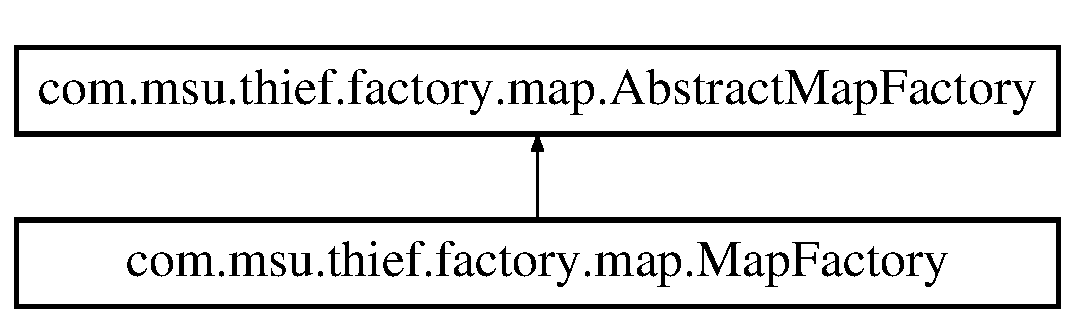
\includegraphics[height=2.000000cm]{classcom_1_1msu_1_1thief_1_1factory_1_1map_1_1AbstractMapFactory}
\end{center}
\end{figure}
\subsection*{Public Member Functions}
\begin{DoxyCompactItemize}
\item 
\hypertarget{classcom_1_1msu_1_1thief_1_1factory_1_1map_1_1AbstractMapFactory_a8d7acb0ef65995620cb558c1e3de2b3e}{abstract \hyperlink{classcom_1_1msu_1_1thief_1_1model_1_1SymmetricMap}{Symmetric\-Map} {\bfseries create} (int n)}\label{classcom_1_1msu_1_1thief_1_1factory_1_1map_1_1AbstractMapFactory_a8d7acb0ef65995620cb558c1e3de2b3e}

\end{DoxyCompactItemize}


The documentation for this class was generated from the following file\-:\begin{DoxyCompactItemize}
\item 
src/main/java/com/msu/thief/factory/map/Abstract\-Map\-Factory.\-java\end{DoxyCompactItemize}

\hypertarget{classcom_1_1msu_1_1tsp_1_1experiment_1_1AbstractTSPExperiment}{\section{com.\-msu.\-tsp.\-experiment.\-Abstract\-T\-S\-P\-Experiment Class Reference}
\label{classcom_1_1msu_1_1tsp_1_1experiment_1_1AbstractTSPExperiment}\index{com.\-msu.\-tsp.\-experiment.\-Abstract\-T\-S\-P\-Experiment@{com.\-msu.\-tsp.\-experiment.\-Abstract\-T\-S\-P\-Experiment}}
}
Inheritance diagram for com.\-msu.\-tsp.\-experiment.\-Abstract\-T\-S\-P\-Experiment\-:\begin{figure}[H]
\begin{center}
\leavevmode
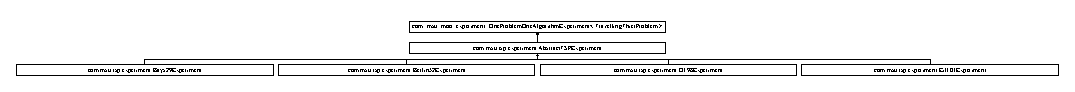
\includegraphics[height=0.783582cm]{classcom_1_1msu_1_1tsp_1_1experiment_1_1AbstractTSPExperiment}
\end{center}
\end{figure}
\subsection*{Public Member Functions}
\begin{DoxyCompactItemize}
\item 
\hypertarget{classcom_1_1msu_1_1tsp_1_1experiment_1_1AbstractTSPExperiment_a59d28e7a5d374f6773d6ce2bfc667923}{void {\bfseries report} ()}\label{classcom_1_1msu_1_1tsp_1_1experiment_1_1AbstractTSPExperiment_a59d28e7a5d374f6773d6ce2bfc667923}

\end{DoxyCompactItemize}
\subsection*{Protected Member Functions}
\begin{DoxyCompactItemize}
\item 
\hypertarget{classcom_1_1msu_1_1tsp_1_1experiment_1_1AbstractTSPExperiment_ac93a047cb36695f583c582125cd10552}{abstract double\mbox{[}$\,$\mbox{]}\mbox{[}$\,$\mbox{]} {\bfseries get\-Points} ()}\label{classcom_1_1msu_1_1tsp_1_1experiment_1_1AbstractTSPExperiment_ac93a047cb36695f583c582125cd10552}

\item 
\hypertarget{classcom_1_1msu_1_1tsp_1_1experiment_1_1AbstractTSPExperiment_aa2dbdc845df365fc345aab7192328c93}{abstract Integer\mbox{[}$\,$\mbox{]} {\bfseries get\-Optimum} ()}\label{classcom_1_1msu_1_1tsp_1_1experiment_1_1AbstractTSPExperiment_aa2dbdc845df365fc345aab7192328c93}

\item 
\hypertarget{classcom_1_1msu_1_1tsp_1_1experiment_1_1AbstractTSPExperiment_a579feb24e16e82539501353790c3c107}{I\-Algorithm\\*
$<$ \hyperlink{classcom_1_1msu_1_1thief_1_1problems_1_1TravellingThiefProblem}{Travelling\-Thief\-Problem} $>$ {\bfseries get\-Algorithm} ()}\label{classcom_1_1msu_1_1tsp_1_1experiment_1_1AbstractTSPExperiment_a579feb24e16e82539501353790c3c107}

\item 
\hypertarget{classcom_1_1msu_1_1tsp_1_1experiment_1_1AbstractTSPExperiment_a6f5c172cffcff1458591ec8d44cb8d12}{\hyperlink{classcom_1_1msu_1_1thief_1_1problems_1_1TravellingThiefProblem}{Travelling\-Thief\-Problem} {\bfseries get\-Problem} ()}\label{classcom_1_1msu_1_1tsp_1_1experiment_1_1AbstractTSPExperiment_a6f5c172cffcff1458591ec8d44cb8d12}

\item 
\hypertarget{classcom_1_1msu_1_1tsp_1_1experiment_1_1AbstractTSPExperiment_a29b30ab38b406a029bc5b7a994584543}{Non\-Dominated\-Solution\-Set {\bfseries get\-True\-Front} ()}\label{classcom_1_1msu_1_1tsp_1_1experiment_1_1AbstractTSPExperiment_a29b30ab38b406a029bc5b7a994584543}

\end{DoxyCompactItemize}


The documentation for this class was generated from the following file\-:\begin{DoxyCompactItemize}
\item 
src/main/java/com/msu/tsp/experiment/Abstract\-T\-S\-P\-Experiment.\-java\end{DoxyCompactItemize}

\hypertarget{classcom_1_1msu_1_1thief_1_1factory_1_1AlgorithmFactory}{\section{com.\-msu.\-thief.\-factory.\-Algorithm\-Factory Class Reference}
\label{classcom_1_1msu_1_1thief_1_1factory_1_1AlgorithmFactory}\index{com.\-msu.\-thief.\-factory.\-Algorithm\-Factory@{com.\-msu.\-thief.\-factory.\-Algorithm\-Factory}}
}
\subsection*{Static Public Member Functions}
\begin{DoxyCompactItemize}
\item 
\hypertarget{classcom_1_1msu_1_1thief_1_1factory_1_1AlgorithmFactory_a4c4d6046c4a77971d55af366ba2e17aa}{static N\-S\-G\-A\-I\-I$<$ \hyperlink{classcom_1_1msu_1_1thief_1_1variable_1_1TTPVariable}{T\-T\-P\-Variable}, \\*
\hyperlink{classcom_1_1msu_1_1thief_1_1problems_1_1TravellingThiefProblem}{Travelling\-Thief\-Problem} $>$ {\bfseries create\-N\-S\-G\-A\-I\-I} ()}\label{classcom_1_1msu_1_1thief_1_1factory_1_1AlgorithmFactory_a4c4d6046c4a77971d55af366ba2e17aa}

\item 
\hypertarget{classcom_1_1msu_1_1thief_1_1factory_1_1AlgorithmFactory_a5f9f71ccff99caff8addaf104f26ad91}{static N\-S\-G\-A\-I\-I\-Builder\\*
$<$ \hyperlink{classcom_1_1msu_1_1thief_1_1variable_1_1TTPVariable}{T\-T\-P\-Variable}, \\*
\hyperlink{classcom_1_1msu_1_1thief_1_1problems_1_1TravellingThiefProblem}{Travelling\-Thief\-Problem} $>$ {\bfseries create\-N\-S\-G\-A\-I\-I\-Builder} ()}\label{classcom_1_1msu_1_1thief_1_1factory_1_1AlgorithmFactory_a5f9f71ccff99caff8addaf104f26ad91}

\end{DoxyCompactItemize}


The documentation for this class was generated from the following file\-:\begin{DoxyCompactItemize}
\item 
src/main/java/com/msu/thief/factory/Algorithm\-Factory.\-java\end{DoxyCompactItemize}

\hypertarget{classcom_1_1msu_1_1thief_1_1App}{\section{com.\-msu.\-thief.\-App Class Reference}
\label{classcom_1_1msu_1_1thief_1_1App}\index{com.\-msu.\-thief.\-App@{com.\-msu.\-thief.\-App}}
}
\subsection*{Static Public Member Functions}
\begin{DoxyCompactItemize}
\item 
\hypertarget{classcom_1_1msu_1_1thief_1_1App_acbac2a1ca0853656eadc499320de6e63}{static \hyperlink{classcom_1_1msu_1_1thief_1_1problems_1_1TravellingThiefProblem}{Travelling\-Thief\-Problem} {\bfseries example} ()}\label{classcom_1_1msu_1_1thief_1_1App_acbac2a1ca0853656eadc499320de6e63}

\item 
\hypertarget{classcom_1_1msu_1_1thief_1_1App_a8ab0d5db89bc845332a0c4bb5c4e53aa}{static void {\bfseries main} (String\mbox{[}$\,$\mbox{]} args)  throws J\-M\-Exception }\label{classcom_1_1msu_1_1thief_1_1App_a8ab0d5db89bc845332a0c4bb5c4e53aa}

\end{DoxyCompactItemize}


The documentation for this class was generated from the following file\-:\begin{DoxyCompactItemize}
\item 
src/main/java/com/msu/thief/App.\-java\end{DoxyCompactItemize}

\hypertarget{classcom_1_1msu_1_1tsp_1_1experiment_1_1Bays29Experiment}{\section{com.\-msu.\-tsp.\-experiment.\-Bays29\-Experiment Class Reference}
\label{classcom_1_1msu_1_1tsp_1_1experiment_1_1Bays29Experiment}\index{com.\-msu.\-tsp.\-experiment.\-Bays29\-Experiment@{com.\-msu.\-tsp.\-experiment.\-Bays29\-Experiment}}
}
Inheritance diagram for com.\-msu.\-tsp.\-experiment.\-Bays29\-Experiment\-:\begin{figure}[H]
\begin{center}
\leavevmode
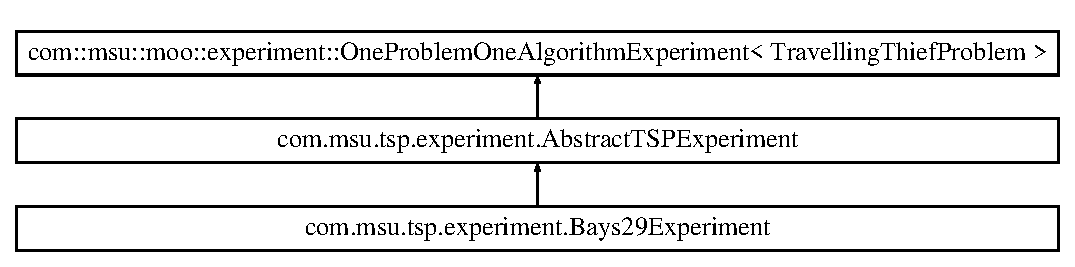
\includegraphics[height=3.000000cm]{classcom_1_1msu_1_1tsp_1_1experiment_1_1Bays29Experiment}
\end{center}
\end{figure}
\subsection*{Static Public Attributes}
\begin{DoxyCompactItemize}
\item 
\hypertarget{classcom_1_1msu_1_1tsp_1_1experiment_1_1Bays29Experiment_af4c33d5963feccff64f5e0c6b226ecc8}{static Integer\mbox{[}$\,$\mbox{]} {\bfseries O\-P\-T\-I\-M\-A\-L} = new Integer\mbox{[}$\,$\mbox{]} \{ 0, 27, 5, 11, 8, 4, 25, 28, 2, 1, 19, 9, 3, 14, 17, 16, 13, 21, 10, 18, 24, 6, 22, 26, 7, 23, 15, 12, 20 \}}\label{classcom_1_1msu_1_1tsp_1_1experiment_1_1Bays29Experiment_af4c33d5963feccff64f5e0c6b226ecc8}

\item 
static double\mbox{[}$\,$\mbox{]}\mbox{[}$\,$\mbox{]} {\bfseries M\-A\-P}
\end{DoxyCompactItemize}
\subsection*{Protected Member Functions}
\begin{DoxyCompactItemize}
\item 
\hypertarget{classcom_1_1msu_1_1tsp_1_1experiment_1_1Bays29Experiment_af0bd8b40e641901b5b1a916ac3fd0a2d}{double\mbox{[}$\,$\mbox{]}\mbox{[}$\,$\mbox{]} {\bfseries get\-Points} ()}\label{classcom_1_1msu_1_1tsp_1_1experiment_1_1Bays29Experiment_af0bd8b40e641901b5b1a916ac3fd0a2d}

\item 
\hypertarget{classcom_1_1msu_1_1tsp_1_1experiment_1_1Bays29Experiment_a0c84bb2d195c704bc837fed2b9acdbf2}{Integer\mbox{[}$\,$\mbox{]} {\bfseries get\-Optimum} ()}\label{classcom_1_1msu_1_1tsp_1_1experiment_1_1Bays29Experiment_a0c84bb2d195c704bc837fed2b9acdbf2}

\end{DoxyCompactItemize}
\subsection*{Additional Inherited Members}


\subsection{Member Data Documentation}
\hypertarget{classcom_1_1msu_1_1tsp_1_1experiment_1_1Bays29Experiment_a8add5b3b067a46f8159ac14683ad9930}{\index{com\-::msu\-::tsp\-::experiment\-::\-Bays29\-Experiment@{com\-::msu\-::tsp\-::experiment\-::\-Bays29\-Experiment}!M\-A\-P@{M\-A\-P}}
\index{M\-A\-P@{M\-A\-P}!com::msu::tsp::experiment::Bays29Experiment@{com\-::msu\-::tsp\-::experiment\-::\-Bays29\-Experiment}}
\subsubsection[{M\-A\-P}]{\setlength{\rightskip}{0pt plus 5cm}double \mbox{[}$\,$\mbox{]}\mbox{[}$\,$\mbox{]} com.\-msu.\-tsp.\-experiment.\-Bays29\-Experiment.\-M\-A\-P\hspace{0.3cm}{\ttfamily [static]}}}\label{classcom_1_1msu_1_1tsp_1_1experiment_1_1Bays29Experiment_a8add5b3b067a46f8159ac14683ad9930}
{\bfseries Initial value\-:}
\begin{DoxyCode}
= \textcolor{keyword}{new} \textcolor{keywordtype}{double}[][] \{
            \{ 0, 107, 241, 190, 124, 80, 316, 76, 152, 157, 283, 133, 113, 297, 228, 129, 348, 276, 188, 
      150, 65, 341, 184, 67, 221, 169, 108, 45, 167 \},
            \{ 107, 0, 148, 137, 88, 127, 336, 183, 134, 95, 254, 180, 101, 234, 175, 176, 265, 199, 182, 67
      , 42, 278, 271, 146, 251, 105, 191, 139, 79 \},
            \{ 241, 148, 0, 374, 171, 259, 509, 317, 217, 232, 491, 312, 280, 391, 412, 349, 422, 356, 355, 
      204, 182, 435, 417, 292, 424, 116, 337, 273, 77 \},
            \{ 190, 137, 374, 0, 202, 234, 222, 192, 248, 42, 117, 287, 79, 107, 38, 121, 152, 86, 68, 70, 
      137, 151, 239, 135, 137, 242, 165, 228, 205 \},
            \{ 124, 88, 171, 202, 0, 61, 392, 202, 46, 160, 319, 112, 163, 322, 240, 232, 314, 287, 238, 155
      , 65, 366, 300, 175, 307, 57, 220, 121, 97 \},
            \{ 80, 127, 259, 234, 61, 0, 386, 141, 72, 167, 351, 55, 157, 331, 272, 226, 362, 296, 232, 164,
       85, 375, 249, 147, 301, 118, 188, 60, 185 \},
            \{ 316, 336, 509, 222, 392, 386, 0, 233, 438, 254, 202, 439, 235, 254, 210, 187, 313, 266, 154, 
      282, 321, 298, 168, 249, 95, 437, 190, 314, 435 \},
            \{ 76, 183, 317, 192, 202, 141, 233, 0, 213, 188, 272, 193, 131, 302, 233, 98, 344, 289, 177, 
      216, 141, 346, 108, 57, 190, 245, 43, 81, 243 \},
            \{ 152, 134, 217, 248, 46, 72, 438, 213, 0, 206, 365, 89, 209, 368, 286, 278, 360, 333, 284, 201
      , 111, 412, 321, 221, 353, 72, 266, 132, 111 \},
            \{ 157, 95, 232, 42, 160, 167, 254, 188, 206, 0, 159, 220, 57, 149, 80, 132, 193, 127, 100, 28, 
      95, 193, 241, 131, 169, 200, 161, 189, 163 \},
            \{ 283, 254, 491, 117, 319, 351, 202, 272, 365, 159, 0, 404, 176, 106, 79, 161, 165, 141, 95, 
      187, 254, 103, 279, 215, 117, 359, 216, 308, 322 \},
            \{ 133, 180, 312, 287, 112, 55, 439, 193, 89, 220, 404, 0, 210, 384, 325, 279, 415, 349, 285, 
      217, 138, 428, 310, 200, 354, 169, 241, 112, 238 \},
            \{ 113, 101, 280, 79, 163, 157, 235, 131, 209, 57, 176, 210, 0, 186, 117, 75, 231, 165, 81, 85, 
      92, 230, 184, 74, 150, 208, 104, 158, 206 \},
            \{ 297, 234, 391, 107, 322, 331, 254, 302, 368, 149, 106, 384, 186, 0, 69, 191, 59, 35, 125, 167
      , 255, 44, 309, 245, 169, 327, 246, 335, 288 \},
            \{ 228, 175, 412, 38, 240, 272, 210, 233, 286, 80, 79, 325, 117, 69, 0, 122, 122, 56, 56, 108, 
      175, 113, 240, 176, 125, 280, 177, 266, 243 \},
            \{ 129, 176, 349, 121, 232, 226, 187, 98, 278, 132, 161, 279, 75, 191, 122, 0, 244, 178, 66, 160
      , 161, 235, 118, 62, 92, 277, 55, 155, 275 \},
            \{ 348, 265, 422, 152, 314, 362, 313, 344, 360, 193, 165, 415, 231, 59, 122, 244, 0, 66, 178, 
      198, 286, 77, 362, 287, 228, 358, 299, 380, 319 \},
            \{ 276, 199, 356, 86, 287, 296, 266, 289, 333, 127, 141, 349, 165, 35, 56, 178, 66, 0, 112, 132,
       220, 79, 296, 232, 181, 292, 233, 314, 253 \},
            \{ 188, 182, 355, 68, 238, 232, 154, 177, 284, 100, 95, 285, 81, 125, 56, 66, 178, 112, 0, 128, 
      167, 169, 179, 120, 69, 283, 121, 213, 281 \},
            \{ 150, 67, 204, 70, 155, 164, 282, 216, 201, 28, 187, 217, 85, 167, 108, 160, 198, 132, 128, 0,
       88, 211, 269, 159, 197, 172, 189, 182, 135 \},
            \{ 65, 42, 182, 137, 65, 85, 321, 141, 111, 95, 254, 138, 92, 255, 175, 161, 286, 220, 167, 88, 
      0, 299, 229, 104, 236, 110, 149, 97, 108 \},
            \{ 341, 278, 435, 151, 366, 375, 298, 346, 412, 193, 103, 428, 230, 44, 113, 235, 77, 79, 169, 
      211, 299, 0, 353, 289, 213, 371, 290, 379, 332 \},
            \{ 184, 271, 417, 239, 300, 249, 168, 108, 321, 241, 279, 310, 184, 309, 240, 118, 362, 296, 179
      , 269, 229, 353, 0, 121, 162, 345, 80, 189, 342 \},
            \{ 67, 146, 292, 135, 175, 147, 249, 57, 221, 131, 215, 200, 74, 245, 176, 62, 287, 232, 120, 
      159, 104, 289, 121, 0, 154, 220, 41, 93, 218 \},
            \{ 221, 251, 424, 137, 307, 301, 95, 190, 353, 169, 117, 354, 150, 169, 125, 92, 228, 181, 69, 
      197, 236, 213, 162, 154, 0, 352, 147, 247, 350 \},
            \{ 169, 105, 116, 242, 57, 118, 437, 245, 72, 200, 359, 169, 208, 327, 280, 277, 358, 292, 283, 
      172, 110, 371, 345, 220, 352, 0, 265, 178, 39 \},
            \{ 108, 191, 337, 165, 220, 188, 190, 43, 266, 161, 216, 241, 104, 246, 177, 55, 299, 233, 121, 
      189, 149, 290, 80, 41, 147, 265, 0, 124, 263 \},
            \{ 45, 139, 273, 228, 121, 60, 314, 81, 132, 189, 308, 112, 158, 335, 266, 155, 380, 314, 213, 
      182, 97, 379, 189, 93, 247, 178, 124, 0, 199 \},
            \{ 167, 79, 77, 205, 97, 185, 435, 243, 111, 163, 322, 238, 206, 288, 243, 275, 319, 253, 281, 
      135, 108, 332, 342, 218, 350, 39, 263, 199, 0 \} \}
\end{DoxyCode}


The documentation for this class was generated from the following file\-:\begin{DoxyCompactItemize}
\item 
src/main/java/com/msu/tsp/experiment/Bays29\-Experiment.\-java\end{DoxyCompactItemize}

\hypertarget{classcom_1_1msu_1_1tsp_1_1experiment_1_1Berlin52Experiment}{\section{com.\-msu.\-tsp.\-experiment.\-Berlin52\-Experiment Class Reference}
\label{classcom_1_1msu_1_1tsp_1_1experiment_1_1Berlin52Experiment}\index{com.\-msu.\-tsp.\-experiment.\-Berlin52\-Experiment@{com.\-msu.\-tsp.\-experiment.\-Berlin52\-Experiment}}
}
Inheritance diagram for com.\-msu.\-tsp.\-experiment.\-Berlin52\-Experiment\-:\begin{figure}[H]
\begin{center}
\leavevmode
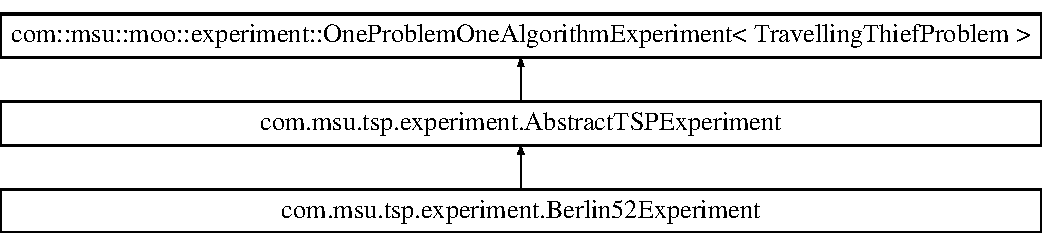
\includegraphics[height=3.000000cm]{classcom_1_1msu_1_1tsp_1_1experiment_1_1Berlin52Experiment}
\end{center}
\end{figure}
\subsection*{Protected Member Functions}
\begin{DoxyCompactItemize}
\item 
\hypertarget{classcom_1_1msu_1_1tsp_1_1experiment_1_1Berlin52Experiment_a5149fdd1771427ccb5817e40ecd9f389}{double\mbox{[}$\,$\mbox{]}\mbox{[}$\,$\mbox{]} {\bfseries get\-Points} ()}\label{classcom_1_1msu_1_1tsp_1_1experiment_1_1Berlin52Experiment_a5149fdd1771427ccb5817e40ecd9f389}

\item 
\hypertarget{classcom_1_1msu_1_1tsp_1_1experiment_1_1Berlin52Experiment_af52644a24c2e905a93e64077090cf448}{Integer\mbox{[}$\,$\mbox{]} {\bfseries get\-Optimum} ()}\label{classcom_1_1msu_1_1tsp_1_1experiment_1_1Berlin52Experiment_af52644a24c2e905a93e64077090cf448}

\end{DoxyCompactItemize}
\subsection*{Additional Inherited Members}


The documentation for this class was generated from the following file\-:\begin{DoxyCompactItemize}
\item 
src/main/java/com/msu/tsp/experiment/Berlin52\-Experiment.\-java\end{DoxyCompactItemize}

\hypertarget{classcom_1_1msu_1_1thief_1_1experiment_1_1BonyadiExperiment}{\section{com.\-msu.\-thief.\-experiment.\-Bonyadi\-Experiment Class Reference}
\label{classcom_1_1msu_1_1thief_1_1experiment_1_1BonyadiExperiment}\index{com.\-msu.\-thief.\-experiment.\-Bonyadi\-Experiment@{com.\-msu.\-thief.\-experiment.\-Bonyadi\-Experiment}}
}
Inheritance diagram for com.\-msu.\-thief.\-experiment.\-Bonyadi\-Experiment\-:\begin{figure}[H]
\begin{center}
\leavevmode
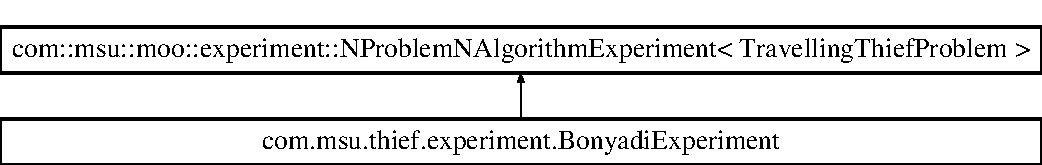
\includegraphics[height=2.000000cm]{classcom_1_1msu_1_1thief_1_1experiment_1_1BonyadiExperiment}
\end{center}
\end{figure}
\subsection*{Static Public Attributes}
\begin{DoxyCompactItemize}
\item 
final static String\mbox{[}$\,$\mbox{]} {\bfseries I\-N\-S\-T\-A\-N\-C\-E\-S}
\end{DoxyCompactItemize}
\subsection*{Protected Member Functions}
\begin{DoxyCompactItemize}
\item 
\hypertarget{classcom_1_1msu_1_1thief_1_1experiment_1_1BonyadiExperiment_a1a589a4c2c4d1339dea4ac5dbbd71503}{List$<$ I\-Algorithm\\*
$<$ \hyperlink{classcom_1_1msu_1_1thief_1_1problems_1_1TravellingThiefProblem}{Travelling\-Thief\-Problem} $>$ $>$ {\bfseries get\-Algorithms} ()}\label{classcom_1_1msu_1_1thief_1_1experiment_1_1BonyadiExperiment_a1a589a4c2c4d1339dea4ac5dbbd71503}

\item 
\hypertarget{classcom_1_1msu_1_1thief_1_1experiment_1_1BonyadiExperiment_a2550205e73a7969136ed1e022b633685}{Map$<$ \hyperlink{classcom_1_1msu_1_1thief_1_1problems_1_1TravellingThiefProblem}{Travelling\-Thief\-Problem}, \\*
Non\-Dominated\-Solution\-Set $>$ {\bfseries get\-Problems} ()}\label{classcom_1_1msu_1_1thief_1_1experiment_1_1BonyadiExperiment_a2550205e73a7969136ed1e022b633685}

\end{DoxyCompactItemize}


\subsection{Member Data Documentation}
\hypertarget{classcom_1_1msu_1_1thief_1_1experiment_1_1BonyadiExperiment_a6713640646f3d6dc1d9991afc8bf1190}{\index{com\-::msu\-::thief\-::experiment\-::\-Bonyadi\-Experiment@{com\-::msu\-::thief\-::experiment\-::\-Bonyadi\-Experiment}!I\-N\-S\-T\-A\-N\-C\-E\-S@{I\-N\-S\-T\-A\-N\-C\-E\-S}}
\index{I\-N\-S\-T\-A\-N\-C\-E\-S@{I\-N\-S\-T\-A\-N\-C\-E\-S}!com::msu::thief::experiment::BonyadiExperiment@{com\-::msu\-::thief\-::experiment\-::\-Bonyadi\-Experiment}}
\subsubsection[{I\-N\-S\-T\-A\-N\-C\-E\-S}]{\setlength{\rightskip}{0pt plus 5cm}final static String \mbox{[}$\,$\mbox{]} com.\-msu.\-thief.\-experiment.\-Bonyadi\-Experiment.\-I\-N\-S\-T\-A\-N\-C\-E\-S\hspace{0.3cm}{\ttfamily [static]}}}\label{classcom_1_1msu_1_1thief_1_1experiment_1_1BonyadiExperiment_a6713640646f3d6dc1d9991afc8bf1190}
{\bfseries Initial value\-:}
\begin{DoxyCode}
= \textcolor{keyword}{new} String[] \{ 
            \textcolor{stringliteral}{"../ttp-benchmark/10/10\_15\_10\_75.txt"},
            \textcolor{stringliteral}{"../ttp-benchmark/20/20\_25\_10\_75.txt"},
            \textcolor{stringliteral}{"../ttp-benchmark/50/50\_75\_10\_75.txt"},
            \textcolor{stringliteral}{"../ttp-benchmark/100/100\_150\_10\_75.txt"},
    \}
\end{DoxyCode}


The documentation for this class was generated from the following file\-:\begin{DoxyCompactItemize}
\item 
src/main/java/com/msu/thief/experiment/Bonyadi\-Experiment.\-java\end{DoxyCompactItemize}

\hypertarget{classcom_1_1msu_1_1thief_1_1factory_1_1BonyadiFactory}{\section{com.\-msu.\-thief.\-factory.\-Bonyadi\-Factory Class Reference}
\label{classcom_1_1msu_1_1thief_1_1factory_1_1BonyadiFactory}\index{com.\-msu.\-thief.\-factory.\-Bonyadi\-Factory@{com.\-msu.\-thief.\-factory.\-Bonyadi\-Factory}}
}
\subsection*{Public Member Functions}
\begin{DoxyCompactItemize}
\item 
\hypertarget{classcom_1_1msu_1_1thief_1_1factory_1_1BonyadiFactory_aba39f47d8b90379dfddc7b9877674ba1}{\hyperlink{classcom_1_1msu_1_1thief_1_1problems_1_1TravellingThiefProblem}{Travelling\-Thief\-Problem} {\bfseries create} (String path\-To\-File)}\label{classcom_1_1msu_1_1thief_1_1factory_1_1BonyadiFactory_aba39f47d8b90379dfddc7b9877674ba1}

\end{DoxyCompactItemize}


The documentation for this class was generated from the following file\-:\begin{DoxyCompactItemize}
\item 
src/main/java/com/msu/thief/factory/Bonyadi\-Factory.\-java\end{DoxyCompactItemize}

\hypertarget{classcom_1_1msu_1_1thief_1_1factory_1_1BonyadiFactoryModel1}{\section{com.\-msu.\-thief.\-factory.\-Bonyadi\-Factory\-Model1 Class Reference}
\label{classcom_1_1msu_1_1thief_1_1factory_1_1BonyadiFactoryModel1}\index{com.\-msu.\-thief.\-factory.\-Bonyadi\-Factory\-Model1@{com.\-msu.\-thief.\-factory.\-Bonyadi\-Factory\-Model1}}
}
\subsection*{Public Member Functions}
\begin{DoxyCompactItemize}
\item 
\hypertarget{classcom_1_1msu_1_1thief_1_1factory_1_1BonyadiFactoryModel1_a8d1d4c79661995bcf2b4a38dd0b700d0}{\hyperlink{classcom_1_1msu_1_1thief_1_1problems_1_1TravellingThiefProblem}{Travelling\-Thief\-Problem} {\bfseries create} (String path\-To\-File)}\label{classcom_1_1msu_1_1thief_1_1factory_1_1BonyadiFactoryModel1_a8d1d4c79661995bcf2b4a38dd0b700d0}

\end{DoxyCompactItemize}


The documentation for this class was generated from the following file\-:\begin{DoxyCompactItemize}
\item 
src/main/java/com/msu/thief/factory/Bonyadi\-Factory\-Model1.\-java\end{DoxyCompactItemize}

\hypertarget{classcom_1_1msu_1_1thief_1_1model_1_1packing_1_1BooleanPackingList}{\section{com.\-msu.\-thief.\-model.\-packing.\-Boolean\-Packing\-List Class Reference}
\label{classcom_1_1msu_1_1thief_1_1model_1_1packing_1_1BooleanPackingList}\index{com.\-msu.\-thief.\-model.\-packing.\-Boolean\-Packing\-List@{com.\-msu.\-thief.\-model.\-packing.\-Boolean\-Packing\-List}}
}
Inheritance diagram for com.\-msu.\-thief.\-model.\-packing.\-Boolean\-Packing\-List\-:\begin{figure}[H]
\begin{center}
\leavevmode
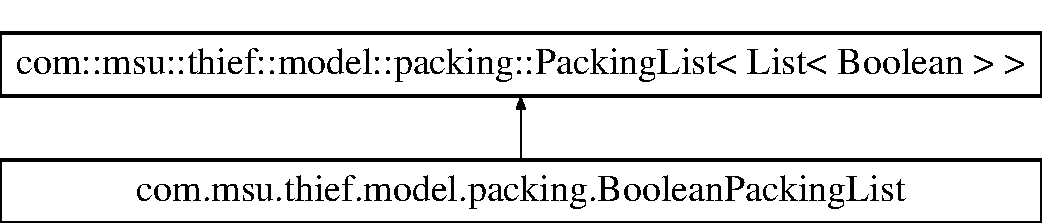
\includegraphics[height=2.000000cm]{classcom_1_1msu_1_1thief_1_1model_1_1packing_1_1BooleanPackingList}
\end{center}
\end{figure}
\subsection*{Public Member Functions}
\begin{DoxyCompactItemize}
\item 
\hypertarget{classcom_1_1msu_1_1thief_1_1model_1_1packing_1_1BooleanPackingList_ab42916643e82ce81081a8509b610c04a}{{\bfseries Boolean\-Packing\-List} (List$<$ Boolean $>$ l)}\label{classcom_1_1msu_1_1thief_1_1model_1_1packing_1_1BooleanPackingList_ab42916643e82ce81081a8509b610c04a}

\item 
\hypertarget{classcom_1_1msu_1_1thief_1_1model_1_1packing_1_1BooleanPackingList_a2e563518fca44da6cf9b5a93ff4477c0}{Packing\-List$<$ List$<$ Boolean $>$ $>$ {\bfseries copy} ()}\label{classcom_1_1msu_1_1thief_1_1model_1_1packing_1_1BooleanPackingList_a2e563518fca44da6cf9b5a93ff4477c0}

\item 
\hypertarget{classcom_1_1msu_1_1thief_1_1model_1_1packing_1_1BooleanPackingList_a9e39b760237b78f02100fcf7fe6ccfda}{List$<$ Boolean $>$ {\bfseries encode} ()}\label{classcom_1_1msu_1_1thief_1_1model_1_1packing_1_1BooleanPackingList_a9e39b760237b78f02100fcf7fe6ccfda}

\end{DoxyCompactItemize}


The documentation for this class was generated from the following file\-:\begin{DoxyCompactItemize}
\item 
src/main/java/com/msu/thief/model/packing/Boolean\-Packing\-List.\-java\end{DoxyCompactItemize}

\hypertarget{classcom_1_1msu_1_1thief_1_1model_1_1packing_1_1BooleanPackingListFactory}{\section{com.\-msu.\-thief.\-model.\-packing.\-Boolean\-Packing\-List\-Factory Class Reference}
\label{classcom_1_1msu_1_1thief_1_1model_1_1packing_1_1BooleanPackingListFactory}\index{com.\-msu.\-thief.\-model.\-packing.\-Boolean\-Packing\-List\-Factory@{com.\-msu.\-thief.\-model.\-packing.\-Boolean\-Packing\-List\-Factory}}
}
Inheritance diagram for com.\-msu.\-thief.\-model.\-packing.\-Boolean\-Packing\-List\-Factory\-:\begin{figure}[H]
\begin{center}
\leavevmode
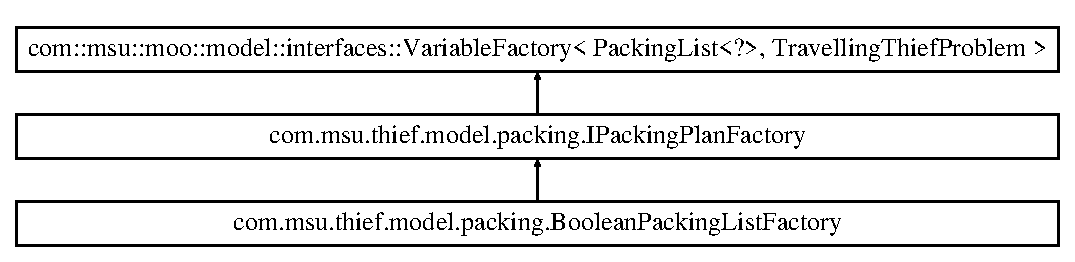
\includegraphics[height=3.000000cm]{classcom_1_1msu_1_1thief_1_1model_1_1packing_1_1BooleanPackingListFactory}
\end{center}
\end{figure}
\subsection*{Public Member Functions}
\begin{DoxyCompactItemize}
\item 
\hypertarget{classcom_1_1msu_1_1thief_1_1model_1_1packing_1_1BooleanPackingListFactory_ae8541200733c2198219f0d83d20a0f14}{Packing\-List$<$?$>$ {\bfseries create} (\hyperlink{classcom_1_1msu_1_1thief_1_1problems_1_1TravellingThiefProblem}{Travelling\-Thief\-Problem} p)}\label{classcom_1_1msu_1_1thief_1_1model_1_1packing_1_1BooleanPackingListFactory_ae8541200733c2198219f0d83d20a0f14}

\end{DoxyCompactItemize}


The documentation for this class was generated from the following file\-:\begin{DoxyCompactItemize}
\item 
src/main/java/com/msu/thief/model/packing/Boolean\-Packing\-List\-Factory.\-java\end{DoxyCompactItemize}

\hypertarget{classcom_1_1msu_1_1thief_1_1visualize_1_1ColoredTourScatterPlot}{\section{com.\-msu.\-thief.\-visualize.\-Colored\-Tour\-Scatter\-Plot Class Reference}
\label{classcom_1_1msu_1_1thief_1_1visualize_1_1ColoredTourScatterPlot}\index{com.\-msu.\-thief.\-visualize.\-Colored\-Tour\-Scatter\-Plot@{com.\-msu.\-thief.\-visualize.\-Colored\-Tour\-Scatter\-Plot}}
}
Inheritance diagram for com.\-msu.\-thief.\-visualize.\-Colored\-Tour\-Scatter\-Plot\-:\begin{figure}[H]
\begin{center}
\leavevmode
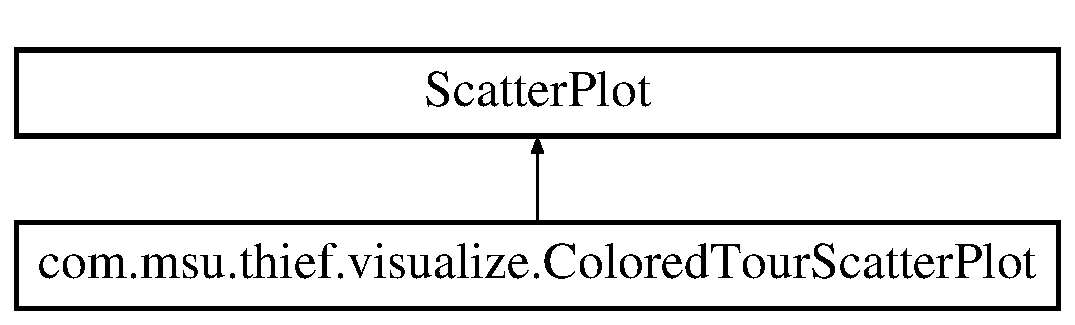
\includegraphics[height=2.000000cm]{classcom_1_1msu_1_1thief_1_1visualize_1_1ColoredTourScatterPlot}
\end{center}
\end{figure}
\subsection*{Public Member Functions}
\begin{DoxyCompactItemize}
\item 
\hypertarget{classcom_1_1msu_1_1thief_1_1visualize_1_1ColoredTourScatterPlot_a96e5d16e37eb0c860226bd69c777c712}{{\bfseries Colored\-Tour\-Scatter\-Plot} (String title)}\label{classcom_1_1msu_1_1thief_1_1visualize_1_1ColoredTourScatterPlot_a96e5d16e37eb0c860226bd69c777c712}

\item 
\hypertarget{classcom_1_1msu_1_1thief_1_1visualize_1_1ColoredTourScatterPlot_ae32ec9970c2ac9302f039a611dc6a878}{void {\bfseries add} (Solution\-Set set)}\label{classcom_1_1msu_1_1thief_1_1visualize_1_1ColoredTourScatterPlot_ae32ec9970c2ac9302f039a611dc6a878}

\item 
\hypertarget{classcom_1_1msu_1_1thief_1_1visualize_1_1ColoredTourScatterPlot_ae64b34b087ca7941cbb377da02f80fd3}{void {\bfseries add} (Solution\-Set set, String prefix)}\label{classcom_1_1msu_1_1thief_1_1visualize_1_1ColoredTourScatterPlot_ae64b34b087ca7941cbb377da02f80fd3}

\item 
\hypertarget{classcom_1_1msu_1_1thief_1_1visualize_1_1ColoredTourScatterPlot_a21e0aef1285bc91ed1f406b5c3394f75}{boolean {\bfseries is\-Show\-Labels} ()}\label{classcom_1_1msu_1_1thief_1_1visualize_1_1ColoredTourScatterPlot_a21e0aef1285bc91ed1f406b5c3394f75}

\item 
\hypertarget{classcom_1_1msu_1_1thief_1_1visualize_1_1ColoredTourScatterPlot_a6ce3e91bac3eecfb3605ad308ae5e9ee}{void {\bfseries set\-Show\-Labels} (boolean show\-Labels)}\label{classcom_1_1msu_1_1thief_1_1visualize_1_1ColoredTourScatterPlot_a6ce3e91bac3eecfb3605ad308ae5e9ee}

\end{DoxyCompactItemize}
\subsection*{Protected Attributes}
\begin{DoxyCompactItemize}
\item 
\hypertarget{classcom_1_1msu_1_1thief_1_1visualize_1_1ColoredTourScatterPlot_a1fd8f917b7e756f90aa505a578bae153}{boolean {\bfseries show\-Labels} = true}\label{classcom_1_1msu_1_1thief_1_1visualize_1_1ColoredTourScatterPlot_a1fd8f917b7e756f90aa505a578bae153}

\end{DoxyCompactItemize}


The documentation for this class was generated from the following file\-:\begin{DoxyCompactItemize}
\item 
src/main/java/com/msu/thief/visualize/Colored\-Tour\-Scatter\-Plot.\-java\end{DoxyCompactItemize}

\hypertarget{classcom_1_1msu_1_1thief_1_1util_1_1Combination}{\section{com.\-msu.\-thief.\-util.\-Combination Class Reference}
\label{classcom_1_1msu_1_1thief_1_1util_1_1Combination}\index{com.\-msu.\-thief.\-util.\-Combination@{com.\-msu.\-thief.\-util.\-Combination}}
}
\subsection*{Public Member Functions}
\begin{DoxyCompactItemize}
\item 
\hypertarget{classcom_1_1msu_1_1thief_1_1util_1_1Combination_a285d340db5caf6d5a81c0feeac737904}{{\bfseries Combination} (int n, int r)}\label{classcom_1_1msu_1_1thief_1_1util_1_1Combination_a285d340db5caf6d5a81c0feeac737904}

\item 
\hypertarget{classcom_1_1msu_1_1thief_1_1util_1_1Combination_a19d0c00f8aaf5b9b0cf535f5182f4aca}{boolean {\bfseries has\-Next} ()}\label{classcom_1_1msu_1_1thief_1_1util_1_1Combination_a19d0c00f8aaf5b9b0cf535f5182f4aca}

\item 
\hypertarget{classcom_1_1msu_1_1thief_1_1util_1_1Combination_a5637251e7695551c555fa67c1b1241be}{int\mbox{[}$\,$\mbox{]} {\bfseries next} ()}\label{classcom_1_1msu_1_1thief_1_1util_1_1Combination_a5637251e7695551c555fa67c1b1241be}

\end{DoxyCompactItemize}


The documentation for this class was generated from the following file\-:\begin{DoxyCompactItemize}
\item 
src/main/java/com/msu/thief/util/Combination.\-java\end{DoxyCompactItemize}

\hypertarget{classcom_1_1msu_1_1thief_1_1util_1_1CombinatorialUtil}{\section{com.\-msu.\-thief.\-util.\-Combinatorial\-Util Class Reference}
\label{classcom_1_1msu_1_1thief_1_1util_1_1CombinatorialUtil}\index{com.\-msu.\-thief.\-util.\-Combinatorial\-Util@{com.\-msu.\-thief.\-util.\-Combinatorial\-Util}}
}
\subsection*{Static Public Member Functions}
\begin{DoxyCompactItemize}
\item 
static$<$ T $>$ Collection$<$ List$<$ T $>$ $>$ \hyperlink{classcom_1_1msu_1_1thief_1_1util_1_1CombinatorialUtil_abb8c0a69ad77625482b17a2d14a02242}{permute} (Collection$<$ T $>$ input)
\item 
\hypertarget{classcom_1_1msu_1_1thief_1_1util_1_1CombinatorialUtil_a55d55532099946ab2b76d8e2d810be14}{static$<$ T $>$ Collection$<$ List\\*
$<$ Boolean $>$ $>$ {\bfseries get\-All\-Boolean\-Combinations} (int n)}\label{classcom_1_1msu_1_1thief_1_1util_1_1CombinatorialUtil_a55d55532099946ab2b76d8e2d810be14}

\end{DoxyCompactItemize}


\subsection{Member Function Documentation}
\hypertarget{classcom_1_1msu_1_1thief_1_1util_1_1CombinatorialUtil_abb8c0a69ad77625482b17a2d14a02242}{\index{com\-::msu\-::thief\-::util\-::\-Combinatorial\-Util@{com\-::msu\-::thief\-::util\-::\-Combinatorial\-Util}!permute@{permute}}
\index{permute@{permute}!com::msu::thief::util::CombinatorialUtil@{com\-::msu\-::thief\-::util\-::\-Combinatorial\-Util}}
\subsubsection[{permute}]{\setlength{\rightskip}{0pt plus 5cm}static $<$T$>$ Collection$<$List$<$T$>$ $>$ com.\-msu.\-thief.\-util.\-Combinatorial\-Util.\-permute (
\begin{DoxyParamCaption}
\item[{Collection$<$ T $>$}]{input}
\end{DoxyParamCaption}
)\hspace{0.3cm}{\ttfamily [inline]}, {\ttfamily [static]}}}\label{classcom_1_1msu_1_1thief_1_1util_1_1CombinatorialUtil_abb8c0a69ad77625482b17a2d14a02242}
Create all the possible permutations that exist 

The documentation for this class was generated from the following file\-:\begin{DoxyCompactItemize}
\item 
src/main/java/com/msu/thief/util/Combinatorial\-Util.\-java\end{DoxyCompactItemize}

\hypertarget{classcom_1_1msu_1_1tsp_1_1experiment_1_1D198Experiment}{\section{com.\-msu.\-tsp.\-experiment.\-D198\-Experiment Class Reference}
\label{classcom_1_1msu_1_1tsp_1_1experiment_1_1D198Experiment}\index{com.\-msu.\-tsp.\-experiment.\-D198\-Experiment@{com.\-msu.\-tsp.\-experiment.\-D198\-Experiment}}
}
Inheritance diagram for com.\-msu.\-tsp.\-experiment.\-D198\-Experiment\-:\begin{figure}[H]
\begin{center}
\leavevmode
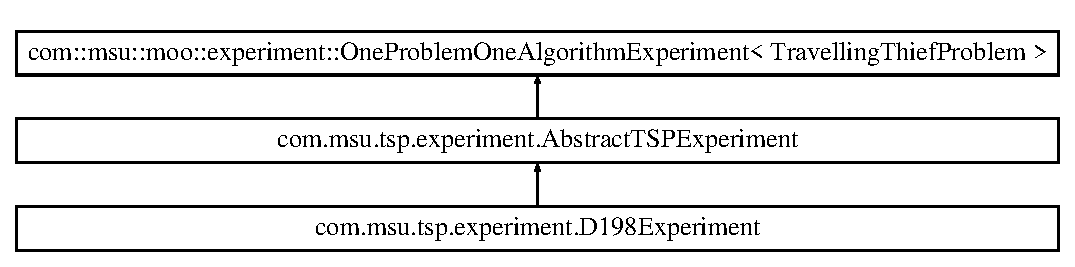
\includegraphics[height=3.000000cm]{classcom_1_1msu_1_1tsp_1_1experiment_1_1D198Experiment}
\end{center}
\end{figure}
\subsection*{Protected Member Functions}
\begin{DoxyCompactItemize}
\item 
\hypertarget{classcom_1_1msu_1_1tsp_1_1experiment_1_1D198Experiment_a29aad59f39ff13b70449bf053a6e6ab6}{double\mbox{[}$\,$\mbox{]}\mbox{[}$\,$\mbox{]} {\bfseries get\-Points} ()}\label{classcom_1_1msu_1_1tsp_1_1experiment_1_1D198Experiment_a29aad59f39ff13b70449bf053a6e6ab6}

\item 
\hypertarget{classcom_1_1msu_1_1tsp_1_1experiment_1_1D198Experiment_af4a38a000971d7caf8b97dcd954da2b5}{Integer\mbox{[}$\,$\mbox{]} {\bfseries get\-Optimum} ()}\label{classcom_1_1msu_1_1tsp_1_1experiment_1_1D198Experiment_af4a38a000971d7caf8b97dcd954da2b5}

\end{DoxyCompactItemize}
\subsection*{Additional Inherited Members}


The documentation for this class was generated from the following file\-:\begin{DoxyCompactItemize}
\item 
src/main/java/com/msu/tsp/experiment/D198\-Experiment.\-java\end{DoxyCompactItemize}

\hypertarget{classcom_1_1msu_1_1tsp_1_1experiment_1_1Eil101Experiment}{\section{com.\-msu.\-tsp.\-experiment.\-Eil101\-Experiment Class Reference}
\label{classcom_1_1msu_1_1tsp_1_1experiment_1_1Eil101Experiment}\index{com.\-msu.\-tsp.\-experiment.\-Eil101\-Experiment@{com.\-msu.\-tsp.\-experiment.\-Eil101\-Experiment}}
}
Inheritance diagram for com.\-msu.\-tsp.\-experiment.\-Eil101\-Experiment\-:\begin{figure}[H]
\begin{center}
\leavevmode
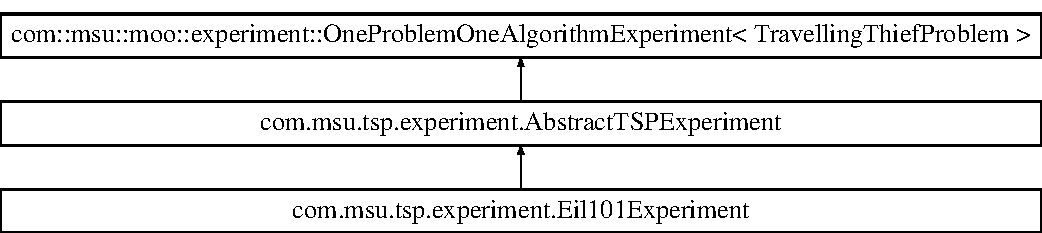
\includegraphics[height=3.000000cm]{classcom_1_1msu_1_1tsp_1_1experiment_1_1Eil101Experiment}
\end{center}
\end{figure}
\subsection*{Protected Member Functions}
\begin{DoxyCompactItemize}
\item 
\hypertarget{classcom_1_1msu_1_1tsp_1_1experiment_1_1Eil101Experiment_a50b38827fb85b4c9332c0c9fb2461dd6}{double\mbox{[}$\,$\mbox{]}\mbox{[}$\,$\mbox{]} {\bfseries get\-Points} ()}\label{classcom_1_1msu_1_1tsp_1_1experiment_1_1Eil101Experiment_a50b38827fb85b4c9332c0c9fb2461dd6}

\item 
\hypertarget{classcom_1_1msu_1_1tsp_1_1experiment_1_1Eil101Experiment_af3d1b555dfc01d1efa2969d8a7b4c7ed}{Integer\mbox{[}$\,$\mbox{]} {\bfseries get\-Optimum} ()}\label{classcom_1_1msu_1_1tsp_1_1experiment_1_1Eil101Experiment_af3d1b555dfc01d1efa2969d8a7b4c7ed}

\end{DoxyCompactItemize}
\subsection*{Additional Inherited Members}


The documentation for this class was generated from the following file\-:\begin{DoxyCompactItemize}
\item 
src/main/java/com/msu/tsp/experiment/Eil101\-Experiment.\-java\end{DoxyCompactItemize}

\hypertarget{classcom_1_1msu_1_1thief_1_1evaluator_1_1Evaluator}{\section{com.\-msu.\-thief.\-evaluator.\-Evaluator Class Reference}
\label{classcom_1_1msu_1_1thief_1_1evaluator_1_1Evaluator}\index{com.\-msu.\-thief.\-evaluator.\-Evaluator@{com.\-msu.\-thief.\-evaluator.\-Evaluator}}
}
Inheritance diagram for com.\-msu.\-thief.\-evaluator.\-Evaluator\-:\begin{figure}[H]
\begin{center}
\leavevmode
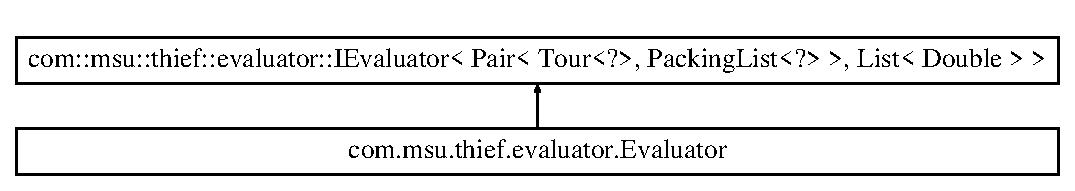
\includegraphics[height=2.000000cm]{classcom_1_1msu_1_1thief_1_1evaluator_1_1Evaluator}
\end{center}
\end{figure}
\subsection*{Public Member Functions}
\begin{DoxyCompactItemize}
\item 
\hypertarget{classcom_1_1msu_1_1thief_1_1evaluator_1_1Evaluator_a788b3eae58a8a6ac94080b1950418940}{{\bfseries Evaluator} (\hyperlink{classcom_1_1msu_1_1thief_1_1problems_1_1TravellingThiefProblem}{Travelling\-Thief\-Problem} problem, \hyperlink{classcom_1_1msu_1_1thief_1_1evaluator_1_1profit_1_1ProfitEvaluator}{Profit\-Evaluator} eval\-Profit, \hyperlink{classcom_1_1msu_1_1thief_1_1evaluator_1_1time_1_1TimeEvaluator}{Time\-Evaluator} eval\-Time)}\label{classcom_1_1msu_1_1thief_1_1evaluator_1_1Evaluator_a788b3eae58a8a6ac94080b1950418940}

\item 
\hypertarget{classcom_1_1msu_1_1thief_1_1evaluator_1_1Evaluator_aec1e3a841ab1a5a10ba95b41ae83ac19}{List$<$ Double $>$ {\bfseries evaluate} (Pair$<$ Tour$<$?$>$, Packing\-List$<$?$>$$>$ input)}\label{classcom_1_1msu_1_1thief_1_1evaluator_1_1Evaluator_aec1e3a841ab1a5a10ba95b41ae83ac19}

\end{DoxyCompactItemize}
\subsection*{Protected Attributes}
\begin{DoxyCompactItemize}
\item 
\hypertarget{classcom_1_1msu_1_1thief_1_1evaluator_1_1Evaluator_ac14bccab822220ede780c825a5fe3a78}{\hyperlink{classcom_1_1msu_1_1thief_1_1problems_1_1TravellingThiefProblem}{Travelling\-Thief\-Problem} {\bfseries problem} = null}\label{classcom_1_1msu_1_1thief_1_1evaluator_1_1Evaluator_ac14bccab822220ede780c825a5fe3a78}

\item 
\hypertarget{classcom_1_1msu_1_1thief_1_1evaluator_1_1Evaluator_a1a7984bc5332cfac89f627ff68ef64f0}{\hyperlink{classcom_1_1msu_1_1thief_1_1evaluator_1_1profit_1_1ProfitEvaluator}{Profit\-Evaluator} {\bfseries eval\-Profit} = null}\label{classcom_1_1msu_1_1thief_1_1evaluator_1_1Evaluator_a1a7984bc5332cfac89f627ff68ef64f0}

\item 
\hypertarget{classcom_1_1msu_1_1thief_1_1evaluator_1_1Evaluator_ad8291526450acab3521f300676caf060}{\hyperlink{classcom_1_1msu_1_1thief_1_1evaluator_1_1time_1_1TimeEvaluator}{Time\-Evaluator} {\bfseries eval\-Time} = null}\label{classcom_1_1msu_1_1thief_1_1evaluator_1_1Evaluator_ad8291526450acab3521f300676caf060}

\end{DoxyCompactItemize}


The documentation for this class was generated from the following file\-:\begin{DoxyCompactItemize}
\item 
src/main/java/com/msu/thief/evaluator/Evaluator.\-java\end{DoxyCompactItemize}

\hypertarget{classcom_1_1msu_1_1thief_1_1algorithms_1_1ExhaustiveKnapsack}{\section{com.\-msu.\-thief.\-algorithms.\-Exhaustive\-Knapsack Class Reference}
\label{classcom_1_1msu_1_1thief_1_1algorithms_1_1ExhaustiveKnapsack}\index{com.\-msu.\-thief.\-algorithms.\-Exhaustive\-Knapsack@{com.\-msu.\-thief.\-algorithms.\-Exhaustive\-Knapsack}}
}
Inheritance diagram for com.\-msu.\-thief.\-algorithms.\-Exhaustive\-Knapsack\-:\begin{figure}[H]
\begin{center}
\leavevmode
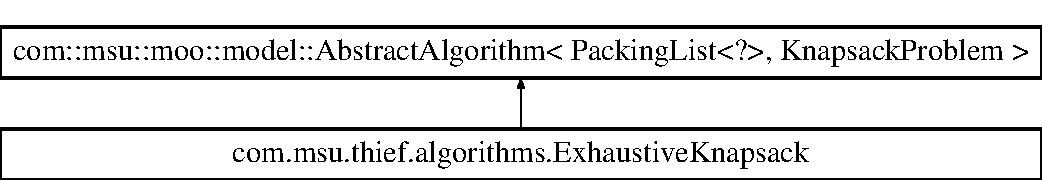
\includegraphics[height=2.000000cm]{classcom_1_1msu_1_1thief_1_1algorithms_1_1ExhaustiveKnapsack}
\end{center}
\end{figure}
\subsection*{Protected Member Functions}
\begin{DoxyCompactItemize}
\item 
\hypertarget{classcom_1_1msu_1_1thief_1_1algorithms_1_1ExhaustiveKnapsack_acf066c1e772d9a05b1530d9107fb4b02}{void {\bfseries next} ()}\label{classcom_1_1msu_1_1thief_1_1algorithms_1_1ExhaustiveKnapsack_acf066c1e772d9a05b1530d9107fb4b02}

\item 
\hypertarget{classcom_1_1msu_1_1thief_1_1algorithms_1_1ExhaustiveKnapsack_ae333b319b4e46506d8215e3be823de68}{Non\-Dominated\-Solution\-Set {\bfseries get\-Result} ()}\label{classcom_1_1msu_1_1thief_1_1algorithms_1_1ExhaustiveKnapsack_ae333b319b4e46506d8215e3be823de68}

\end{DoxyCompactItemize}
\subsection*{Protected Attributes}
\begin{DoxyCompactItemize}
\item 
\hypertarget{classcom_1_1msu_1_1thief_1_1algorithms_1_1ExhaustiveKnapsack_a0f39a710461d6fa8fdcc9523ad12d690}{Non\-Dominated\-Solution\-Set {\bfseries set}}\label{classcom_1_1msu_1_1thief_1_1algorithms_1_1ExhaustiveKnapsack_a0f39a710461d6fa8fdcc9523ad12d690}

\end{DoxyCompactItemize}


The documentation for this class was generated from the following file\-:\begin{DoxyCompactItemize}
\item 
src/main/java/com/msu/thief/algorithms/Exhaustive\-Knapsack.\-java\end{DoxyCompactItemize}

\hypertarget{classcom_1_1msu_1_1thief_1_1ExperimentExecutor}{\section{com.\-msu.\-thief.\-Experiment\-Executor Class Reference}
\label{classcom_1_1msu_1_1thief_1_1ExperimentExecutor}\index{com.\-msu.\-thief.\-Experiment\-Executor@{com.\-msu.\-thief.\-Experiment\-Executor}}
}
\subsection*{Static Public Member Functions}
\begin{DoxyCompactItemize}
\item 
\hypertarget{classcom_1_1msu_1_1thief_1_1ExperimentExecutor_ad642dd9f5e08bceed0e8f2d08bc11729}{static void {\bfseries main} (String\mbox{[}$\,$\mbox{]} args)}\label{classcom_1_1msu_1_1thief_1_1ExperimentExecutor_ad642dd9f5e08bceed0e8f2d08bc11729}

\end{DoxyCompactItemize}
\subsection*{Static Protected Attributes}
\begin{DoxyCompactItemize}
\item 
\hypertarget{classcom_1_1msu_1_1thief_1_1ExperimentExecutor_aca5fcadd393be1d2217c4ab115b3429d}{static final String \hyperlink{classcom_1_1msu_1_1thief_1_1ExperimentExecutor_aca5fcadd393be1d2217c4ab115b3429d}{E\-X\-P\-E\-R\-I\-M\-E\-N\-T} = \char`\"{}com.\-msu.\-thief.\-experiment.\-Greedy\-Map\-Experiment\char`\"{}}\label{classcom_1_1msu_1_1thief_1_1ExperimentExecutor_aca5fcadd393be1d2217c4ab115b3429d}

\begin{DoxyCompactList}\small\item\em experiment that should be executed \end{DoxyCompactList}\item 
\hypertarget{classcom_1_1msu_1_1thief_1_1ExperimentExecutor_ac1bc99ce39c691208254816b6b6b25f1}{static final int \hyperlink{classcom_1_1msu_1_1thief_1_1ExperimentExecutor_ac1bc99ce39c691208254816b6b6b25f1}{I\-T\-E\-R\-A\-T\-I\-O\-N\-S} = 1}\label{classcom_1_1msu_1_1thief_1_1ExperimentExecutor_ac1bc99ce39c691208254816b6b6b25f1}

\begin{DoxyCompactList}\small\item\em number of iterations per experiment \end{DoxyCompactList}\item 
\hypertarget{classcom_1_1msu_1_1thief_1_1ExperimentExecutor_aad994fb9a65c03a9bf55cb61a8d3a6c2}{static final long \hyperlink{classcom_1_1msu_1_1thief_1_1ExperimentExecutor_aad994fb9a65c03a9bf55cb61a8d3a6c2}{M\-A\-X\-\_\-\-E\-V\-A\-L\-U\-A\-T\-I\-O\-N\-S} = 100000}\label{classcom_1_1msu_1_1thief_1_1ExperimentExecutor_aad994fb9a65c03a9bf55cb61a8d3a6c2}

\begin{DoxyCompactList}\small\item\em max evaluations per run \end{DoxyCompactList}\item 
\hypertarget{classcom_1_1msu_1_1thief_1_1ExperimentExecutor_a48f961c14e062053b22b3857316bfde8}{static final long \hyperlink{classcom_1_1msu_1_1thief_1_1ExperimentExecutor_a48f961c14e062053b22b3857316bfde8}{S\-E\-E\-D} = 543453}\label{classcom_1_1msu_1_1thief_1_1ExperimentExecutor_a48f961c14e062053b22b3857316bfde8}

\begin{DoxyCompactList}\small\item\em random seed for experiment execution \end{DoxyCompactList}\end{DoxyCompactItemize}


The documentation for this class was generated from the following file\-:\begin{DoxyCompactItemize}
\item 
src/main/java/com/msu/thief/Experiment\-Executor.\-java\end{DoxyCompactItemize}

\hypertarget{classcom_1_1msu_1_1thief_1_1evaluator_1_1profit_1_1ExponentialProfitEvaluator}{\section{com.\-msu.\-thief.\-evaluator.\-profit.\-Exponential\-Profit\-Evaluator Class Reference}
\label{classcom_1_1msu_1_1thief_1_1evaluator_1_1profit_1_1ExponentialProfitEvaluator}\index{com.\-msu.\-thief.\-evaluator.\-profit.\-Exponential\-Profit\-Evaluator@{com.\-msu.\-thief.\-evaluator.\-profit.\-Exponential\-Profit\-Evaluator}}
}
Inheritance diagram for com.\-msu.\-thief.\-evaluator.\-profit.\-Exponential\-Profit\-Evaluator\-:\begin{figure}[H]
\begin{center}
\leavevmode
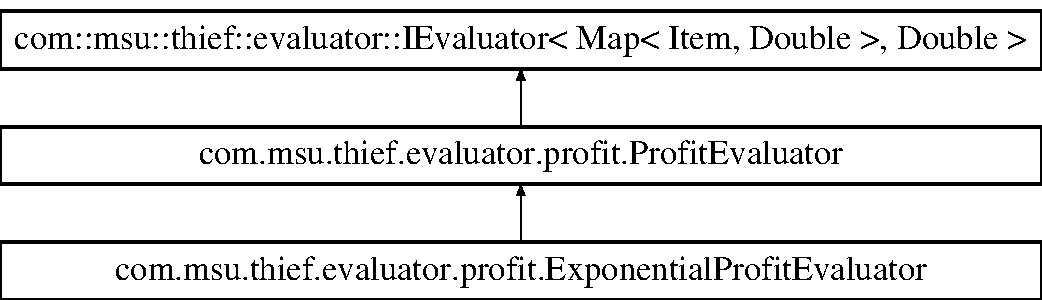
\includegraphics[height=3.000000cm]{classcom_1_1msu_1_1thief_1_1evaluator_1_1profit_1_1ExponentialProfitEvaluator}
\end{center}
\end{figure}
\subsection*{Public Member Functions}
\begin{DoxyCompactItemize}
\item 
\hypertarget{classcom_1_1msu_1_1thief_1_1evaluator_1_1profit_1_1ExponentialProfitEvaluator_a78cbc6e5d473b049534795b7fe154d31}{{\bfseries Exponential\-Profit\-Evaluator} (double \hyperlink{classcom_1_1msu_1_1thief_1_1evaluator_1_1profit_1_1ExponentialProfitEvaluator_a0bee5d7f079a9676692e3faa5f9d2da9}{dropping\-Rate}, double \hyperlink{classcom_1_1msu_1_1thief_1_1evaluator_1_1profit_1_1ExponentialProfitEvaluator_a75237d11c10af36c7f466e462d25d894}{dropping\-Constant})}\label{classcom_1_1msu_1_1thief_1_1evaluator_1_1profit_1_1ExponentialProfitEvaluator_a78cbc6e5d473b049534795b7fe154d31}

\item 
\hypertarget{classcom_1_1msu_1_1thief_1_1evaluator_1_1profit_1_1ExponentialProfitEvaluator_a5c38554b21eebe25127a9c79624db60b}{Double {\bfseries evaluate} (Map$<$ \hyperlink{classcom_1_1msu_1_1thief_1_1model_1_1Item}{Item}, Double $>$ m\-Items)}\label{classcom_1_1msu_1_1thief_1_1evaluator_1_1profit_1_1ExponentialProfitEvaluator_a5c38554b21eebe25127a9c79624db60b}

\end{DoxyCompactItemize}
\subsection*{Protected Attributes}
\begin{DoxyCompactItemize}
\item 
\hypertarget{classcom_1_1msu_1_1thief_1_1evaluator_1_1profit_1_1ExponentialProfitEvaluator_a0bee5d7f079a9676692e3faa5f9d2da9}{double \hyperlink{classcom_1_1msu_1_1thief_1_1evaluator_1_1profit_1_1ExponentialProfitEvaluator_a0bee5d7f079a9676692e3faa5f9d2da9}{dropping\-Rate} = 0.\-9}\label{classcom_1_1msu_1_1thief_1_1evaluator_1_1profit_1_1ExponentialProfitEvaluator_a0bee5d7f079a9676692e3faa5f9d2da9}

\begin{DoxyCompactList}\small\item\em dropping rate over time \end{DoxyCompactList}\item 
\hypertarget{classcom_1_1msu_1_1thief_1_1evaluator_1_1profit_1_1ExponentialProfitEvaluator_a75237d11c10af36c7f466e462d25d894}{double \hyperlink{classcom_1_1msu_1_1thief_1_1evaluator_1_1profit_1_1ExponentialProfitEvaluator_a75237d11c10af36c7f466e462d25d894}{dropping\-Constant} = 10}\label{classcom_1_1msu_1_1thief_1_1evaluator_1_1profit_1_1ExponentialProfitEvaluator_a75237d11c10af36c7f466e462d25d894}

\begin{DoxyCompactList}\small\item\em dropping constant for tuning the large distances \end{DoxyCompactList}\end{DoxyCompactItemize}


\subsection{Detailed Description}
The Exponential\-Profit\-Calculator uses the same function for all items. 

The documentation for this class was generated from the following file\-:\begin{DoxyCompactItemize}
\item 
src/main/java/com/msu/thief/evaluator/profit/Exponential\-Profit\-Evaluator.\-java\end{DoxyCompactItemize}

\hypertarget{classcom_1_1msu_1_1thief_1_1util_1_1Factory}{\section{com.\-msu.\-thief.\-util.\-Factory Class Reference}
\label{classcom_1_1msu_1_1thief_1_1util_1_1Factory}\index{com.\-msu.\-thief.\-util.\-Factory@{com.\-msu.\-thief.\-util.\-Factory}}
}
\subsection*{Static Public Member Functions}
\begin{DoxyCompactItemize}
\item 
\hypertarget{classcom_1_1msu_1_1thief_1_1util_1_1Factory_a6f91155d61cb2c8290d089162434de62}{static Object {\bfseries create} (String full\-Type)}\label{classcom_1_1msu_1_1thief_1_1util_1_1Factory_a6f91155d61cb2c8290d089162434de62}

\item 
\hypertarget{classcom_1_1msu_1_1thief_1_1util_1_1Factory_a5ee4815cc5f9ad36e6d3dc4e920d63d0}{static$<$ T $>$ T {\bfseries create} (Class$<$ T $>$ c, String full\-Type)}\label{classcom_1_1msu_1_1thief_1_1util_1_1Factory_a5ee4815cc5f9ad36e6d3dc4e920d63d0}

\end{DoxyCompactItemize}


The documentation for this class was generated from the following file\-:\begin{DoxyCompactItemize}
\item 
src/main/java/com/msu/thief/util/Factory.\-java\end{DoxyCompactItemize}

\hypertarget{classcom_1_1msu_1_1thief_1_1experiment_1_1GreedyMapExperiment}{\section{com.\-msu.\-thief.\-experiment.\-Greedy\-Map\-Experiment Class Reference}
\label{classcom_1_1msu_1_1thief_1_1experiment_1_1GreedyMapExperiment}\index{com.\-msu.\-thief.\-experiment.\-Greedy\-Map\-Experiment@{com.\-msu.\-thief.\-experiment.\-Greedy\-Map\-Experiment}}
}
Inheritance diagram for com.\-msu.\-thief.\-experiment.\-Greedy\-Map\-Experiment\-:\begin{figure}[H]
\begin{center}
\leavevmode
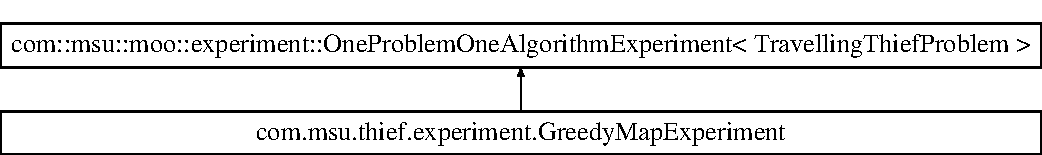
\includegraphics[height=2.000000cm]{classcom_1_1msu_1_1thief_1_1experiment_1_1GreedyMapExperiment}
\end{center}
\end{figure}
\subsection*{Public Member Functions}
\begin{DoxyCompactItemize}
\item 
\hypertarget{classcom_1_1msu_1_1thief_1_1experiment_1_1GreedyMapExperiment_acdc02b952bd9f3358cb2b336b7ec5b30}{void {\bfseries report} ()}\label{classcom_1_1msu_1_1thief_1_1experiment_1_1GreedyMapExperiment_acdc02b952bd9f3358cb2b336b7ec5b30}

\end{DoxyCompactItemize}
\subsection*{Protected Member Functions}
\begin{DoxyCompactItemize}
\item 
\hypertarget{classcom_1_1msu_1_1thief_1_1experiment_1_1GreedyMapExperiment_aa19f8414d42c297c2c26bab228ecee41}{I\-Algorithm\\*
$<$ \hyperlink{classcom_1_1msu_1_1thief_1_1problems_1_1TravellingThiefProblem}{Travelling\-Thief\-Problem} $>$ {\bfseries get\-Algorithm} ()}\label{classcom_1_1msu_1_1thief_1_1experiment_1_1GreedyMapExperiment_aa19f8414d42c297c2c26bab228ecee41}

\item 
\hypertarget{classcom_1_1msu_1_1thief_1_1experiment_1_1GreedyMapExperiment_a1b4ddd16cc4e6af8013a79f998f611b2}{\hyperlink{classcom_1_1msu_1_1thief_1_1problems_1_1TravellingThiefProblem}{Travelling\-Thief\-Problem} {\bfseries get\-Problem} ()}\label{classcom_1_1msu_1_1thief_1_1experiment_1_1GreedyMapExperiment_a1b4ddd16cc4e6af8013a79f998f611b2}

\item 
\hypertarget{classcom_1_1msu_1_1thief_1_1experiment_1_1GreedyMapExperiment_a2dbe890d03bc7855c17fa53f2f8dabe8}{Non\-Dominated\-Solution\-Set {\bfseries get\-True\-Front} ()}\label{classcom_1_1msu_1_1thief_1_1experiment_1_1GreedyMapExperiment_a2dbe890d03bc7855c17fa53f2f8dabe8}

\end{DoxyCompactItemize}
\subsection*{Protected Attributes}
\begin{DoxyCompactItemize}
\item 
\hypertarget{classcom_1_1msu_1_1thief_1_1experiment_1_1GreedyMapExperiment_ab136006a9abf32be8188424852a0ade1}{final int {\bfseries N\-U\-M\-\_\-\-O\-F\-\_\-\-C\-I\-T\-I\-E\-S} = 50}\label{classcom_1_1msu_1_1thief_1_1experiment_1_1GreedyMapExperiment_ab136006a9abf32be8188424852a0ade1}

\end{DoxyCompactItemize}


The documentation for this class was generated from the following file\-:\begin{DoxyCompactItemize}
\item 
src/main/java/com/msu/thief/experiment/Greedy\-Map\-Experiment.\-java\end{DoxyCompactItemize}

\hypertarget{interfacecom_1_1msu_1_1thief_1_1problems_1_1ICityProblem}{\section{com.\-msu.\-thief.\-problems.\-I\-City\-Problem Interface Reference}
\label{interfacecom_1_1msu_1_1thief_1_1problems_1_1ICityProblem}\index{com.\-msu.\-thief.\-problems.\-I\-City\-Problem@{com.\-msu.\-thief.\-problems.\-I\-City\-Problem}}
}
Inheritance diagram for com.\-msu.\-thief.\-problems.\-I\-City\-Problem\-:\begin{figure}[H]
\begin{center}
\leavevmode
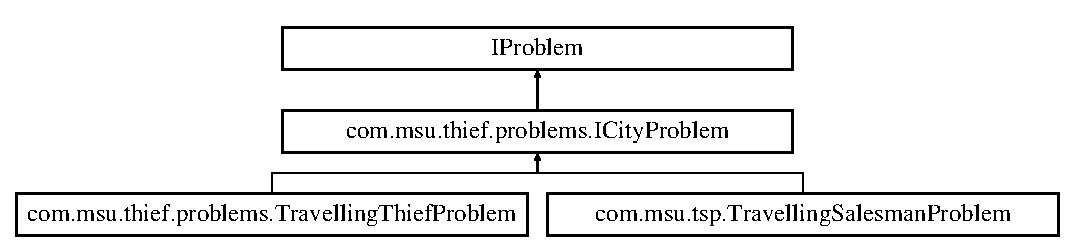
\includegraphics[height=2.937063cm]{interfacecom_1_1msu_1_1thief_1_1problems_1_1ICityProblem}
\end{center}
\end{figure}
\subsection*{Public Member Functions}
\begin{DoxyCompactItemize}
\item 
\hypertarget{interfacecom_1_1msu_1_1thief_1_1problems_1_1ICityProblem_a1092247b6bed5faf1c95d2169f8152c2}{int {\bfseries num\-Of\-Cities} ()}\label{interfacecom_1_1msu_1_1thief_1_1problems_1_1ICityProblem_a1092247b6bed5faf1c95d2169f8152c2}

\end{DoxyCompactItemize}


The documentation for this interface was generated from the following file\-:\begin{DoxyCompactItemize}
\item 
src/main/java/com/msu/thief/problems/I\-City\-Problem.\-java\end{DoxyCompactItemize}

\hypertarget{interfacecom_1_1msu_1_1thief_1_1evaluator_1_1IEvaluator_3_01I_00_01O_01_4}{\section{com.\-msu.\-thief.\-evaluator.\-I\-Evaluator$<$ I, O $>$ Interface Reference}
\label{interfacecom_1_1msu_1_1thief_1_1evaluator_1_1IEvaluator_3_01I_00_01O_01_4}\index{com.\-msu.\-thief.\-evaluator.\-I\-Evaluator$<$ I, O $>$@{com.\-msu.\-thief.\-evaluator.\-I\-Evaluator$<$ I, O $>$}}
}
\subsection*{Public Member Functions}
\begin{DoxyCompactItemize}
\item 
\hypertarget{interfacecom_1_1msu_1_1thief_1_1evaluator_1_1IEvaluator_3_01I_00_01O_01_4_a68d80ccfa17903fc1f1d3391084e7a35}{O {\bfseries evaluate} (I input)}\label{interfacecom_1_1msu_1_1thief_1_1evaluator_1_1IEvaluator_3_01I_00_01O_01_4_a68d80ccfa17903fc1f1d3391084e7a35}

\end{DoxyCompactItemize}


\subsection{Detailed Description}
Interface for evaluating any input to Double 
\begin{DoxyParams}{Parameters}
{\em $<$\-T$>$} & input of the evaluator \\
\hline
\end{DoxyParams}


The documentation for this interface was generated from the following file\-:\begin{DoxyCompactItemize}
\item 
src/main/java/com/msu/thief/evaluator/I\-Evaluator.\-java\end{DoxyCompactItemize}

\hypertarget{classcom_1_1msu_1_1thief_1_1evaluator_1_1profit_1_1IndividualProfitEvaluator}{\section{com.\-msu.\-thief.\-evaluator.\-profit.\-Individual\-Profit\-Evaluator Class Reference}
\label{classcom_1_1msu_1_1thief_1_1evaluator_1_1profit_1_1IndividualProfitEvaluator}\index{com.\-msu.\-thief.\-evaluator.\-profit.\-Individual\-Profit\-Evaluator@{com.\-msu.\-thief.\-evaluator.\-profit.\-Individual\-Profit\-Evaluator}}
}
Inheritance diagram for com.\-msu.\-thief.\-evaluator.\-profit.\-Individual\-Profit\-Evaluator\-:\begin{figure}[H]
\begin{center}
\leavevmode
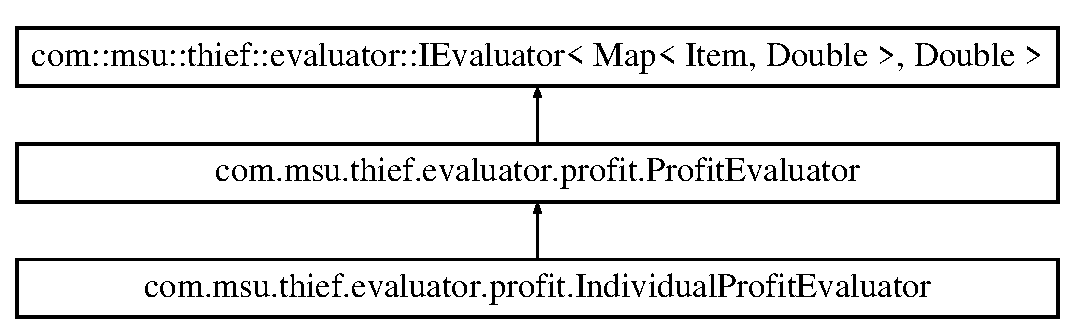
\includegraphics[height=3.000000cm]{classcom_1_1msu_1_1thief_1_1evaluator_1_1profit_1_1IndividualProfitEvaluator}
\end{center}
\end{figure}
\subsection*{Public Member Functions}
\begin{DoxyCompactItemize}
\item 
\hypertarget{classcom_1_1msu_1_1thief_1_1evaluator_1_1profit_1_1IndividualProfitEvaluator_add7fe39c2f4e010d8f0dbe204b5aaf57}{Double {\bfseries evaluate} (Map$<$ \hyperlink{classcom_1_1msu_1_1thief_1_1model_1_1Item}{Item}, Double $>$ m\-Items)}\label{classcom_1_1msu_1_1thief_1_1evaluator_1_1profit_1_1IndividualProfitEvaluator_add7fe39c2f4e010d8f0dbe204b5aaf57}

\end{DoxyCompactItemize}


\subsection{Detailed Description}
The Individual\-Profit\-Calculator calculates the profit by using a dropping rate for each item! 

The documentation for this class was generated from the following file\-:\begin{DoxyCompactItemize}
\item 
src/main/java/com/msu/thief/evaluator/profit/Individual\-Profit\-Evaluator.\-java\end{DoxyCompactItemize}

\hypertarget{interfacecom_1_1msu_1_1thief_1_1model_1_1packing_1_1IPackingPlanFactory}{\section{com.\-msu.\-thief.\-model.\-packing.\-I\-Packing\-Plan\-Factory Interface Reference}
\label{interfacecom_1_1msu_1_1thief_1_1model_1_1packing_1_1IPackingPlanFactory}\index{com.\-msu.\-thief.\-model.\-packing.\-I\-Packing\-Plan\-Factory@{com.\-msu.\-thief.\-model.\-packing.\-I\-Packing\-Plan\-Factory}}
}
Inheritance diagram for com.\-msu.\-thief.\-model.\-packing.\-I\-Packing\-Plan\-Factory\-:\begin{figure}[H]
\begin{center}
\leavevmode
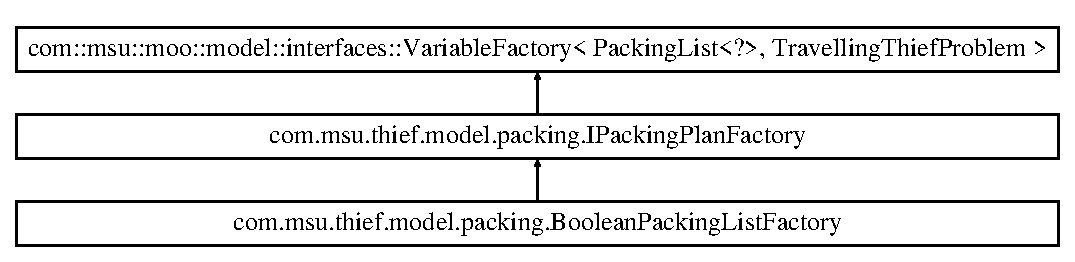
\includegraphics[height=3.000000cm]{interfacecom_1_1msu_1_1thief_1_1model_1_1packing_1_1IPackingPlanFactory}
\end{center}
\end{figure}
\subsection*{Public Member Functions}
\begin{DoxyCompactItemize}
\item 
\hypertarget{interfacecom_1_1msu_1_1thief_1_1model_1_1packing_1_1IPackingPlanFactory_af7feddd76ad5f7ab49b365720fad712c}{Packing\-List$<$?$>$ {\bfseries create} (\hyperlink{classcom_1_1msu_1_1thief_1_1problems_1_1TravellingThiefProblem}{Travelling\-Thief\-Problem} p)}\label{interfacecom_1_1msu_1_1thief_1_1model_1_1packing_1_1IPackingPlanFactory_af7feddd76ad5f7ab49b365720fad712c}

\end{DoxyCompactItemize}


The documentation for this interface was generated from the following file\-:\begin{DoxyCompactItemize}
\item 
src/main/java/com/msu/thief/model/packing/I\-Packing\-Plan\-Factory.\-java\end{DoxyCompactItemize}

\hypertarget{interfacecom_1_1msu_1_1thief_1_1problems_1_1IPackingProblem}{\section{com.\-msu.\-thief.\-problems.\-I\-Packing\-Problem Interface Reference}
\label{interfacecom_1_1msu_1_1thief_1_1problems_1_1IPackingProblem}\index{com.\-msu.\-thief.\-problems.\-I\-Packing\-Problem@{com.\-msu.\-thief.\-problems.\-I\-Packing\-Problem}}
}
Inheritance diagram for com.\-msu.\-thief.\-problems.\-I\-Packing\-Problem\-:\begin{figure}[H]
\begin{center}
\leavevmode
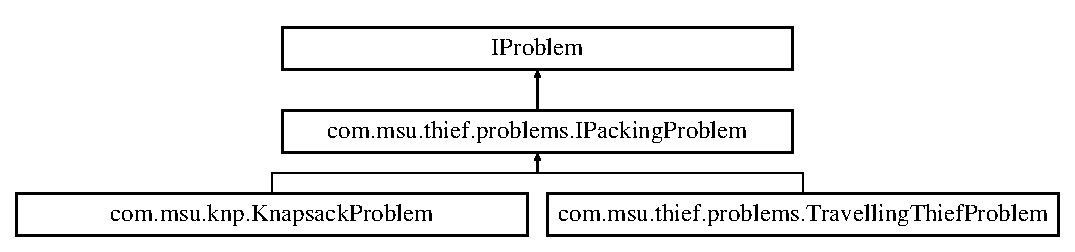
\includegraphics[height=2.937063cm]{interfacecom_1_1msu_1_1thief_1_1problems_1_1IPackingProblem}
\end{center}
\end{figure}
\subsection*{Public Member Functions}
\begin{DoxyCompactItemize}
\item 
\hypertarget{interfacecom_1_1msu_1_1thief_1_1problems_1_1IPackingProblem_ab5d3f9128f77797d660f9372e7459297}{int {\bfseries num\-Of\-Items} ()}\label{interfacecom_1_1msu_1_1thief_1_1problems_1_1IPackingProblem_ab5d3f9128f77797d660f9372e7459297}

\end{DoxyCompactItemize}


The documentation for this interface was generated from the following file\-:\begin{DoxyCompactItemize}
\item 
src/main/java/com/msu/thief/problems/I\-Packing\-Problem.\-java\end{DoxyCompactItemize}

\hypertarget{classcom_1_1msu_1_1thief_1_1model_1_1Item}{\section{com.\-msu.\-thief.\-model.\-Item Class Reference}
\label{classcom_1_1msu_1_1thief_1_1model_1_1Item}\index{com.\-msu.\-thief.\-model.\-Item@{com.\-msu.\-thief.\-model.\-Item}}
}
\subsection*{Public Member Functions}
\begin{DoxyCompactItemize}
\item 
\hyperlink{classcom_1_1msu_1_1thief_1_1model_1_1Item_ac7b6aa0e8258962aceb32f64fb098548}{Item} (double \hyperlink{classcom_1_1msu_1_1thief_1_1model_1_1Item_a540f0be6af9387af62bf43bf2930a4da}{profit}, double \hyperlink{classcom_1_1msu_1_1thief_1_1model_1_1Item_a2a6b0a03bfff2ac46c09d972a52a063e}{weight})
\item 
\hyperlink{classcom_1_1msu_1_1thief_1_1model_1_1Item_a31e0ccadcc133e909e37347a3316c860}{Item} (double \hyperlink{classcom_1_1msu_1_1thief_1_1model_1_1Item_a540f0be6af9387af62bf43bf2930a4da}{profit}, double \hyperlink{classcom_1_1msu_1_1thief_1_1model_1_1Item_a2a6b0a03bfff2ac46c09d972a52a063e}{weight}, double \hyperlink{classcom_1_1msu_1_1thief_1_1model_1_1Item_acdbd5c173fae33c3f321caeed8a373df}{dropping})
\item 
\hypertarget{classcom_1_1msu_1_1thief_1_1model_1_1Item_a3ed58b8b54b8819a026651a4646acec5}{double {\bfseries get\-Weight} ()}\label{classcom_1_1msu_1_1thief_1_1model_1_1Item_a3ed58b8b54b8819a026651a4646acec5}

\item 
\hypertarget{classcom_1_1msu_1_1thief_1_1model_1_1Item_a884e3820b56b01474d5b49c86b45e045}{double {\bfseries get\-Profit} ()}\label{classcom_1_1msu_1_1thief_1_1model_1_1Item_a884e3820b56b01474d5b49c86b45e045}

\item 
\hypertarget{classcom_1_1msu_1_1thief_1_1model_1_1Item_a03d6c8ea96d614165efc37f0227d5c14}{double {\bfseries get\-Dropping} ()}\label{classcom_1_1msu_1_1thief_1_1model_1_1Item_a03d6c8ea96d614165efc37f0227d5c14}

\item 
\hypertarget{classcom_1_1msu_1_1thief_1_1model_1_1Item_a46c474b03929cae07e94eb5bfc95c8e1}{String {\bfseries to\-String} ()}\label{classcom_1_1msu_1_1thief_1_1model_1_1Item_a46c474b03929cae07e94eb5bfc95c8e1}

\end{DoxyCompactItemize}
\subsection*{Protected Attributes}
\begin{DoxyCompactItemize}
\item 
\hypertarget{classcom_1_1msu_1_1thief_1_1model_1_1Item_a2a6b0a03bfff2ac46c09d972a52a063e}{double \hyperlink{classcom_1_1msu_1_1thief_1_1model_1_1Item_a2a6b0a03bfff2ac46c09d972a52a063e}{weight}}\label{classcom_1_1msu_1_1thief_1_1model_1_1Item_a2a6b0a03bfff2ac46c09d972a52a063e}

\begin{DoxyCompactList}\small\item\em weight of the item \end{DoxyCompactList}\item 
\hypertarget{classcom_1_1msu_1_1thief_1_1model_1_1Item_a540f0be6af9387af62bf43bf2930a4da}{double \hyperlink{classcom_1_1msu_1_1thief_1_1model_1_1Item_a540f0be6af9387af62bf43bf2930a4da}{profit}}\label{classcom_1_1msu_1_1thief_1_1model_1_1Item_a540f0be6af9387af62bf43bf2930a4da}

\begin{DoxyCompactList}\small\item\em profit of the item \end{DoxyCompactList}\item 
\hypertarget{classcom_1_1msu_1_1thief_1_1model_1_1Item_acdbd5c173fae33c3f321caeed8a373df}{double \hyperlink{classcom_1_1msu_1_1thief_1_1model_1_1Item_acdbd5c173fae33c3f321caeed8a373df}{dropping}}\label{classcom_1_1msu_1_1thief_1_1model_1_1Item_acdbd5c173fae33c3f321caeed8a373df}

\begin{DoxyCompactList}\small\item\em dropping of the item over time \end{DoxyCompactList}\end{DoxyCompactItemize}


\subsection{Detailed Description}
This class represents an item that could be picked by the salesman or selected for the knapsack. The attributes are the weight and profit. 

\subsection{Constructor \& Destructor Documentation}
\hypertarget{classcom_1_1msu_1_1thief_1_1model_1_1Item_ac7b6aa0e8258962aceb32f64fb098548}{\index{com\-::msu\-::thief\-::model\-::\-Item@{com\-::msu\-::thief\-::model\-::\-Item}!Item@{Item}}
\index{Item@{Item}!com::msu::thief::model::Item@{com\-::msu\-::thief\-::model\-::\-Item}}
\subsubsection[{Item}]{\setlength{\rightskip}{0pt plus 5cm}com.\-msu.\-thief.\-model.\-Item.\-Item (
\begin{DoxyParamCaption}
\item[{double}]{profit, }
\item[{double}]{weight}
\end{DoxyParamCaption}
)\hspace{0.3cm}{\ttfamily [inline]}}}\label{classcom_1_1msu_1_1thief_1_1model_1_1Item_ac7b6aa0e8258962aceb32f64fb098548}
Create an item with predefined values. \hypertarget{classcom_1_1msu_1_1thief_1_1model_1_1Item_a31e0ccadcc133e909e37347a3316c860}{\index{com\-::msu\-::thief\-::model\-::\-Item@{com\-::msu\-::thief\-::model\-::\-Item}!Item@{Item}}
\index{Item@{Item}!com::msu::thief::model::Item@{com\-::msu\-::thief\-::model\-::\-Item}}
\subsubsection[{Item}]{\setlength{\rightskip}{0pt plus 5cm}com.\-msu.\-thief.\-model.\-Item.\-Item (
\begin{DoxyParamCaption}
\item[{double}]{profit, }
\item[{double}]{weight, }
\item[{double}]{dropping}
\end{DoxyParamCaption}
)\hspace{0.3cm}{\ttfamily [inline]}}}\label{classcom_1_1msu_1_1thief_1_1model_1_1Item_a31e0ccadcc133e909e37347a3316c860}
Create an item with profit,weight and dropping. 

The documentation for this class was generated from the following file\-:\begin{DoxyCompactItemize}
\item 
src/main/java/com/msu/thief/model/Item.\-java\end{DoxyCompactItemize}

\hypertarget{classcom_1_1msu_1_1thief_1_1model_1_1ItemCollection_3_01T_01extends_01Item_01_4}{\section{com.\-msu.\-thief.\-model.\-Item\-Collection$<$ T extends Item $>$ Class Reference}
\label{classcom_1_1msu_1_1thief_1_1model_1_1ItemCollection_3_01T_01extends_01Item_01_4}\index{com.\-msu.\-thief.\-model.\-Item\-Collection$<$ T extends Item $>$@{com.\-msu.\-thief.\-model.\-Item\-Collection$<$ T extends Item $>$}}
}
Inheritance diagram for com.\-msu.\-thief.\-model.\-Item\-Collection$<$ T extends Item $>$\-:\begin{figure}[H]
\begin{center}
\leavevmode
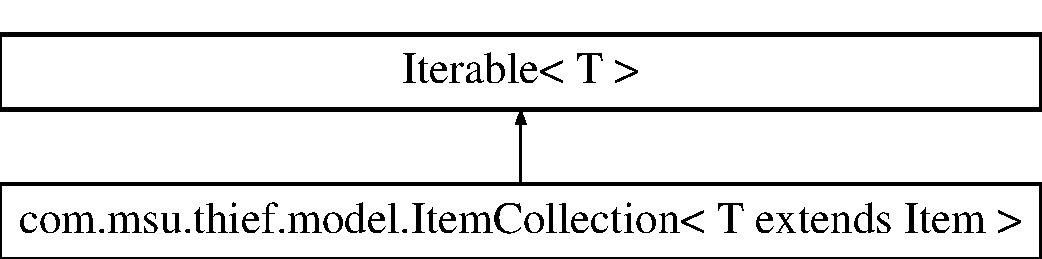
\includegraphics[height=2.000000cm]{classcom_1_1msu_1_1thief_1_1model_1_1ItemCollection_3_01T_01extends_01Item_01_4}
\end{center}
\end{figure}
\subsection*{Public Member Functions}
\begin{DoxyCompactItemize}
\item 
\hypertarget{classcom_1_1msu_1_1thief_1_1model_1_1ItemCollection_3_01T_01extends_01Item_01_4_a81bcb2492a8fc8324338fc9c93d243b4}{Iterator$<$ T $>$ {\bfseries iterator} ()}\label{classcom_1_1msu_1_1thief_1_1model_1_1ItemCollection_3_01T_01extends_01Item_01_4_a81bcb2492a8fc8324338fc9c93d243b4}

\item 
void \hyperlink{classcom_1_1msu_1_1thief_1_1model_1_1ItemCollection_3_01T_01extends_01Item_01_4_a11bea9852ef956861f92527831083aac}{add} (int city, T item)
\item 
List$<$ T $>$ \hyperlink{classcom_1_1msu_1_1thief_1_1model_1_1ItemCollection_3_01T_01extends_01Item_01_4_a8ba2465ea966528d155028525f417702}{get\-Items} ()
\item 
boolean \hyperlink{classcom_1_1msu_1_1thief_1_1model_1_1ItemCollection_3_01T_01extends_01Item_01_4_a82d96f8e83739b321cc185119481f770}{is\-Item\-At\-City} (int city, T item)
\item 
List$<$ T $>$ \hyperlink{classcom_1_1msu_1_1thief_1_1model_1_1ItemCollection_3_01T_01extends_01Item_01_4_a3d2560312732695c625bc083bc440761}{get\-Items\-From\-City} (int city)
\item 
Set$<$ Integer $>$ \hyperlink{classcom_1_1msu_1_1thief_1_1model_1_1ItemCollection_3_01T_01extends_01Item_01_4_a87765ea1b66b6a31d89679c9ca768413}{get\-Items\-From\-City\-By\-Index} (int city)
\item 
\hypertarget{classcom_1_1msu_1_1thief_1_1model_1_1ItemCollection_3_01T_01extends_01Item_01_4_a61467644747e6a702b72abad14bb12ac}{int {\bfseries size} ()}\label{classcom_1_1msu_1_1thief_1_1model_1_1ItemCollection_3_01T_01extends_01Item_01_4_a61467644747e6a702b72abad14bb12ac}

\item 
\hypertarget{classcom_1_1msu_1_1thief_1_1model_1_1ItemCollection_3_01T_01extends_01Item_01_4_aee431beb012ef3de53ade3cdf59a4131}{\hyperlink{classcom_1_1msu_1_1thief_1_1model_1_1Item}{Item} {\bfseries get} (int i)}\label{classcom_1_1msu_1_1thief_1_1model_1_1ItemCollection_3_01T_01extends_01Item_01_4_aee431beb012ef3de53ade3cdf59a4131}

\end{DoxyCompactItemize}
\subsection*{Protected Attributes}
\begin{DoxyCompactItemize}
\item 
\hypertarget{classcom_1_1msu_1_1thief_1_1model_1_1ItemCollection_3_01T_01extends_01Item_01_4_a678804cba392f7ba8be19313f8b48c15}{Array\-List$<$ T $>$ {\bfseries items}}\label{classcom_1_1msu_1_1thief_1_1model_1_1ItemCollection_3_01T_01extends_01Item_01_4_a678804cba392f7ba8be19313f8b48c15}

\item 
\hypertarget{classcom_1_1msu_1_1thief_1_1model_1_1ItemCollection_3_01T_01extends_01Item_01_4_abdafcfaf4a7dbae104fd5b4e16f20b69}{Hash\-Multimap$<$ Integer, Integer $>$ {\bfseries map\-From\-City\-To\-Item}}\label{classcom_1_1msu_1_1thief_1_1model_1_1ItemCollection_3_01T_01extends_01Item_01_4_abdafcfaf4a7dbae104fd5b4e16f20b69}

\item 
\hypertarget{classcom_1_1msu_1_1thief_1_1model_1_1ItemCollection_3_01T_01extends_01Item_01_4_a7c4263b1bf9c6a5b7404db3247abe598}{Hash\-Map$<$ Integer, Integer $>$ {\bfseries map\-From\-Item\-To\-City}}\label{classcom_1_1msu_1_1thief_1_1model_1_1ItemCollection_3_01T_01extends_01Item_01_4_a7c4263b1bf9c6a5b7404db3247abe598}

\end{DoxyCompactItemize}


\subsection{Detailed Description}
This class represents a Item\-Collection that maps each item to a city. Several utility structures are used to provide fast access. 
\begin{DoxyParams}{Parameters}
{\em $<$\-T$>$} & \hyperlink{classcom_1_1msu_1_1thief_1_1model_1_1Item}{Item} class or inherited one! \\
\hline
\end{DoxyParams}


\subsection{Member Function Documentation}
\hypertarget{classcom_1_1msu_1_1thief_1_1model_1_1ItemCollection_3_01T_01extends_01Item_01_4_a11bea9852ef956861f92527831083aac}{\index{com\-::msu\-::thief\-::model\-::\-Item\-Collection$<$ T extends Item $>$@{com\-::msu\-::thief\-::model\-::\-Item\-Collection$<$ T extends Item $>$}!add@{add}}
\index{add@{add}!com::msu::thief::model::ItemCollection< T extends Item >@{com\-::msu\-::thief\-::model\-::\-Item\-Collection$<$ T extends Item $>$}}
\subsubsection[{add}]{\setlength{\rightskip}{0pt plus 5cm}void com.\-msu.\-thief.\-model.\-Item\-Collection$<$ T extends {\bf Item} $>$.add (
\begin{DoxyParamCaption}
\item[{int}]{city, }
\item[{T}]{item}
\end{DoxyParamCaption}
)\hspace{0.3cm}{\ttfamily [inline]}}}\label{classcom_1_1msu_1_1thief_1_1model_1_1ItemCollection_3_01T_01extends_01Item_01_4_a11bea9852ef956861f92527831083aac}
Add an item to a city. \hypertarget{classcom_1_1msu_1_1thief_1_1model_1_1ItemCollection_3_01T_01extends_01Item_01_4_a8ba2465ea966528d155028525f417702}{\index{com\-::msu\-::thief\-::model\-::\-Item\-Collection$<$ T extends Item $>$@{com\-::msu\-::thief\-::model\-::\-Item\-Collection$<$ T extends Item $>$}!get\-Items@{get\-Items}}
\index{get\-Items@{get\-Items}!com::msu::thief::model::ItemCollection< T extends Item >@{com\-::msu\-::thief\-::model\-::\-Item\-Collection$<$ T extends Item $>$}}
\subsubsection[{get\-Items}]{\setlength{\rightskip}{0pt plus 5cm}List$<$T$>$ com.\-msu.\-thief.\-model.\-Item\-Collection$<$ T extends {\bf Item} $>$.get\-Items (
\begin{DoxyParamCaption}
{}
\end{DoxyParamCaption}
)\hspace{0.3cm}{\ttfamily [inline]}}}\label{classcom_1_1msu_1_1thief_1_1model_1_1ItemCollection_3_01T_01extends_01Item_01_4_a8ba2465ea966528d155028525f417702}
\begin{DoxyReturn}{Returns}
items as a vector 
\end{DoxyReturn}
\hypertarget{classcom_1_1msu_1_1thief_1_1model_1_1ItemCollection_3_01T_01extends_01Item_01_4_a3d2560312732695c625bc083bc440761}{\index{com\-::msu\-::thief\-::model\-::\-Item\-Collection$<$ T extends Item $>$@{com\-::msu\-::thief\-::model\-::\-Item\-Collection$<$ T extends Item $>$}!get\-Items\-From\-City@{get\-Items\-From\-City}}
\index{get\-Items\-From\-City@{get\-Items\-From\-City}!com::msu::thief::model::ItemCollection< T extends Item >@{com\-::msu\-::thief\-::model\-::\-Item\-Collection$<$ T extends Item $>$}}
\subsubsection[{get\-Items\-From\-City}]{\setlength{\rightskip}{0pt plus 5cm}List$<$T$>$ com.\-msu.\-thief.\-model.\-Item\-Collection$<$ T extends {\bf Item} $>$.get\-Items\-From\-City (
\begin{DoxyParamCaption}
\item[{int}]{city}
\end{DoxyParamCaption}
)\hspace{0.3cm}{\ttfamily [inline]}}}\label{classcom_1_1msu_1_1thief_1_1model_1_1ItemCollection_3_01T_01extends_01Item_01_4_a3d2560312732695c625bc083bc440761}
\begin{DoxyReturn}{Returns}
all items that are at the specific city. 
\end{DoxyReturn}
\hypertarget{classcom_1_1msu_1_1thief_1_1model_1_1ItemCollection_3_01T_01extends_01Item_01_4_a87765ea1b66b6a31d89679c9ca768413}{\index{com\-::msu\-::thief\-::model\-::\-Item\-Collection$<$ T extends Item $>$@{com\-::msu\-::thief\-::model\-::\-Item\-Collection$<$ T extends Item $>$}!get\-Items\-From\-City\-By\-Index@{get\-Items\-From\-City\-By\-Index}}
\index{get\-Items\-From\-City\-By\-Index@{get\-Items\-From\-City\-By\-Index}!com::msu::thief::model::ItemCollection< T extends Item >@{com\-::msu\-::thief\-::model\-::\-Item\-Collection$<$ T extends Item $>$}}
\subsubsection[{get\-Items\-From\-City\-By\-Index}]{\setlength{\rightskip}{0pt plus 5cm}Set$<$Integer$>$ com.\-msu.\-thief.\-model.\-Item\-Collection$<$ T extends {\bf Item} $>$.get\-Items\-From\-City\-By\-Index (
\begin{DoxyParamCaption}
\item[{int}]{city}
\end{DoxyParamCaption}
)\hspace{0.3cm}{\ttfamily [inline]}}}\label{classcom_1_1msu_1_1thief_1_1model_1_1ItemCollection_3_01T_01extends_01Item_01_4_a87765ea1b66b6a31d89679c9ca768413}
\begin{DoxyReturn}{Returns}
all items that are at the specific city by index 
\end{DoxyReturn}
\hypertarget{classcom_1_1msu_1_1thief_1_1model_1_1ItemCollection_3_01T_01extends_01Item_01_4_a82d96f8e83739b321cc185119481f770}{\index{com\-::msu\-::thief\-::model\-::\-Item\-Collection$<$ T extends Item $>$@{com\-::msu\-::thief\-::model\-::\-Item\-Collection$<$ T extends Item $>$}!is\-Item\-At\-City@{is\-Item\-At\-City}}
\index{is\-Item\-At\-City@{is\-Item\-At\-City}!com::msu::thief::model::ItemCollection< T extends Item >@{com\-::msu\-::thief\-::model\-::\-Item\-Collection$<$ T extends Item $>$}}
\subsubsection[{is\-Item\-At\-City}]{\setlength{\rightskip}{0pt plus 5cm}boolean com.\-msu.\-thief.\-model.\-Item\-Collection$<$ T extends {\bf Item} $>$.is\-Item\-At\-City (
\begin{DoxyParamCaption}
\item[{int}]{city, }
\item[{T}]{item}
\end{DoxyParamCaption}
)\hspace{0.3cm}{\ttfamily [inline]}}}\label{classcom_1_1msu_1_1thief_1_1model_1_1ItemCollection_3_01T_01extends_01Item_01_4_a82d96f8e83739b321cc185119481f770}
\begin{DoxyReturn}{Returns}
true if item is at the specific city, otherwise false 
\end{DoxyReturn}


The documentation for this class was generated from the following file\-:\begin{DoxyCompactItemize}
\item 
src/main/java/com/msu/thief/model/Item\-Collection.\-java\end{DoxyCompactItemize}

\hypertarget{classcom_1_1msu_1_1thief_1_1factory_1_1items_1_1ItemFactory}{\section{com.\-msu.\-thief.\-factory.\-items.\-Item\-Factory Class Reference}
\label{classcom_1_1msu_1_1thief_1_1factory_1_1items_1_1ItemFactory}\index{com.\-msu.\-thief.\-factory.\-items.\-Item\-Factory@{com.\-msu.\-thief.\-factory.\-items.\-Item\-Factory}}
}
Inheritance diagram for com.\-msu.\-thief.\-factory.\-items.\-Item\-Factory\-:\begin{figure}[H]
\begin{center}
\leavevmode
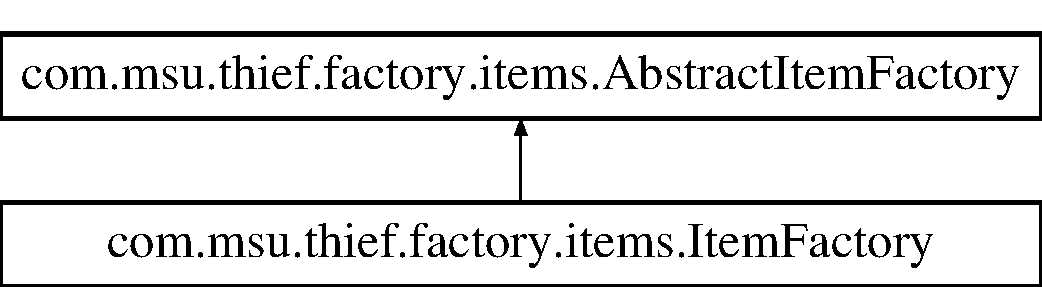
\includegraphics[height=2.000000cm]{classcom_1_1msu_1_1thief_1_1factory_1_1items_1_1ItemFactory}
\end{center}
\end{figure}
\subsection*{Classes}
\begin{DoxyCompactItemize}
\item 
enum {\bfseries C\-O\-R\-R\-E\-L\-A\-T\-I\-O\-N\-\_\-\-T\-Y\-P\-E}
\end{DoxyCompactItemize}
\subsection*{Public Member Functions}
\begin{DoxyCompactItemize}
\item 
\hypertarget{classcom_1_1msu_1_1thief_1_1factory_1_1items_1_1ItemFactory_a24b89b712a6694887a00f5f739e4b5f9}{{\bfseries Item\-Factory} (C\-O\-R\-R\-E\-L\-A\-T\-I\-O\-N\-\_\-\-T\-Y\-P\-E corr\-Type)}\label{classcom_1_1msu_1_1thief_1_1factory_1_1items_1_1ItemFactory_a24b89b712a6694887a00f5f739e4b5f9}

\item 
\hypertarget{classcom_1_1msu_1_1thief_1_1factory_1_1items_1_1ItemFactory_a33d74d9431b732cd3125cf09bfd11f3d}{{\bfseries Item\-Factory} (C\-O\-R\-R\-E\-L\-A\-T\-I\-O\-N\-\_\-\-T\-Y\-P\-E corr\-Type, int maximal\-Value)}\label{classcom_1_1msu_1_1thief_1_1factory_1_1items_1_1ItemFactory_a33d74d9431b732cd3125cf09bfd11f3d}

\item 
\hypertarget{classcom_1_1msu_1_1thief_1_1factory_1_1items_1_1ItemFactory_a900604a0607b6a7f420c92c55b70bd1e}{\hyperlink{classcom_1_1msu_1_1thief_1_1model_1_1Item}{Item} {\bfseries create} ()}\label{classcom_1_1msu_1_1thief_1_1factory_1_1items_1_1ItemFactory_a900604a0607b6a7f420c92c55b70bd1e}

\item 
\hypertarget{classcom_1_1msu_1_1thief_1_1factory_1_1items_1_1ItemFactory_a05d9d49b785a3e97c0242e115f4ebfea}{int {\bfseries get\-Maximal\-Value} ()}\label{classcom_1_1msu_1_1thief_1_1factory_1_1items_1_1ItemFactory_a05d9d49b785a3e97c0242e115f4ebfea}

\item 
\hypertarget{classcom_1_1msu_1_1thief_1_1factory_1_1items_1_1ItemFactory_a0ffeadc85b4a9e0f61ca4a4b7c4adf48}{void {\bfseries set\-Maximal\-Value} (int maximal\-Value)}\label{classcom_1_1msu_1_1thief_1_1factory_1_1items_1_1ItemFactory_a0ffeadc85b4a9e0f61ca4a4b7c4adf48}

\item 
\hypertarget{classcom_1_1msu_1_1thief_1_1factory_1_1items_1_1ItemFactory_aa74023627934a36042ed1871255fbfaa}{C\-O\-R\-R\-E\-L\-A\-T\-I\-O\-N\-\_\-\-T\-Y\-P\-E {\bfseries get\-Corr\-Type} ()}\label{classcom_1_1msu_1_1thief_1_1factory_1_1items_1_1ItemFactory_aa74023627934a36042ed1871255fbfaa}

\item 
\hypertarget{classcom_1_1msu_1_1thief_1_1factory_1_1items_1_1ItemFactory_a9ca4d3562044df5d2657acc35d0a842b}{void {\bfseries set\-Corr\-Type} (C\-O\-R\-R\-E\-L\-A\-T\-I\-O\-N\-\_\-\-T\-Y\-P\-E corr\-Type)}\label{classcom_1_1msu_1_1thief_1_1factory_1_1items_1_1ItemFactory_a9ca4d3562044df5d2657acc35d0a842b}

\item 
\hypertarget{classcom_1_1msu_1_1thief_1_1factory_1_1items_1_1ItemFactory_a8c6da35ca46677994b27e09a1eb49da7}{Double {\bfseries get\-Maximal\-Tour\-Time} ()}\label{classcom_1_1msu_1_1thief_1_1factory_1_1items_1_1ItemFactory_a8c6da35ca46677994b27e09a1eb49da7}

\item 
\hypertarget{classcom_1_1msu_1_1thief_1_1factory_1_1items_1_1ItemFactory_ac31050b1978a7211a43e0c17e1db6663}{void {\bfseries set\-Maximal\-Tour\-Time} (Double maximal\-Tour\-Time)}\label{classcom_1_1msu_1_1thief_1_1factory_1_1items_1_1ItemFactory_ac31050b1978a7211a43e0c17e1db6663}

\end{DoxyCompactItemize}
\subsection*{Static Public Member Functions}
\begin{DoxyCompactItemize}
\item 
\hypertarget{classcom_1_1msu_1_1thief_1_1factory_1_1items_1_1ItemFactory_a36bb709de2fe69d57b53744addac09c2}{static void {\bfseries main} (String\mbox{[}$\,$\mbox{]} args)}\label{classcom_1_1msu_1_1thief_1_1factory_1_1items_1_1ItemFactory_a36bb709de2fe69d57b53744addac09c2}

\end{DoxyCompactItemize}
\subsection*{Protected Attributes}
\begin{DoxyCompactItemize}
\item 
\hypertarget{classcom_1_1msu_1_1thief_1_1factory_1_1items_1_1ItemFactory_a34629798e69390022e74f057fee39b57}{int {\bfseries maximal\-Value} = 1000}\label{classcom_1_1msu_1_1thief_1_1factory_1_1items_1_1ItemFactory_a34629798e69390022e74f057fee39b57}

\item 
\hypertarget{classcom_1_1msu_1_1thief_1_1factory_1_1items_1_1ItemFactory_a042798537b4713fd0fd18a76182d3b50}{C\-O\-R\-R\-E\-L\-A\-T\-I\-O\-N\-\_\-\-T\-Y\-P\-E {\bfseries corr\-Type} = C\-O\-R\-R\-E\-L\-A\-T\-I\-O\-N\-\_\-\-T\-Y\-P\-E.\-U\-N\-C\-O\-R\-R\-E\-L\-A\-T\-E\-D}\label{classcom_1_1msu_1_1thief_1_1factory_1_1items_1_1ItemFactory_a042798537b4713fd0fd18a76182d3b50}

\item 
\hypertarget{classcom_1_1msu_1_1thief_1_1factory_1_1items_1_1ItemFactory_adabff26a1dfbc7af247d140832c75ca7}{Double {\bfseries maximal\-Tour\-Time} = null}\label{classcom_1_1msu_1_1thief_1_1factory_1_1items_1_1ItemFactory_adabff26a1dfbc7af247d140832c75ca7}

\end{DoxyCompactItemize}


The documentation for this class was generated from the following file\-:\begin{DoxyCompactItemize}
\item 
src/main/java/com/msu/thief/factory/items/Item\-Factory.\-java\end{DoxyCompactItemize}

\hypertarget{interfacecom_1_1msu_1_1thief_1_1model_1_1tour_1_1ITourFactory_3_01P_01extends_01ICityProblem_01_4}{\section{com.\-msu.\-thief.\-model.\-tour.\-I\-Tour\-Factory$<$ P extends I\-City\-Problem $>$ Interface Reference}
\label{interfacecom_1_1msu_1_1thief_1_1model_1_1tour_1_1ITourFactory_3_01P_01extends_01ICityProblem_01_4}\index{com.\-msu.\-thief.\-model.\-tour.\-I\-Tour\-Factory$<$ P extends I\-City\-Problem $>$@{com.\-msu.\-thief.\-model.\-tour.\-I\-Tour\-Factory$<$ P extends I\-City\-Problem $>$}}
}
Inheritance diagram for com.\-msu.\-thief.\-model.\-tour.\-I\-Tour\-Factory$<$ P extends I\-City\-Problem $>$\-:\begin{figure}[H]
\begin{center}
\leavevmode
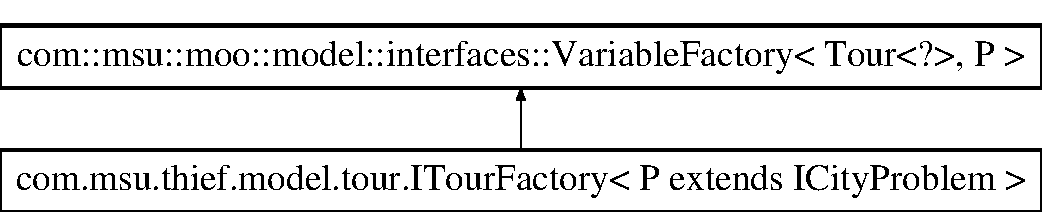
\includegraphics[height=2.000000cm]{interfacecom_1_1msu_1_1thief_1_1model_1_1tour_1_1ITourFactory_3_01P_01extends_01ICityProblem_01_4}
\end{center}
\end{figure}
\subsection*{Public Member Functions}
\begin{DoxyCompactItemize}
\item 
\hypertarget{interfacecom_1_1msu_1_1thief_1_1model_1_1tour_1_1ITourFactory_3_01P_01extends_01ICityProblem_01_4_a0121b64f9ae59e3382d6abe05bbe99cf}{Tour$<$?$>$ {\bfseries create} (P p)}\label{interfacecom_1_1msu_1_1thief_1_1model_1_1tour_1_1ITourFactory_3_01P_01extends_01ICityProblem_01_4_a0121b64f9ae59e3382d6abe05bbe99cf}

\end{DoxyCompactItemize}


The documentation for this interface was generated from the following file\-:\begin{DoxyCompactItemize}
\item 
src/main/java/com/msu/thief/model/tour/I\-Tour\-Factory.\-java\end{DoxyCompactItemize}

\hypertarget{classcom_1_1msu_1_1knp_1_1KnapsackExhaustiveFactory}{\section{com.\-msu.\-knp.\-Knapsack\-Exhaustive\-Factory Class Reference}
\label{classcom_1_1msu_1_1knp_1_1KnapsackExhaustiveFactory}\index{com.\-msu.\-knp.\-Knapsack\-Exhaustive\-Factory@{com.\-msu.\-knp.\-Knapsack\-Exhaustive\-Factory}}
}
Inheritance diagram for com.\-msu.\-knp.\-Knapsack\-Exhaustive\-Factory\-:\begin{figure}[H]
\begin{center}
\leavevmode
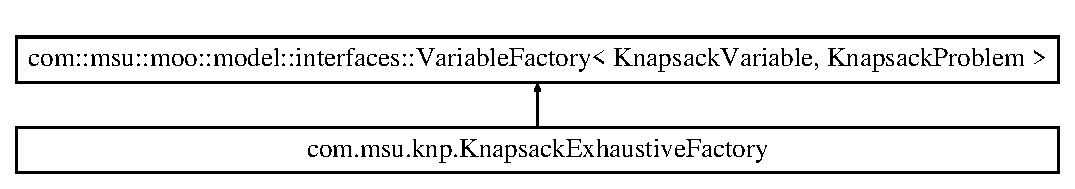
\includegraphics[height=2.000000cm]{classcom_1_1msu_1_1knp_1_1KnapsackExhaustiveFactory}
\end{center}
\end{figure}
\subsection*{Public Member Functions}
\begin{DoxyCompactItemize}
\item 
\hypertarget{classcom_1_1msu_1_1knp_1_1KnapsackExhaustiveFactory_a5e204da3a25b44b428abb0fb592ebffe}{\hyperlink{classcom_1_1msu_1_1knp_1_1KnapsackVariable}{Knapsack\-Variable} {\bfseries create} (\hyperlink{classcom_1_1msu_1_1knp_1_1KnapsackProblem}{Knapsack\-Problem} problem)}\label{classcom_1_1msu_1_1knp_1_1KnapsackExhaustiveFactory_a5e204da3a25b44b428abb0fb592ebffe}

\end{DoxyCompactItemize}
\subsection*{Static Public Member Functions}
\begin{DoxyCompactItemize}
\item 
\hypertarget{classcom_1_1msu_1_1knp_1_1KnapsackExhaustiveFactory_acdbd5e5253450a5717d38d957d079d38}{static void {\bfseries main} (String\mbox{[}$\,$\mbox{]} args)}\label{classcom_1_1msu_1_1knp_1_1KnapsackExhaustiveFactory_acdbd5e5253450a5717d38d957d079d38}

\end{DoxyCompactItemize}
\subsection*{Protected Attributes}
\begin{DoxyCompactItemize}
\item 
\hypertarget{classcom_1_1msu_1_1knp_1_1KnapsackExhaustiveFactory_afb5a77a29446181ea76319057f403d0c}{Queue$<$ List$<$ Boolean $>$ $>$ {\bfseries q} = null}\label{classcom_1_1msu_1_1knp_1_1KnapsackExhaustiveFactory_afb5a77a29446181ea76319057f403d0c}

\end{DoxyCompactItemize}


The documentation for this class was generated from the following file\-:\begin{DoxyCompactItemize}
\item 
src/main/java/com/msu/knp/Knapsack\-Exhaustive\-Factory.\-java\end{DoxyCompactItemize}

\hypertarget{classcom_1_1msu_1_1knp_1_1KnapsackProblem}{\section{com.\-msu.\-knp.\-Knapsack\-Problem Class Reference}
\label{classcom_1_1msu_1_1knp_1_1KnapsackProblem}\index{com.\-msu.\-knp.\-Knapsack\-Problem@{com.\-msu.\-knp.\-Knapsack\-Problem}}
}
Inheritance diagram for com.\-msu.\-knp.\-Knapsack\-Problem\-:\begin{figure}[H]
\begin{center}
\leavevmode
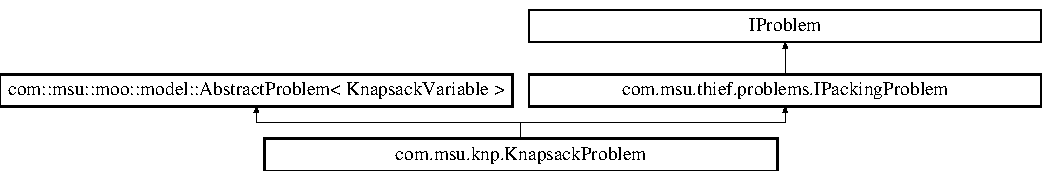
\includegraphics[height=2.301370cm]{classcom_1_1msu_1_1knp_1_1KnapsackProblem}
\end{center}
\end{figure}
\subsection*{Public Member Functions}
\begin{DoxyCompactItemize}
\item 
\hyperlink{classcom_1_1msu_1_1knp_1_1KnapsackProblem_a8cc3eead021b3b28d87be891563fcda3}{Knapsack\-Problem} (int max\-Weight, List$<$ \hyperlink{classcom_1_1msu_1_1thief_1_1model_1_1Item}{Item} $>$ items)
\item 
double \hyperlink{classcom_1_1msu_1_1knp_1_1KnapsackProblem_a688e4bdef229b11397db6c65421228cb}{evaluate} (List$<$ Boolean $>$ b)
\item 
\hypertarget{classcom_1_1msu_1_1knp_1_1KnapsackProblem_a16aa516d8fadcd091124badf0f837526}{int {\bfseries get\-Number\-Of\-Objectives} ()}\label{classcom_1_1msu_1_1knp_1_1KnapsackProblem_a16aa516d8fadcd091124badf0f837526}

\item 
\hypertarget{classcom_1_1msu_1_1knp_1_1KnapsackProblem_afe0445cd0c20ac2c95937d4253770228}{int {\bfseries num\-Of\-Items} ()}\label{classcom_1_1msu_1_1knp_1_1KnapsackProblem_afe0445cd0c20ac2c95937d4253770228}

\end{DoxyCompactItemize}
\subsection*{Static Public Member Functions}
\begin{DoxyCompactItemize}
\item 
\hypertarget{classcom_1_1msu_1_1knp_1_1KnapsackProblem_a001af3c71b70b741fbb9e97be55b0771}{static$<$ Textends\-Item $>$ double {\bfseries get\-Weight} (List$<$ T $>$ items, List$<$ Boolean $>$ b)}\label{classcom_1_1msu_1_1knp_1_1KnapsackProblem_a001af3c71b70b741fbb9e97be55b0771}

\item 
\hypertarget{classcom_1_1msu_1_1knp_1_1KnapsackProblem_a76140b794fa226f6b3cd945bbf717814}{static$<$ Textends\-Item $>$ double {\bfseries get\-Profit} (List$<$ T $>$ items, List$<$ Boolean $>$ b)}\label{classcom_1_1msu_1_1knp_1_1KnapsackProblem_a76140b794fa226f6b3cd945bbf717814}

\item 
static$<$ Textends\-Item $>$ double \hyperlink{classcom_1_1msu_1_1knp_1_1KnapsackProblem_ae82777f42a9c6b80eca15ebc2864cd86}{get\-Sum\-Item\-Attribute} (List$<$ T $>$ items, List$<$ Boolean $>$ b, Function$<$ T, Double $>$ func)
\end{DoxyCompactItemize}
\subsection*{Protected Member Functions}
\begin{DoxyCompactItemize}
\item 
\hypertarget{classcom_1_1msu_1_1knp_1_1KnapsackProblem_adc1b4a49bcd78ca332d993609ec3f0ab}{List$<$ Double $>$ {\bfseries evaluate\-\_\-} (\hyperlink{classcom_1_1msu_1_1knp_1_1KnapsackVariable}{Knapsack\-Variable} variable)}\label{classcom_1_1msu_1_1knp_1_1KnapsackProblem_adc1b4a49bcd78ca332d993609ec3f0ab}

\end{DoxyCompactItemize}


\subsection{Detailed Description}
This class represents the knapsack problem.

The Problem is defined by items that could be added and a maximal weight that fits into the knapsack. 

\subsection{Constructor \& Destructor Documentation}
\hypertarget{classcom_1_1msu_1_1knp_1_1KnapsackProblem_a8cc3eead021b3b28d87be891563fcda3}{\index{com\-::msu\-::knp\-::\-Knapsack\-Problem@{com\-::msu\-::knp\-::\-Knapsack\-Problem}!Knapsack\-Problem@{Knapsack\-Problem}}
\index{Knapsack\-Problem@{Knapsack\-Problem}!com::msu::knp::KnapsackProblem@{com\-::msu\-::knp\-::\-Knapsack\-Problem}}
\subsubsection[{Knapsack\-Problem}]{\setlength{\rightskip}{0pt plus 5cm}com.\-msu.\-knp.\-Knapsack\-Problem.\-Knapsack\-Problem (
\begin{DoxyParamCaption}
\item[{int}]{max\-Weight, }
\item[{List$<$ {\bf Item} $>$}]{items}
\end{DoxyParamCaption}
)\hspace{0.3cm}{\ttfamily [inline]}}}\label{classcom_1_1msu_1_1knp_1_1KnapsackProblem_a8cc3eead021b3b28d87be891563fcda3}
Create a Knapsack Problem with predefined items and a maximal weight!


\begin{DoxyParams}{Parameters}
{\em max\-Weight} & maximal weight of the knapsack \\
\hline
{\em items} & that could be added \\
\hline
\end{DoxyParams}


\subsection{Member Function Documentation}
\hypertarget{classcom_1_1msu_1_1knp_1_1KnapsackProblem_a688e4bdef229b11397db6c65421228cb}{\index{com\-::msu\-::knp\-::\-Knapsack\-Problem@{com\-::msu\-::knp\-::\-Knapsack\-Problem}!evaluate@{evaluate}}
\index{evaluate@{evaluate}!com::msu::knp::KnapsackProblem@{com\-::msu\-::knp\-::\-Knapsack\-Problem}}
\subsubsection[{evaluate}]{\setlength{\rightskip}{0pt plus 5cm}double com.\-msu.\-knp.\-Knapsack\-Problem.\-evaluate (
\begin{DoxyParamCaption}
\item[{List$<$ Boolean $>$}]{b}
\end{DoxyParamCaption}
)\hspace{0.3cm}{\ttfamily [inline]}}}\label{classcom_1_1msu_1_1knp_1_1KnapsackProblem_a688e4bdef229b11397db6c65421228cb}
Evaluate the knapsack problem.


\begin{DoxyParams}{Parameters}
{\em b} & that defines which items to pick \\
\hline
\end{DoxyParams}
\begin{DoxyReturn}{Returns}
the profit of the knapsack 
\end{DoxyReturn}
\hypertarget{classcom_1_1msu_1_1knp_1_1KnapsackProblem_ae82777f42a9c6b80eca15ebc2864cd86}{\index{com\-::msu\-::knp\-::\-Knapsack\-Problem@{com\-::msu\-::knp\-::\-Knapsack\-Problem}!get\-Sum\-Item\-Attribute@{get\-Sum\-Item\-Attribute}}
\index{get\-Sum\-Item\-Attribute@{get\-Sum\-Item\-Attribute}!com::msu::knp::KnapsackProblem@{com\-::msu\-::knp\-::\-Knapsack\-Problem}}
\subsubsection[{get\-Sum\-Item\-Attribute}]{\setlength{\rightskip}{0pt plus 5cm}static $<$Textends\-Item$>$ double com.\-msu.\-knp.\-Knapsack\-Problem.\-get\-Sum\-Item\-Attribute (
\begin{DoxyParamCaption}
\item[{List$<$ T $>$}]{items, }
\item[{List$<$ Boolean $>$}]{b, }
\item[{Function$<$ T, Double $>$}]{func}
\end{DoxyParamCaption}
)\hspace{0.3cm}{\ttfamily [inline]}, {\ttfamily [static]}}}\label{classcom_1_1msu_1_1knp_1_1KnapsackProblem_ae82777f42a9c6b80eca15ebc2864cd86}
Calculate the sum by using a lambda expression


\begin{DoxyParams}{Parameters}
{\em items} & that could be added \\
\hline
{\em b} & for the knapsack \\
\hline
{\em func} & lambda expression \\
\hline
\end{DoxyParams}
\begin{DoxyReturn}{Returns}
resulting weight 
\end{DoxyReturn}


The documentation for this class was generated from the following file\-:\begin{DoxyCompactItemize}
\item 
src/main/java/com/msu/knp/Knapsack\-Problem.\-java\end{DoxyCompactItemize}

\hypertarget{classcom_1_1msu_1_1knp_1_1KnapsackVariable}{\section{com.\-msu.\-knp.\-Knapsack\-Variable Class Reference}
\label{classcom_1_1msu_1_1knp_1_1KnapsackVariable}\index{com.\-msu.\-knp.\-Knapsack\-Variable@{com.\-msu.\-knp.\-Knapsack\-Variable}}
}
Inheritance diagram for com.\-msu.\-knp.\-Knapsack\-Variable\-:\begin{figure}[H]
\begin{center}
\leavevmode
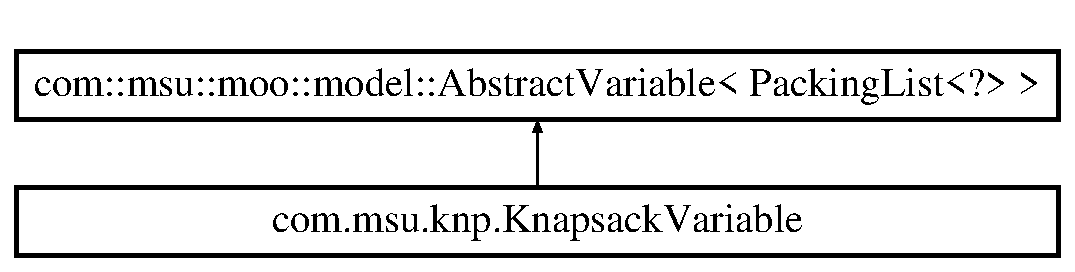
\includegraphics[height=2.000000cm]{classcom_1_1msu_1_1knp_1_1KnapsackVariable}
\end{center}
\end{figure}
\subsection*{Public Member Functions}
\begin{DoxyCompactItemize}
\item 
\hypertarget{classcom_1_1msu_1_1knp_1_1KnapsackVariable_aab3b919cf394606d5fe7a1e5744d43e0}{{\bfseries Knapsack\-Variable} (Packing\-List$<$?$>$ obj)}\label{classcom_1_1msu_1_1knp_1_1KnapsackVariable_aab3b919cf394606d5fe7a1e5744d43e0}

\item 
\hypertarget{classcom_1_1msu_1_1knp_1_1KnapsackVariable_a3b82219f632fa6a63a15790c151d1504}{I\-Variable {\bfseries copy} ()}\label{classcom_1_1msu_1_1knp_1_1KnapsackVariable_a3b82219f632fa6a63a15790c151d1504}

\end{DoxyCompactItemize}


The documentation for this class was generated from the following file\-:\begin{DoxyCompactItemize}
\item 
src/main/java/com/msu/knp/Knapsack\-Variable.\-java\end{DoxyCompactItemize}

\hypertarget{classcom_1_1msu_1_1knp_1_1experiment_1_1KNP__13__1000__1000__1__Experiment}{\section{com.\-msu.\-knp.\-experiment.\-K\-N\-P\-\_\-13\-\_\-1000\-\_\-1000\-\_\-1\-\_\-\-Experiment Class Reference}
\label{classcom_1_1msu_1_1knp_1_1experiment_1_1KNP__13__1000__1000__1__Experiment}\index{com.\-msu.\-knp.\-experiment.\-K\-N\-P\-\_\-13\-\_\-1000\-\_\-1000\-\_\-1\-\_\-\-Experiment@{com.\-msu.\-knp.\-experiment.\-K\-N\-P\-\_\-13\-\_\-1000\-\_\-1000\-\_\-1\-\_\-\-Experiment}}
}
Inheritance diagram for com.\-msu.\-knp.\-experiment.\-K\-N\-P\-\_\-13\-\_\-1000\-\_\-1000\-\_\-1\-\_\-\-Experiment\-:\begin{figure}[H]
\begin{center}
\leavevmode
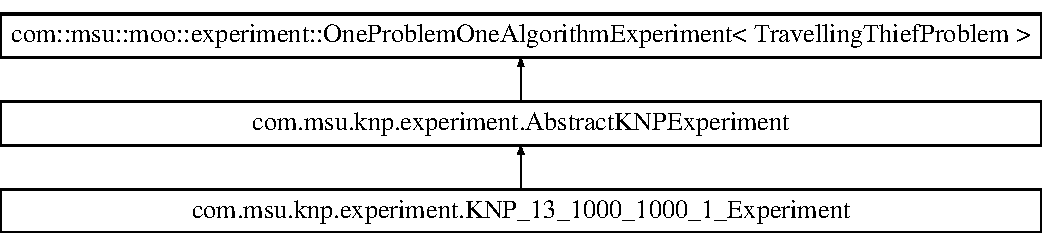
\includegraphics[height=3.000000cm]{classcom_1_1msu_1_1knp_1_1experiment_1_1KNP__13__1000__1000__1__Experiment}
\end{center}
\end{figure}
\subsection*{Protected Member Functions}
\begin{DoxyCompactItemize}
\item 
\hypertarget{classcom_1_1msu_1_1knp_1_1experiment_1_1KNP__13__1000__1000__1__Experiment_a03c2a231cdbf762b238e117a80fa3e7b}{Integer\mbox{[}$\,$\mbox{]}\mbox{[}$\,$\mbox{]} {\bfseries get\-Items} ()}\label{classcom_1_1msu_1_1knp_1_1experiment_1_1KNP__13__1000__1000__1__Experiment_a03c2a231cdbf762b238e117a80fa3e7b}

\item 
\hypertarget{classcom_1_1msu_1_1knp_1_1experiment_1_1KNP__13__1000__1000__1__Experiment_a9ca4349b355a7bbe2ccafd7a03fa02c2}{Integer\mbox{[}$\,$\mbox{]} {\bfseries get\-Optimum} ()}\label{classcom_1_1msu_1_1knp_1_1experiment_1_1KNP__13__1000__1000__1__Experiment_a9ca4349b355a7bbe2ccafd7a03fa02c2}

\item 
\hypertarget{classcom_1_1msu_1_1knp_1_1experiment_1_1KNP__13__1000__1000__1__Experiment_ab572a8d51bd75668b8c666a05383302d}{Integer {\bfseries get\-Max\-Weight} ()}\label{classcom_1_1msu_1_1knp_1_1experiment_1_1KNP__13__1000__1000__1__Experiment_ab572a8d51bd75668b8c666a05383302d}

\end{DoxyCompactItemize}
\subsection*{Additional Inherited Members}


The documentation for this class was generated from the following file\-:\begin{DoxyCompactItemize}
\item 
src/main/java/com/msu/knp/experiment/K\-N\-P\-\_\-13\-\_\-1000\-\_\-1000\-\_\-1\-\_\-\-Experiment.\-java\end{DoxyCompactItemize}

\hypertarget{classcom_1_1msu_1_1knp_1_1experiment_1_1KNP__13__2000__1000__1__Experiment}{\section{com.\-msu.\-knp.\-experiment.\-K\-N\-P\-\_\-13\-\_\-2000\-\_\-1000\-\_\-1\-\_\-\-Experiment Class Reference}
\label{classcom_1_1msu_1_1knp_1_1experiment_1_1KNP__13__2000__1000__1__Experiment}\index{com.\-msu.\-knp.\-experiment.\-K\-N\-P\-\_\-13\-\_\-2000\-\_\-1000\-\_\-1\-\_\-\-Experiment@{com.\-msu.\-knp.\-experiment.\-K\-N\-P\-\_\-13\-\_\-2000\-\_\-1000\-\_\-1\-\_\-\-Experiment}}
}
Inheritance diagram for com.\-msu.\-knp.\-experiment.\-K\-N\-P\-\_\-13\-\_\-2000\-\_\-1000\-\_\-1\-\_\-\-Experiment\-:\begin{figure}[H]
\begin{center}
\leavevmode
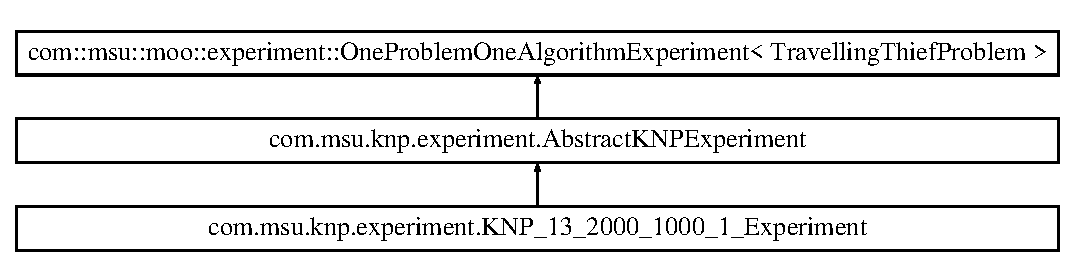
\includegraphics[height=3.000000cm]{classcom_1_1msu_1_1knp_1_1experiment_1_1KNP__13__2000__1000__1__Experiment}
\end{center}
\end{figure}
\subsection*{Protected Member Functions}
\begin{DoxyCompactItemize}
\item 
\hypertarget{classcom_1_1msu_1_1knp_1_1experiment_1_1KNP__13__2000__1000__1__Experiment_a2760560606091ba58ad566a0f6f6cb72}{Integer\mbox{[}$\,$\mbox{]}\mbox{[}$\,$\mbox{]} {\bfseries get\-Items} ()}\label{classcom_1_1msu_1_1knp_1_1experiment_1_1KNP__13__2000__1000__1__Experiment_a2760560606091ba58ad566a0f6f6cb72}

\item 
\hypertarget{classcom_1_1msu_1_1knp_1_1experiment_1_1KNP__13__2000__1000__1__Experiment_a090195441636600405c7d7cd3803cff3}{Integer\mbox{[}$\,$\mbox{]} {\bfseries get\-Optimum} ()}\label{classcom_1_1msu_1_1knp_1_1experiment_1_1KNP__13__2000__1000__1__Experiment_a090195441636600405c7d7cd3803cff3}

\item 
\hypertarget{classcom_1_1msu_1_1knp_1_1experiment_1_1KNP__13__2000__1000__1__Experiment_ae54f4f07c9e3d3e4c92651e96fb734ba}{Integer {\bfseries get\-Max\-Weight} ()}\label{classcom_1_1msu_1_1knp_1_1experiment_1_1KNP__13__2000__1000__1__Experiment_ae54f4f07c9e3d3e4c92651e96fb734ba}

\end{DoxyCompactItemize}
\subsection*{Additional Inherited Members}


The documentation for this class was generated from the following file\-:\begin{DoxyCompactItemize}
\item 
src/main/java/com/msu/knp/experiment/K\-N\-P\-\_\-13\-\_\-2000\-\_\-1000\-\_\-1\-\_\-\-Experiment.\-java\end{DoxyCompactItemize}

\hypertarget{classcom_1_1msu_1_1knp_1_1experiment_1_1KNP__13__200__1000__1__Experiment}{\section{com.\-msu.\-knp.\-experiment.\-K\-N\-P\-\_\-13\-\_\-200\-\_\-1000\-\_\-1\-\_\-\-Experiment Class Reference}
\label{classcom_1_1msu_1_1knp_1_1experiment_1_1KNP__13__200__1000__1__Experiment}\index{com.\-msu.\-knp.\-experiment.\-K\-N\-P\-\_\-13\-\_\-200\-\_\-1000\-\_\-1\-\_\-\-Experiment@{com.\-msu.\-knp.\-experiment.\-K\-N\-P\-\_\-13\-\_\-200\-\_\-1000\-\_\-1\-\_\-\-Experiment}}
}
Inheritance diagram for com.\-msu.\-knp.\-experiment.\-K\-N\-P\-\_\-13\-\_\-200\-\_\-1000\-\_\-1\-\_\-\-Experiment\-:\begin{figure}[H]
\begin{center}
\leavevmode
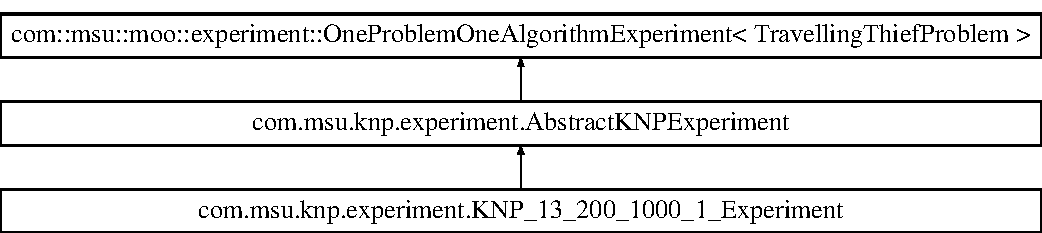
\includegraphics[height=3.000000cm]{classcom_1_1msu_1_1knp_1_1experiment_1_1KNP__13__200__1000__1__Experiment}
\end{center}
\end{figure}
\subsection*{Protected Member Functions}
\begin{DoxyCompactItemize}
\item 
\hypertarget{classcom_1_1msu_1_1knp_1_1experiment_1_1KNP__13__200__1000__1__Experiment_a3ba9746feacd9e4146f6043fb69bf9de}{Integer\mbox{[}$\,$\mbox{]}\mbox{[}$\,$\mbox{]} {\bfseries get\-Items} ()}\label{classcom_1_1msu_1_1knp_1_1experiment_1_1KNP__13__200__1000__1__Experiment_a3ba9746feacd9e4146f6043fb69bf9de}

\item 
\hypertarget{classcom_1_1msu_1_1knp_1_1experiment_1_1KNP__13__200__1000__1__Experiment_a29e2e186e96914ec9ca63b65d13b65bd}{Integer\mbox{[}$\,$\mbox{]} {\bfseries get\-Optimum} ()}\label{classcom_1_1msu_1_1knp_1_1experiment_1_1KNP__13__200__1000__1__Experiment_a29e2e186e96914ec9ca63b65d13b65bd}

\item 
\hypertarget{classcom_1_1msu_1_1knp_1_1experiment_1_1KNP__13__200__1000__1__Experiment_af89e35b989f854ee3f6798c3d69c4209}{Integer {\bfseries get\-Max\-Weight} ()}\label{classcom_1_1msu_1_1knp_1_1experiment_1_1KNP__13__200__1000__1__Experiment_af89e35b989f854ee3f6798c3d69c4209}

\end{DoxyCompactItemize}
\subsection*{Additional Inherited Members}


The documentation for this class was generated from the following file\-:\begin{DoxyCompactItemize}
\item 
src/main/java/com/msu/knp/experiment/K\-N\-P\-\_\-13\-\_\-200\-\_\-1000\-\_\-1\-\_\-\-Experiment.\-java\end{DoxyCompactItemize}

\hypertarget{classcom_1_1msu_1_1knp_1_1experiment_1_1KNP__13__20__1000__1__Experiment}{\section{com.\-msu.\-knp.\-experiment.\-K\-N\-P\-\_\-13\-\_\-20\-\_\-1000\-\_\-1\-\_\-\-Experiment Class Reference}
\label{classcom_1_1msu_1_1knp_1_1experiment_1_1KNP__13__20__1000__1__Experiment}\index{com.\-msu.\-knp.\-experiment.\-K\-N\-P\-\_\-13\-\_\-20\-\_\-1000\-\_\-1\-\_\-\-Experiment@{com.\-msu.\-knp.\-experiment.\-K\-N\-P\-\_\-13\-\_\-20\-\_\-1000\-\_\-1\-\_\-\-Experiment}}
}
Inheritance diagram for com.\-msu.\-knp.\-experiment.\-K\-N\-P\-\_\-13\-\_\-20\-\_\-1000\-\_\-1\-\_\-\-Experiment\-:\begin{figure}[H]
\begin{center}
\leavevmode
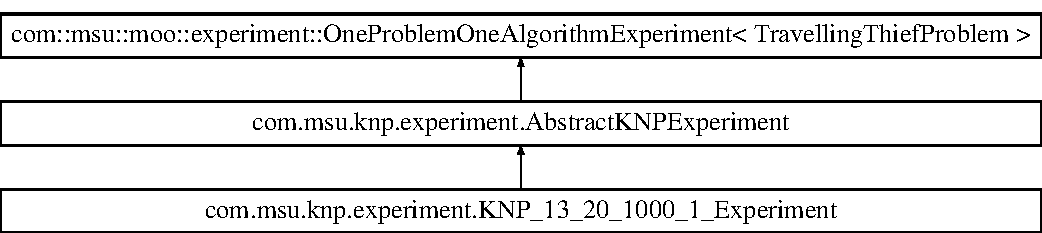
\includegraphics[height=3.000000cm]{classcom_1_1msu_1_1knp_1_1experiment_1_1KNP__13__20__1000__1__Experiment}
\end{center}
\end{figure}
\subsection*{Protected Member Functions}
\begin{DoxyCompactItemize}
\item 
\hypertarget{classcom_1_1msu_1_1knp_1_1experiment_1_1KNP__13__20__1000__1__Experiment_a121904d1b29cfbbff737549879a5b928}{Integer\mbox{[}$\,$\mbox{]}\mbox{[}$\,$\mbox{]} {\bfseries get\-Items} ()}\label{classcom_1_1msu_1_1knp_1_1experiment_1_1KNP__13__20__1000__1__Experiment_a121904d1b29cfbbff737549879a5b928}

\item 
\hypertarget{classcom_1_1msu_1_1knp_1_1experiment_1_1KNP__13__20__1000__1__Experiment_a14fef58c578e8e3c15cee5e02080ac4a}{Integer\mbox{[}$\,$\mbox{]} {\bfseries get\-Optimum} ()}\label{classcom_1_1msu_1_1knp_1_1experiment_1_1KNP__13__20__1000__1__Experiment_a14fef58c578e8e3c15cee5e02080ac4a}

\item 
\hypertarget{classcom_1_1msu_1_1knp_1_1experiment_1_1KNP__13__20__1000__1__Experiment_af5f0209c9c18c7586d4a24a668c38839}{Integer {\bfseries get\-Max\-Weight} ()}\label{classcom_1_1msu_1_1knp_1_1experiment_1_1KNP__13__20__1000__1__Experiment_af5f0209c9c18c7586d4a24a668c38839}

\end{DoxyCompactItemize}
\subsection*{Additional Inherited Members}


The documentation for this class was generated from the following file\-:\begin{DoxyCompactItemize}
\item 
src/main/java/com/msu/knp/experiment/K\-N\-P\-\_\-13\-\_\-20\-\_\-1000\-\_\-1\-\_\-\-Experiment.\-java\end{DoxyCompactItemize}

\hypertarget{classcom_1_1msu_1_1thief_1_1algorithms_1_1LinKernighanHeuristic}{\section{com.\-msu.\-thief.\-algorithms.\-Lin\-Kernighan\-Heuristic Class Reference}
\label{classcom_1_1msu_1_1thief_1_1algorithms_1_1LinKernighanHeuristic}\index{com.\-msu.\-thief.\-algorithms.\-Lin\-Kernighan\-Heuristic@{com.\-msu.\-thief.\-algorithms.\-Lin\-Kernighan\-Heuristic}}
}
Inheritance diagram for com.\-msu.\-thief.\-algorithms.\-Lin\-Kernighan\-Heuristic\-:\begin{figure}[H]
\begin{center}
\leavevmode
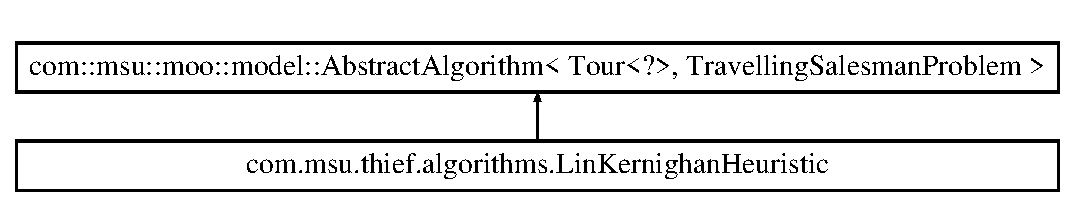
\includegraphics[height=2.000000cm]{classcom_1_1msu_1_1thief_1_1algorithms_1_1LinKernighanHeuristic}
\end{center}
\end{figure}
\subsection*{Public Member Functions}
\begin{DoxyCompactItemize}
\item 
\hypertarget{classcom_1_1msu_1_1thief_1_1algorithms_1_1LinKernighanHeuristic_ae3ac277ba720e435374f5f0172634295}{boolean {\bfseries has\-Finished} ()}\label{classcom_1_1msu_1_1thief_1_1algorithms_1_1LinKernighanHeuristic_ae3ac277ba720e435374f5f0172634295}

\end{DoxyCompactItemize}
\subsection*{Protected Member Functions}
\begin{DoxyCompactItemize}
\item 
\hypertarget{classcom_1_1msu_1_1thief_1_1algorithms_1_1LinKernighanHeuristic_aef8fbed61bf6ab11bf5d8522b8ed401b}{void {\bfseries next} ()}\label{classcom_1_1msu_1_1thief_1_1algorithms_1_1LinKernighanHeuristic_aef8fbed61bf6ab11bf5d8522b8ed401b}

\item 
\hypertarget{classcom_1_1msu_1_1thief_1_1algorithms_1_1LinKernighanHeuristic_ab00c3b797dd4722cf682f05ead593661}{Non\-Dominated\-Solution\-Set {\bfseries get\-Result} ()}\label{classcom_1_1msu_1_1thief_1_1algorithms_1_1LinKernighanHeuristic_ab00c3b797dd4722cf682f05ead593661}

\end{DoxyCompactItemize}
\subsection*{Protected Attributes}
\begin{DoxyCompactItemize}
\item 
\hypertarget{classcom_1_1msu_1_1thief_1_1algorithms_1_1LinKernighanHeuristic_aed44e2908fc11d4667e59e1c495367b6}{String {\bfseries path\-To\-L\-K\-H} = \char`\"{}vendor/L\-K\-H-\/2.\-0.\-7/L\-K\-H\char`\"{}}\label{classcom_1_1msu_1_1thief_1_1algorithms_1_1LinKernighanHeuristic_aed44e2908fc11d4667e59e1c495367b6}

\item 
\hypertarget{classcom_1_1msu_1_1thief_1_1algorithms_1_1LinKernighanHeuristic_a69abbf13ef9b90341f669d787ea97682}{boolean {\bfseries has\-Finished} = false}\label{classcom_1_1msu_1_1thief_1_1algorithms_1_1LinKernighanHeuristic_a69abbf13ef9b90341f669d787ea97682}

\item 
\hypertarget{classcom_1_1msu_1_1thief_1_1algorithms_1_1LinKernighanHeuristic_a645f83bba743a10eb8ba7dc721a80ea4}{List$<$ Integer $>$ {\bfseries result} = null}\label{classcom_1_1msu_1_1thief_1_1algorithms_1_1LinKernighanHeuristic_a645f83bba743a10eb8ba7dc721a80ea4}

\end{DoxyCompactItemize}


\subsection{Detailed Description}
\href{http://www.akira.ruc.dk/~keld/research/LKH/}{\tt http\-://www.\-akira.\-ruc.\-dk/$\sim$keld/research/\-L\-K\-H/}

L\-K\-H is an effective implementation of the Lin-\/\-Kernighan heuristic for solving the traveling salesman problem.

Computational experiments have shown that L\-K\-H is highly effective. Even though the algorithm is approximate, optimal solutions are produced with an impressively high frequency. L\-K\-H has produced optimal solutions for all solved problems we have been able to obtain; including a 85,900-\/city instance (at the time of writing, the largest nontrivial instance solved to optimality). Furthermore, the algorithm has improved the best known solutions for a series of large-\/scale instances with unknown optima, among these a 1,904,711-\/city instance (World T\-S\-P). 

The documentation for this class was generated from the following file\-:\begin{DoxyCompactItemize}
\item 
src/main/java/com/msu/thief/algorithms/Lin\-Kernighan\-Heuristic.\-java\end{DoxyCompactItemize}

\hypertarget{classcom_1_1msu_1_1thief_1_1factory_1_1map_1_1MapFactory}{\section{com.\-msu.\-thief.\-factory.\-map.\-Map\-Factory Class Reference}
\label{classcom_1_1msu_1_1thief_1_1factory_1_1map_1_1MapFactory}\index{com.\-msu.\-thief.\-factory.\-map.\-Map\-Factory@{com.\-msu.\-thief.\-factory.\-map.\-Map\-Factory}}
}
Inheritance diagram for com.\-msu.\-thief.\-factory.\-map.\-Map\-Factory\-:\begin{figure}[H]
\begin{center}
\leavevmode
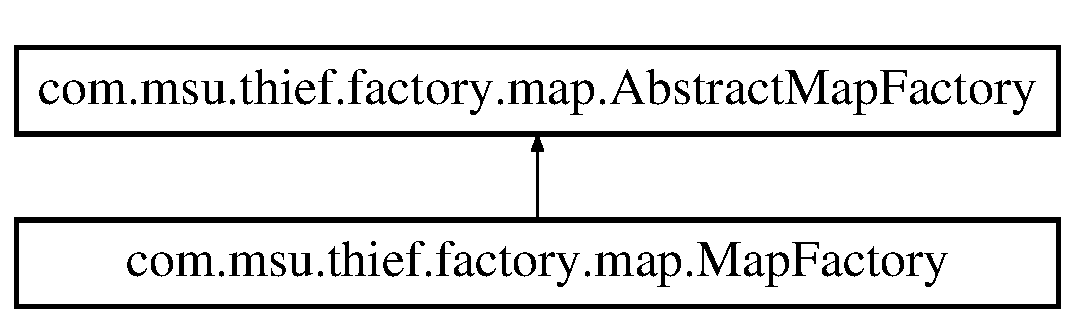
\includegraphics[height=2.000000cm]{classcom_1_1msu_1_1thief_1_1factory_1_1map_1_1MapFactory}
\end{center}
\end{figure}
\subsection*{Classes}
\begin{DoxyCompactItemize}
\item 
enum {\bfseries T\-Y\-P\-E}
\end{DoxyCompactItemize}
\subsection*{Public Member Functions}
\begin{DoxyCompactItemize}
\item 
\hypertarget{classcom_1_1msu_1_1thief_1_1factory_1_1map_1_1MapFactory_a5c1488615b0e4591715fbb04f08f9f1e}{{\bfseries Map\-Factory} (int maximal\-Value)}\label{classcom_1_1msu_1_1thief_1_1factory_1_1map_1_1MapFactory_a5c1488615b0e4591715fbb04f08f9f1e}

\item 
\hypertarget{classcom_1_1msu_1_1thief_1_1factory_1_1map_1_1MapFactory_a49568f42b262a969c1e68b2210e6ca36}{\hyperlink{classcom_1_1msu_1_1thief_1_1model_1_1SymmetricMap}{Symmetric\-Map} {\bfseries create\-From\-Double} (List$<$ Point2\-D $>$ cities)}\label{classcom_1_1msu_1_1thief_1_1factory_1_1map_1_1MapFactory_a49568f42b262a969c1e68b2210e6ca36}

\item 
\hypertarget{classcom_1_1msu_1_1thief_1_1factory_1_1map_1_1MapFactory_aeef2c55f1b39b51f9f975d2d3dc5f35d}{\hyperlink{classcom_1_1msu_1_1thief_1_1model_1_1SymmetricMap}{Symmetric\-Map} {\bfseries create} (List$<$ Point $>$ cities)}\label{classcom_1_1msu_1_1thief_1_1factory_1_1map_1_1MapFactory_aeef2c55f1b39b51f9f975d2d3dc5f35d}

\item 
\hypertarget{classcom_1_1msu_1_1thief_1_1factory_1_1map_1_1MapFactory_a77012b17af6760dc740f4ed8d58f2e9b}{\hyperlink{classcom_1_1msu_1_1thief_1_1model_1_1SymmetricMap}{Symmetric\-Map} {\bfseries create} (int n)}\label{classcom_1_1msu_1_1thief_1_1factory_1_1map_1_1MapFactory_a77012b17af6760dc740f4ed8d58f2e9b}

\item 
\hypertarget{classcom_1_1msu_1_1thief_1_1factory_1_1map_1_1MapFactory_a15e3c92a133fad8a8905dc6782404f65}{T\-Y\-P\-E {\bfseries get\-Type} ()}\label{classcom_1_1msu_1_1thief_1_1factory_1_1map_1_1MapFactory_a15e3c92a133fad8a8905dc6782404f65}

\item 
\hypertarget{classcom_1_1msu_1_1thief_1_1factory_1_1map_1_1MapFactory_abf65e43f6ef59a0c0cb79a1f72546049}{void {\bfseries set\-Type} (T\-Y\-P\-E type)}\label{classcom_1_1msu_1_1thief_1_1factory_1_1map_1_1MapFactory_abf65e43f6ef59a0c0cb79a1f72546049}

\end{DoxyCompactItemize}
\subsection*{Protected Attributes}
\begin{DoxyCompactItemize}
\item 
\hypertarget{classcom_1_1msu_1_1thief_1_1factory_1_1map_1_1MapFactory_a12458983d91830827e50c905eab68f28}{T\-Y\-P\-E {\bfseries type} = T\-Y\-P\-E.\-E\-U\-C\-L\-\_\-2\-D}\label{classcom_1_1msu_1_1thief_1_1factory_1_1map_1_1MapFactory_a12458983d91830827e50c905eab68f28}

\item 
\hypertarget{classcom_1_1msu_1_1thief_1_1factory_1_1map_1_1MapFactory_ac7309f2672343f79be446d8cfedb31aa}{int {\bfseries maximal\-Value} = 1000}\label{classcom_1_1msu_1_1thief_1_1factory_1_1map_1_1MapFactory_ac7309f2672343f79be446d8cfedb31aa}

\item 
\hypertarget{classcom_1_1msu_1_1thief_1_1factory_1_1map_1_1MapFactory_aa8c6ddd8ed78d65d2870819e6b7b96f3}{Random {\bfseries rnd} = Random.\-get\-Instance()}\label{classcom_1_1msu_1_1thief_1_1factory_1_1map_1_1MapFactory_aa8c6ddd8ed78d65d2870819e6b7b96f3}

\end{DoxyCompactItemize}


\subsection{Detailed Description}
This class is used to create a Map which only contains a cost matrix. There is a Map with different points (2\-D with X and Y values) and the euclidean distance between this points is used as a edge cost value. 

The documentation for this class was generated from the following file\-:\begin{DoxyCompactItemize}
\item 
src/main/java/com/msu/thief/factory/map/Map\-Factory.\-java\end{DoxyCompactItemize}

\hypertarget{classcom_1_1msu_1_1thief_1_1evaluator_1_1profit_1_1NoDroppingEvaluator}{\section{com.\-msu.\-thief.\-evaluator.\-profit.\-No\-Dropping\-Evaluator Class Reference}
\label{classcom_1_1msu_1_1thief_1_1evaluator_1_1profit_1_1NoDroppingEvaluator}\index{com.\-msu.\-thief.\-evaluator.\-profit.\-No\-Dropping\-Evaluator@{com.\-msu.\-thief.\-evaluator.\-profit.\-No\-Dropping\-Evaluator}}
}
Inheritance diagram for com.\-msu.\-thief.\-evaluator.\-profit.\-No\-Dropping\-Evaluator\-:\begin{figure}[H]
\begin{center}
\leavevmode
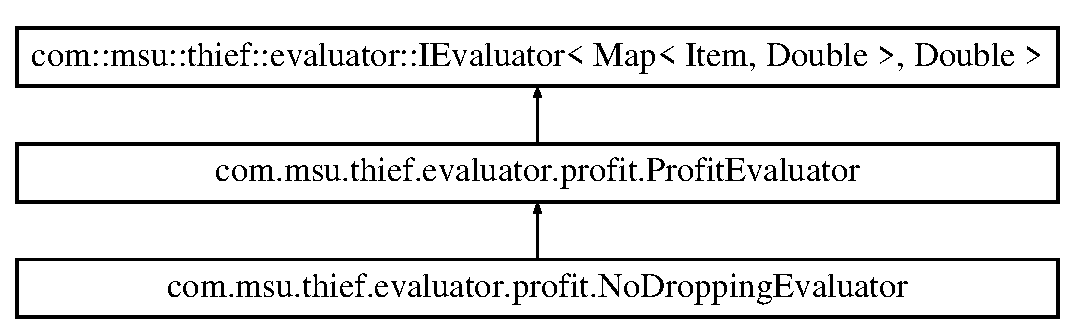
\includegraphics[height=3.000000cm]{classcom_1_1msu_1_1thief_1_1evaluator_1_1profit_1_1NoDroppingEvaluator}
\end{center}
\end{figure}
\subsection*{Public Member Functions}
\begin{DoxyCompactItemize}
\item 
\hypertarget{classcom_1_1msu_1_1thief_1_1evaluator_1_1profit_1_1NoDroppingEvaluator_a3fc1bbaf97937ebb2c8692147473773b}{Double {\bfseries evaluate} (Map$<$ \hyperlink{classcom_1_1msu_1_1thief_1_1model_1_1Item}{Item}, Double $>$ m\-Items)}\label{classcom_1_1msu_1_1thief_1_1evaluator_1_1profit_1_1NoDroppingEvaluator_a3fc1bbaf97937ebb2c8692147473773b}

\end{DoxyCompactItemize}


\subsection{Detailed Description}
The Individual\-Profit\-Calculator calculates the profit by using a dropping rate for each item! 

The documentation for this class was generated from the following file\-:\begin{DoxyCompactItemize}
\item 
src/main/java/com/msu/thief/evaluator/profit/No\-Dropping\-Evaluator.\-java\end{DoxyCompactItemize}

\hypertarget{classcom_1_1msu_1_1thief_1_1evaluator_1_1time_1_1NotBackHomeTimeEvaluator}{\section{com.\-msu.\-thief.\-evaluator.\-time.\-Not\-Back\-Home\-Time\-Evaluator Class Reference}
\label{classcom_1_1msu_1_1thief_1_1evaluator_1_1time_1_1NotBackHomeTimeEvaluator}\index{com.\-msu.\-thief.\-evaluator.\-time.\-Not\-Back\-Home\-Time\-Evaluator@{com.\-msu.\-thief.\-evaluator.\-time.\-Not\-Back\-Home\-Time\-Evaluator}}
}
Inheritance diagram for com.\-msu.\-thief.\-evaluator.\-time.\-Not\-Back\-Home\-Time\-Evaluator\-:\begin{figure}[H]
\begin{center}
\leavevmode
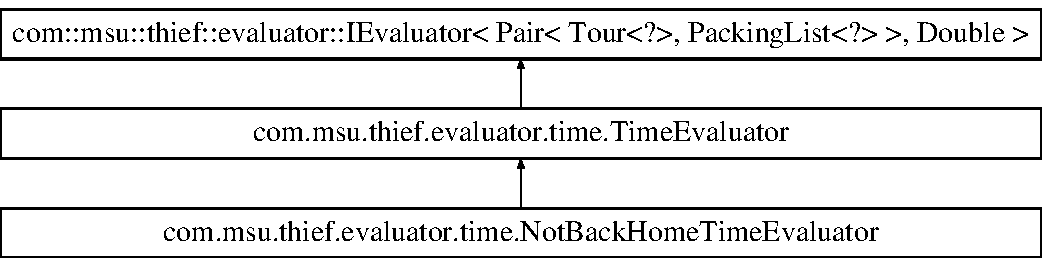
\includegraphics[height=3.000000cm]{classcom_1_1msu_1_1thief_1_1evaluator_1_1time_1_1NotBackHomeTimeEvaluator}
\end{center}
\end{figure}
\subsection*{Public Member Functions}
\begin{DoxyCompactItemize}
\item 
\hypertarget{classcom_1_1msu_1_1thief_1_1evaluator_1_1time_1_1NotBackHomeTimeEvaluator_a4bde4e2a433ddfe6df8f819516a9e05d}{{\bfseries Not\-Back\-Home\-Time\-Evaluator} (\hyperlink{classcom_1_1msu_1_1thief_1_1problems_1_1TravellingThiefProblem}{Travelling\-Thief\-Problem} problem)}\label{classcom_1_1msu_1_1thief_1_1evaluator_1_1time_1_1NotBackHomeTimeEvaluator_a4bde4e2a433ddfe6df8f819516a9e05d}

\item 
\hypertarget{classcom_1_1msu_1_1thief_1_1evaluator_1_1time_1_1NotBackHomeTimeEvaluator_aabf9b6b0a4c551a17bf0e768405ea8c6}{Double {\bfseries evaluate\-\_\-} (Pair$<$ Tour$<$?$>$, Packing\-List$<$?$>$$>$ input)}\label{classcom_1_1msu_1_1thief_1_1evaluator_1_1time_1_1NotBackHomeTimeEvaluator_aabf9b6b0a4c551a17bf0e768405ea8c6}

\end{DoxyCompactItemize}
\subsection*{Additional Inherited Members}


The documentation for this class was generated from the following file\-:\begin{DoxyCompactItemize}
\item 
src/main/java/com/msu/thief/evaluator/time/Not\-Back\-Home\-Time\-Evaluator.\-java\end{DoxyCompactItemize}

\hypertarget{classcom_1_1msu_1_1thief_1_1experiment_1_1NSGAIIOperatorExperiment}{\section{com.\-msu.\-thief.\-experiment.\-N\-S\-G\-A\-I\-I\-Operator\-Experiment Class Reference}
\label{classcom_1_1msu_1_1thief_1_1experiment_1_1NSGAIIOperatorExperiment}\index{com.\-msu.\-thief.\-experiment.\-N\-S\-G\-A\-I\-I\-Operator\-Experiment@{com.\-msu.\-thief.\-experiment.\-N\-S\-G\-A\-I\-I\-Operator\-Experiment}}
}
Inheritance diagram for com.\-msu.\-thief.\-experiment.\-N\-S\-G\-A\-I\-I\-Operator\-Experiment\-:\begin{figure}[H]
\begin{center}
\leavevmode
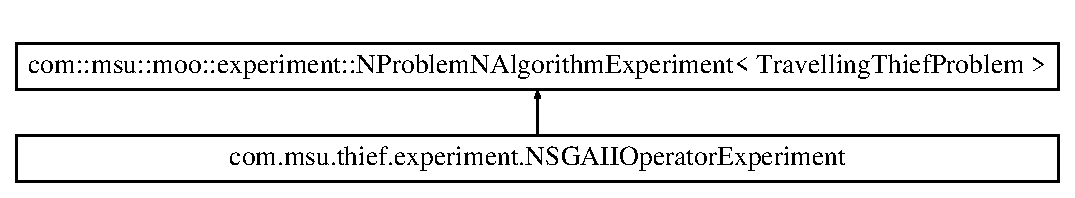
\includegraphics[height=2.000000cm]{classcom_1_1msu_1_1thief_1_1experiment_1_1NSGAIIOperatorExperiment}
\end{center}
\end{figure}
\subsection*{Protected Member Functions}
\begin{DoxyCompactItemize}
\item 
\hypertarget{classcom_1_1msu_1_1thief_1_1experiment_1_1NSGAIIOperatorExperiment_a24ce271b7118ae4650da4115770d4c06}{List$<$ I\-Algorithm\\*
$<$ \hyperlink{classcom_1_1msu_1_1thief_1_1problems_1_1TravellingThiefProblem}{Travelling\-Thief\-Problem} $>$ $>$ {\bfseries get\-Algorithms} ()}\label{classcom_1_1msu_1_1thief_1_1experiment_1_1NSGAIIOperatorExperiment_a24ce271b7118ae4650da4115770d4c06}

\item 
\hypertarget{classcom_1_1msu_1_1thief_1_1experiment_1_1NSGAIIOperatorExperiment_a929ebb8c067bcad09c305c8aa1c93996}{Map$<$ \hyperlink{classcom_1_1msu_1_1thief_1_1problems_1_1TravellingThiefProblem}{Travelling\-Thief\-Problem}, \\*
Non\-Dominated\-Solution\-Set $>$ {\bfseries get\-Problems} ()}\label{classcom_1_1msu_1_1thief_1_1experiment_1_1NSGAIIOperatorExperiment_a929ebb8c067bcad09c305c8aa1c93996}

\end{DoxyCompactItemize}


The documentation for this class was generated from the following file\-:\begin{DoxyCompactItemize}
\item 
src/main/java/com/msu/thief/experiment/N\-S\-G\-A\-I\-I\-Operator\-Experiment.\-java\end{DoxyCompactItemize}

\hypertarget{classcom_1_1msu_1_1thief_1_1experiment_1_1OneScenarioTSPColoredExperiment}{\section{com.\-msu.\-thief.\-experiment.\-One\-Scenario\-T\-S\-P\-Colored\-Experiment Class Reference}
\label{classcom_1_1msu_1_1thief_1_1experiment_1_1OneScenarioTSPColoredExperiment}\index{com.\-msu.\-thief.\-experiment.\-One\-Scenario\-T\-S\-P\-Colored\-Experiment@{com.\-msu.\-thief.\-experiment.\-One\-Scenario\-T\-S\-P\-Colored\-Experiment}}
}
Inheritance diagram for com.\-msu.\-thief.\-experiment.\-One\-Scenario\-T\-S\-P\-Colored\-Experiment\-:\begin{figure}[H]
\begin{center}
\leavevmode
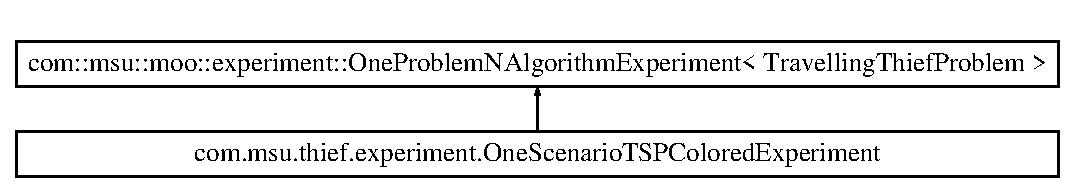
\includegraphics[height=2.000000cm]{classcom_1_1msu_1_1thief_1_1experiment_1_1OneScenarioTSPColoredExperiment}
\end{center}
\end{figure}
\subsection*{Public Member Functions}
\begin{DoxyCompactItemize}
\item 
\hypertarget{classcom_1_1msu_1_1thief_1_1experiment_1_1OneScenarioTSPColoredExperiment_aee1023321c1847259f1f1b9fbfb434ed}{void {\bfseries report} ()}\label{classcom_1_1msu_1_1thief_1_1experiment_1_1OneScenarioTSPColoredExperiment_aee1023321c1847259f1f1b9fbfb434ed}

\end{DoxyCompactItemize}
\subsection*{Protected Member Functions}
\begin{DoxyCompactItemize}
\item 
\hypertarget{classcom_1_1msu_1_1thief_1_1experiment_1_1OneScenarioTSPColoredExperiment_a5e012ded17bc520c2c51ef663004429e}{\hyperlink{classcom_1_1msu_1_1thief_1_1problems_1_1TravellingThiefProblem}{Travelling\-Thief\-Problem} {\bfseries get\-Problem} ()}\label{classcom_1_1msu_1_1thief_1_1experiment_1_1OneScenarioTSPColoredExperiment_a5e012ded17bc520c2c51ef663004429e}

\item 
\hypertarget{classcom_1_1msu_1_1thief_1_1experiment_1_1OneScenarioTSPColoredExperiment_a185d64989e65fe2182c809f92c3fbccb}{Non\-Dominated\-Solution\-Set {\bfseries get\-True\-Front} ()}\label{classcom_1_1msu_1_1thief_1_1experiment_1_1OneScenarioTSPColoredExperiment_a185d64989e65fe2182c809f92c3fbccb}

\item 
\hypertarget{classcom_1_1msu_1_1thief_1_1experiment_1_1OneScenarioTSPColoredExperiment_a534b72a05996c4640e8c7c607b2b75ee}{List$<$ I\-Algorithm\\*
$<$ \hyperlink{classcom_1_1msu_1_1thief_1_1problems_1_1TravellingThiefProblem}{Travelling\-Thief\-Problem} $>$ $>$ {\bfseries get\-Algorithms} ()}\label{classcom_1_1msu_1_1thief_1_1experiment_1_1OneScenarioTSPColoredExperiment_a534b72a05996c4640e8c7c607b2b75ee}

\end{DoxyCompactItemize}


The documentation for this class was generated from the following file\-:\begin{DoxyCompactItemize}
\item 
src/main/java/com/msu/thief/experiment/One\-Scenario\-T\-S\-P\-Colored\-Experiment.\-java\end{DoxyCompactItemize}

\hypertarget{classcom_1_1msu_1_1thief_1_1model_1_1packing_1_1PackingList_3_01T_01_4}{\section{com.\-msu.\-thief.\-model.\-packing.\-Packing\-List$<$ T $>$ Class Reference}
\label{classcom_1_1msu_1_1thief_1_1model_1_1packing_1_1PackingList_3_01T_01_4}\index{com.\-msu.\-thief.\-model.\-packing.\-Packing\-List$<$ T $>$@{com.\-msu.\-thief.\-model.\-packing.\-Packing\-List$<$ T $>$}}
}
Inheritance diagram for com.\-msu.\-thief.\-model.\-packing.\-Packing\-List$<$ T $>$\-:\begin{figure}[H]
\begin{center}
\leavevmode
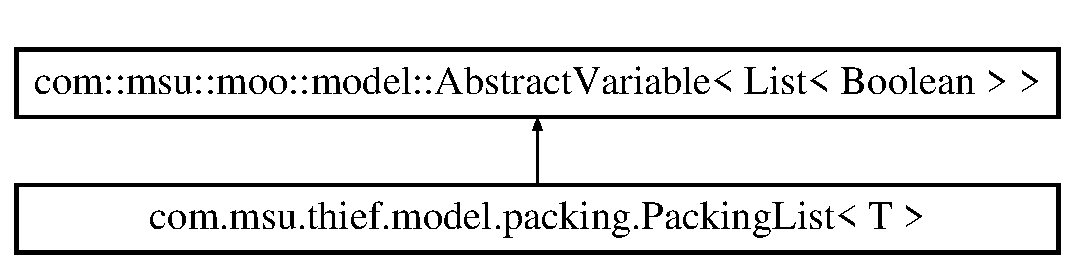
\includegraphics[height=2.000000cm]{classcom_1_1msu_1_1thief_1_1model_1_1packing_1_1PackingList_3_01T_01_4}
\end{center}
\end{figure}
\subsection*{Public Member Functions}
\begin{DoxyCompactItemize}
\item 
\hypertarget{classcom_1_1msu_1_1thief_1_1model_1_1packing_1_1PackingList_3_01T_01_4_a033c53747cd5c19ac7753980f22adb76}{{\bfseries Packing\-List} (List$<$ Boolean $>$ obj)}\label{classcom_1_1msu_1_1thief_1_1model_1_1packing_1_1PackingList_3_01T_01_4_a033c53747cd5c19ac7753980f22adb76}

\item 
\hypertarget{classcom_1_1msu_1_1thief_1_1model_1_1packing_1_1PackingList_3_01T_01_4_afa71557bc36cdb0c05e858841c49c13e}{String {\bfseries to\-String} ()}\label{classcom_1_1msu_1_1thief_1_1model_1_1packing_1_1PackingList_3_01T_01_4_afa71557bc36cdb0c05e858841c49c13e}

\item 
\hypertarget{classcom_1_1msu_1_1thief_1_1model_1_1packing_1_1PackingList_3_01T_01_4_abee72a5b03d4d5fa840e96ce6a162d30}{abstract List$<$ Boolean $>$ {\bfseries encode} ()}\label{classcom_1_1msu_1_1thief_1_1model_1_1packing_1_1PackingList_3_01T_01_4_abee72a5b03d4d5fa840e96ce6a162d30}

\end{DoxyCompactItemize}


The documentation for this class was generated from the following file\-:\begin{DoxyCompactItemize}
\item 
src/main/java/com/msu/thief/model/packing/Packing\-List.\-java\end{DoxyCompactItemize}

\hypertarget{classcom_1_1msu_1_1thief_1_1model_1_1tour_1_1PositionDecodedTour}{\section{com.\-msu.\-thief.\-model.\-tour.\-Position\-Decoded\-Tour Class Reference}
\label{classcom_1_1msu_1_1thief_1_1model_1_1tour_1_1PositionDecodedTour}\index{com.\-msu.\-thief.\-model.\-tour.\-Position\-Decoded\-Tour@{com.\-msu.\-thief.\-model.\-tour.\-Position\-Decoded\-Tour}}
}
Inheritance diagram for com.\-msu.\-thief.\-model.\-tour.\-Position\-Decoded\-Tour\-:\begin{figure}[H]
\begin{center}
\leavevmode
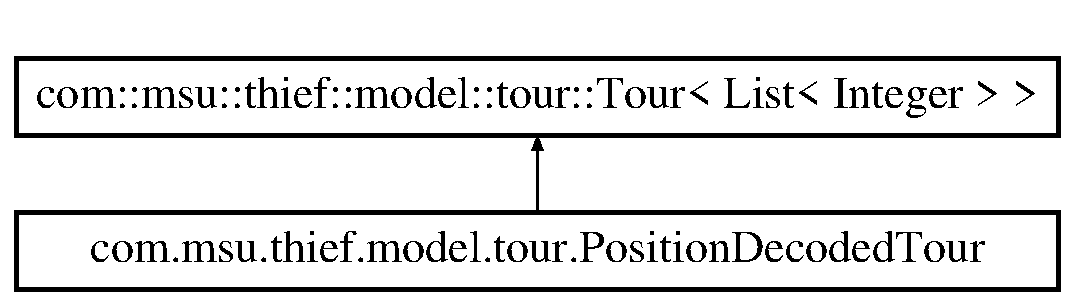
\includegraphics[height=2.000000cm]{classcom_1_1msu_1_1thief_1_1model_1_1tour_1_1PositionDecodedTour}
\end{center}
\end{figure}
\subsection*{Public Member Functions}
\begin{DoxyCompactItemize}
\item 
\hyperlink{classcom_1_1msu_1_1thief_1_1model_1_1tour_1_1PositionDecodedTour_ab54d9954655abe66c783c09b819f5ab1}{Position\-Decoded\-Tour} (List$<$ Integer $>$ list)
\item 
\hypertarget{classcom_1_1msu_1_1thief_1_1model_1_1tour_1_1PositionDecodedTour_afc4625da94122b54f478d4f58de3202a}{\hyperlink{classcom_1_1msu_1_1thief_1_1model_1_1tour_1_1PositionDecodedTour}{Position\-Decoded\-Tour} {\bfseries copy} ()}\label{classcom_1_1msu_1_1thief_1_1model_1_1tour_1_1PositionDecodedTour_afc4625da94122b54f478d4f58de3202a}

\item 
\hypertarget{classcom_1_1msu_1_1thief_1_1model_1_1tour_1_1PositionDecodedTour_a65351c900d4dcf685bd4703884297754}{List$<$ Integer $>$ {\bfseries encode} ()}\label{classcom_1_1msu_1_1thief_1_1model_1_1tour_1_1PositionDecodedTour_a65351c900d4dcf685bd4703884297754}

\end{DoxyCompactItemize}


\subsection{Detailed Description}
The \hyperlink{classcom_1_1msu_1_1thief_1_1model_1_1tour_1_1StandardTour}{Standard\-Tour} provides an implementation of a tour that saves directly the permutation array.

The encoding is nothing else than returning the array directly. 

\subsection{Constructor \& Destructor Documentation}
\hypertarget{classcom_1_1msu_1_1thief_1_1model_1_1tour_1_1PositionDecodedTour_ab54d9954655abe66c783c09b819f5ab1}{\index{com\-::msu\-::thief\-::model\-::tour\-::\-Position\-Decoded\-Tour@{com\-::msu\-::thief\-::model\-::tour\-::\-Position\-Decoded\-Tour}!Position\-Decoded\-Tour@{Position\-Decoded\-Tour}}
\index{Position\-Decoded\-Tour@{Position\-Decoded\-Tour}!com::msu::thief::model::tour::PositionDecodedTour@{com\-::msu\-::thief\-::model\-::tour\-::\-Position\-Decoded\-Tour}}
\subsubsection[{Position\-Decoded\-Tour}]{\setlength{\rightskip}{0pt plus 5cm}com.\-msu.\-thief.\-model.\-tour.\-Position\-Decoded\-Tour.\-Position\-Decoded\-Tour (
\begin{DoxyParamCaption}
\item[{List$<$ Integer $>$}]{list}
\end{DoxyParamCaption}
)\hspace{0.3cm}{\ttfamily [inline]}}}\label{classcom_1_1msu_1_1thief_1_1model_1_1tour_1_1PositionDecodedTour_ab54d9954655abe66c783c09b819f5ab1}
Create a Tour using a permutation vector


\begin{DoxyParams}{Parameters}
{\em list} & tour represented by permutation vector \\
\hline
\end{DoxyParams}


The documentation for this class was generated from the following file\-:\begin{DoxyCompactItemize}
\item 
src/main/java/com/msu/thief/model/tour/Position\-Decoded\-Tour.\-java\end{DoxyCompactItemize}

\hypertarget{classcom_1_1msu_1_1thief_1_1model_1_1tour_1_1PositionDecodedTourFactory_3_01P_01extends_01ICityProblem_01_4}{\section{com.\-msu.\-thief.\-model.\-tour.\-Position\-Decoded\-Tour\-Factory$<$ P extends I\-City\-Problem $>$ Class Reference}
\label{classcom_1_1msu_1_1thief_1_1model_1_1tour_1_1PositionDecodedTourFactory_3_01P_01extends_01ICityProblem_01_4}\index{com.\-msu.\-thief.\-model.\-tour.\-Position\-Decoded\-Tour\-Factory$<$ P extends I\-City\-Problem $>$@{com.\-msu.\-thief.\-model.\-tour.\-Position\-Decoded\-Tour\-Factory$<$ P extends I\-City\-Problem $>$}}
}
Inheritance diagram for com.\-msu.\-thief.\-model.\-tour.\-Position\-Decoded\-Tour\-Factory$<$ P extends I\-City\-Problem $>$\-:\begin{figure}[H]
\begin{center}
\leavevmode
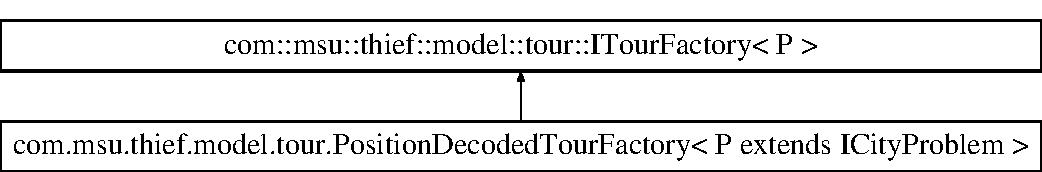
\includegraphics[height=2.000000cm]{classcom_1_1msu_1_1thief_1_1model_1_1tour_1_1PositionDecodedTourFactory_3_01P_01extends_01ICityProblem_01_4}
\end{center}
\end{figure}
\subsection*{Public Member Functions}
\begin{DoxyCompactItemize}
\item 
\hypertarget{classcom_1_1msu_1_1thief_1_1model_1_1tour_1_1PositionDecodedTourFactory_3_01P_01extends_01ICityProblem_01_4_aa7d01e1e51cc04d3cfec537264fb61bd}{Tour$<$?$>$ {\bfseries create} (P p)}\label{classcom_1_1msu_1_1thief_1_1model_1_1tour_1_1PositionDecodedTourFactory_3_01P_01extends_01ICityProblem_01_4_aa7d01e1e51cc04d3cfec537264fb61bd}

\end{DoxyCompactItemize}


\subsection{Detailed Description}
The \hyperlink{classcom_1_1msu_1_1thief_1_1model_1_1tour_1_1StandardTour}{Standard\-Tour} provides an implementation of a tour that saves directly the permutation array.

The encoding is nothing else than returning the array directly. 

The documentation for this class was generated from the following file\-:\begin{DoxyCompactItemize}
\item 
src/main/java/com/msu/thief/model/tour/Position\-Decoded\-Tour\-Factory.\-java\end{DoxyCompactItemize}

\hypertarget{classcom_1_1msu_1_1thief_1_1evaluator_1_1profit_1_1ProfitEvaluator}{\section{com.\-msu.\-thief.\-evaluator.\-profit.\-Profit\-Evaluator Class Reference}
\label{classcom_1_1msu_1_1thief_1_1evaluator_1_1profit_1_1ProfitEvaluator}\index{com.\-msu.\-thief.\-evaluator.\-profit.\-Profit\-Evaluator@{com.\-msu.\-thief.\-evaluator.\-profit.\-Profit\-Evaluator}}
}
Inheritance diagram for com.\-msu.\-thief.\-evaluator.\-profit.\-Profit\-Evaluator\-:\begin{figure}[H]
\begin{center}
\leavevmode
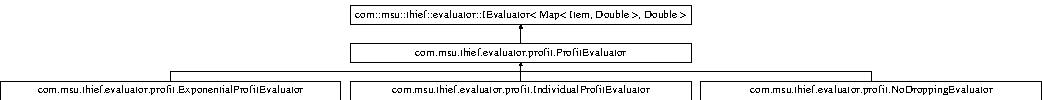
\includegraphics[height=1.346154cm]{classcom_1_1msu_1_1thief_1_1evaluator_1_1profit_1_1ProfitEvaluator}
\end{center}
\end{figure}


\subsection{Detailed Description}
The Profit\-Calculator provides an interface for calculating the profit. For each item the time how long it was inside of the knapsack has to be provided. 

The documentation for this class was generated from the following file\-:\begin{DoxyCompactItemize}
\item 
src/main/java/com/msu/thief/evaluator/profit/Profit\-Evaluator.\-java\end{DoxyCompactItemize}

\hypertarget{classcom_1_1msu_1_1thief_1_1experiment_1_1PublicationExperiment}{\section{com.\-msu.\-thief.\-experiment.\-Publication\-Experiment Class Reference}
\label{classcom_1_1msu_1_1thief_1_1experiment_1_1PublicationExperiment}\index{com.\-msu.\-thief.\-experiment.\-Publication\-Experiment@{com.\-msu.\-thief.\-experiment.\-Publication\-Experiment}}
}
Inheritance diagram for com.\-msu.\-thief.\-experiment.\-Publication\-Experiment\-:\begin{figure}[H]
\begin{center}
\leavevmode
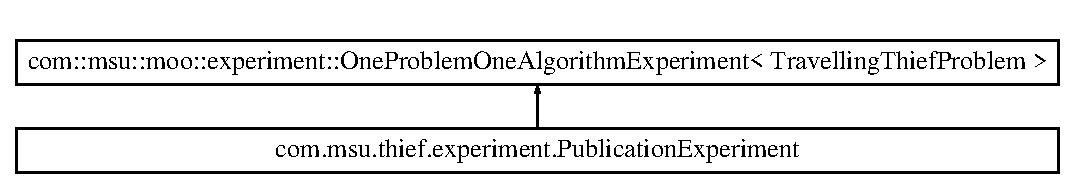
\includegraphics[height=2.000000cm]{classcom_1_1msu_1_1thief_1_1experiment_1_1PublicationExperiment}
\end{center}
\end{figure}
\subsection*{Public Member Functions}
\begin{DoxyCompactItemize}
\item 
\hypertarget{classcom_1_1msu_1_1thief_1_1experiment_1_1PublicationExperiment_aa7b381d93a130403ca2f27f581c74849}{void {\bfseries report} ()}\label{classcom_1_1msu_1_1thief_1_1experiment_1_1PublicationExperiment_aa7b381d93a130403ca2f27f581c74849}

\end{DoxyCompactItemize}
\subsection*{Protected Member Functions}
\begin{DoxyCompactItemize}
\item 
\hypertarget{classcom_1_1msu_1_1thief_1_1experiment_1_1PublicationExperiment_ada7b8e62d445bfbfab4e0079aed41602}{I\-Algorithm\\*
$<$ \hyperlink{classcom_1_1msu_1_1thief_1_1problems_1_1TravellingThiefProblem}{Travelling\-Thief\-Problem} $>$ {\bfseries get\-Algorithm} ()}\label{classcom_1_1msu_1_1thief_1_1experiment_1_1PublicationExperiment_ada7b8e62d445bfbfab4e0079aed41602}

\item 
\hypertarget{classcom_1_1msu_1_1thief_1_1experiment_1_1PublicationExperiment_af5db78e4e54fe3c728272442c3684ecf}{\hyperlink{classcom_1_1msu_1_1thief_1_1problems_1_1TravellingThiefProblem}{Travelling\-Thief\-Problem} {\bfseries get\-Problem} ()}\label{classcom_1_1msu_1_1thief_1_1experiment_1_1PublicationExperiment_af5db78e4e54fe3c728272442c3684ecf}

\item 
\hypertarget{classcom_1_1msu_1_1thief_1_1experiment_1_1PublicationExperiment_ab227139ff6e3056cd773ffbb3e582ac3}{Non\-Dominated\-Solution\-Set {\bfseries get\-True\-Front} ()}\label{classcom_1_1msu_1_1thief_1_1experiment_1_1PublicationExperiment_ab227139ff6e3056cd773ffbb3e582ac3}

\end{DoxyCompactItemize}


The documentation for this class was generated from the following file\-:\begin{DoxyCompactItemize}
\item 
src/main/java/com/msu/thief/experiment/Publication\-Experiment.\-java\end{DoxyCompactItemize}

\hypertarget{classcom_1_1msu_1_1thief_1_1evaluator_1_1time_1_1StandardTimeEvaluator}{\section{com.\-msu.\-thief.\-evaluator.\-time.\-Standard\-Time\-Evaluator Class Reference}
\label{classcom_1_1msu_1_1thief_1_1evaluator_1_1time_1_1StandardTimeEvaluator}\index{com.\-msu.\-thief.\-evaluator.\-time.\-Standard\-Time\-Evaluator@{com.\-msu.\-thief.\-evaluator.\-time.\-Standard\-Time\-Evaluator}}
}
Inheritance diagram for com.\-msu.\-thief.\-evaluator.\-time.\-Standard\-Time\-Evaluator\-:\begin{figure}[H]
\begin{center}
\leavevmode
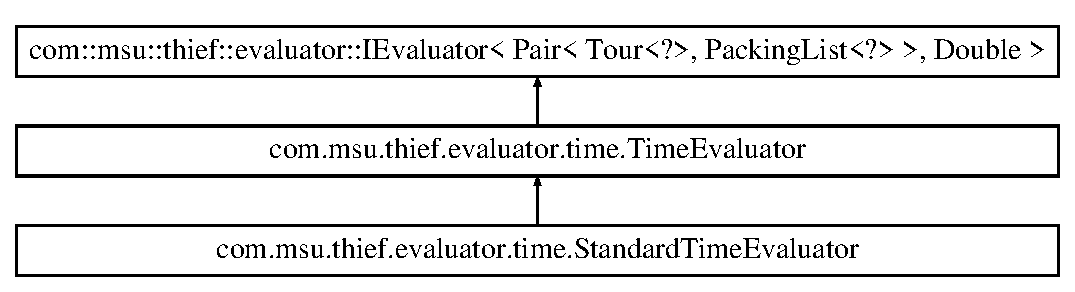
\includegraphics[height=3.000000cm]{classcom_1_1msu_1_1thief_1_1evaluator_1_1time_1_1StandardTimeEvaluator}
\end{center}
\end{figure}
\subsection*{Public Member Functions}
\begin{DoxyCompactItemize}
\item 
\hypertarget{classcom_1_1msu_1_1thief_1_1evaluator_1_1time_1_1StandardTimeEvaluator_ada2ccb007fd11c5e858b4227c0b3483f}{{\bfseries Standard\-Time\-Evaluator} (\hyperlink{classcom_1_1msu_1_1thief_1_1problems_1_1TravellingThiefProblem}{Travelling\-Thief\-Problem} problem)}\label{classcom_1_1msu_1_1thief_1_1evaluator_1_1time_1_1StandardTimeEvaluator_ada2ccb007fd11c5e858b4227c0b3483f}

\item 
\hypertarget{classcom_1_1msu_1_1thief_1_1evaluator_1_1time_1_1StandardTimeEvaluator_aeacf4ebaafa5b2327b7518bbb383a94f}{Double {\bfseries evaluate\-\_\-} (Pair$<$ Tour$<$?$>$, Packing\-List$<$?$>$$>$ input)}\label{classcom_1_1msu_1_1thief_1_1evaluator_1_1time_1_1StandardTimeEvaluator_aeacf4ebaafa5b2327b7518bbb383a94f}

\end{DoxyCompactItemize}
\subsection*{Additional Inherited Members}


The documentation for this class was generated from the following file\-:\begin{DoxyCompactItemize}
\item 
src/main/java/com/msu/thief/evaluator/time/Standard\-Time\-Evaluator.\-java\end{DoxyCompactItemize}

\hypertarget{classcom_1_1msu_1_1thief_1_1model_1_1tour_1_1StandardTour}{\section{com.\-msu.\-thief.\-model.\-tour.\-Standard\-Tour Class Reference}
\label{classcom_1_1msu_1_1thief_1_1model_1_1tour_1_1StandardTour}\index{com.\-msu.\-thief.\-model.\-tour.\-Standard\-Tour@{com.\-msu.\-thief.\-model.\-tour.\-Standard\-Tour}}
}
Inheritance diagram for com.\-msu.\-thief.\-model.\-tour.\-Standard\-Tour\-:\begin{figure}[H]
\begin{center}
\leavevmode
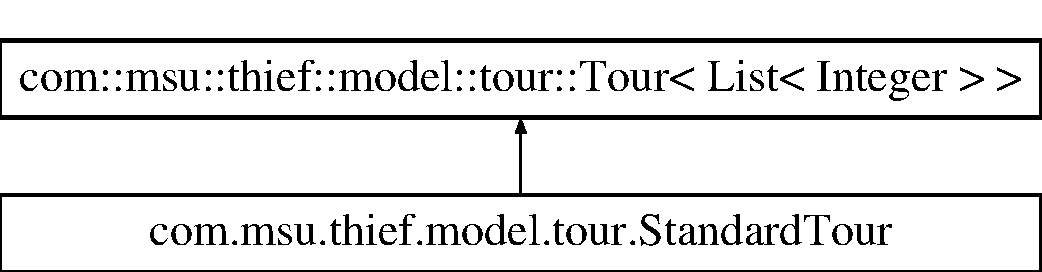
\includegraphics[height=2.000000cm]{classcom_1_1msu_1_1thief_1_1model_1_1tour_1_1StandardTour}
\end{center}
\end{figure}
\subsection*{Public Member Functions}
\begin{DoxyCompactItemize}
\item 
\hyperlink{classcom_1_1msu_1_1thief_1_1model_1_1tour_1_1StandardTour_a4098e8ce7d6c6067e7f83e8c558dc337}{Standard\-Tour} (List$<$ Integer $>$ list)
\item 
\hypertarget{classcom_1_1msu_1_1thief_1_1model_1_1tour_1_1StandardTour_aa31fa8362030accd4ee1a5fd04926b9e}{\hyperlink{classcom_1_1msu_1_1thief_1_1model_1_1tour_1_1StandardTour}{Standard\-Tour} {\bfseries copy} ()}\label{classcom_1_1msu_1_1thief_1_1model_1_1tour_1_1StandardTour_aa31fa8362030accd4ee1a5fd04926b9e}

\item 
\hypertarget{classcom_1_1msu_1_1thief_1_1model_1_1tour_1_1StandardTour_a3b08ec6d020b2e8ab7c3b00adf09f6ed}{List$<$ Integer $>$ {\bfseries encode} ()}\label{classcom_1_1msu_1_1thief_1_1model_1_1tour_1_1StandardTour_a3b08ec6d020b2e8ab7c3b00adf09f6ed}

\end{DoxyCompactItemize}


\subsection{Detailed Description}
The \hyperlink{classcom_1_1msu_1_1thief_1_1model_1_1tour_1_1StandardTour}{Standard\-Tour} provides an implementation of a tour that saves directly the permutation array.

The encoding is nothing else than returning the array directly. 

\subsection{Constructor \& Destructor Documentation}
\hypertarget{classcom_1_1msu_1_1thief_1_1model_1_1tour_1_1StandardTour_a4098e8ce7d6c6067e7f83e8c558dc337}{\index{com\-::msu\-::thief\-::model\-::tour\-::\-Standard\-Tour@{com\-::msu\-::thief\-::model\-::tour\-::\-Standard\-Tour}!Standard\-Tour@{Standard\-Tour}}
\index{Standard\-Tour@{Standard\-Tour}!com::msu::thief::model::tour::StandardTour@{com\-::msu\-::thief\-::model\-::tour\-::\-Standard\-Tour}}
\subsubsection[{Standard\-Tour}]{\setlength{\rightskip}{0pt plus 5cm}com.\-msu.\-thief.\-model.\-tour.\-Standard\-Tour.\-Standard\-Tour (
\begin{DoxyParamCaption}
\item[{List$<$ Integer $>$}]{list}
\end{DoxyParamCaption}
)\hspace{0.3cm}{\ttfamily [inline]}}}\label{classcom_1_1msu_1_1thief_1_1model_1_1tour_1_1StandardTour_a4098e8ce7d6c6067e7f83e8c558dc337}
Create a Tour using a permutation vector


\begin{DoxyParams}{Parameters}
{\em list} & tour represented by permutation vector \\
\hline
\end{DoxyParams}


The documentation for this class was generated from the following file\-:\begin{DoxyCompactItemize}
\item 
src/main/java/com/msu/thief/model/tour/Standard\-Tour.\-java\end{DoxyCompactItemize}

\hypertarget{classcom_1_1msu_1_1thief_1_1model_1_1tour_1_1StandardTourFactory_3_01P_01extends_01ICityProblem_01_4}{\section{com.\-msu.\-thief.\-model.\-tour.\-Standard\-Tour\-Factory$<$ P extends I\-City\-Problem $>$ Class Reference}
\label{classcom_1_1msu_1_1thief_1_1model_1_1tour_1_1StandardTourFactory_3_01P_01extends_01ICityProblem_01_4}\index{com.\-msu.\-thief.\-model.\-tour.\-Standard\-Tour\-Factory$<$ P extends I\-City\-Problem $>$@{com.\-msu.\-thief.\-model.\-tour.\-Standard\-Tour\-Factory$<$ P extends I\-City\-Problem $>$}}
}
Inheritance diagram for com.\-msu.\-thief.\-model.\-tour.\-Standard\-Tour\-Factory$<$ P extends I\-City\-Problem $>$\-:\begin{figure}[H]
\begin{center}
\leavevmode
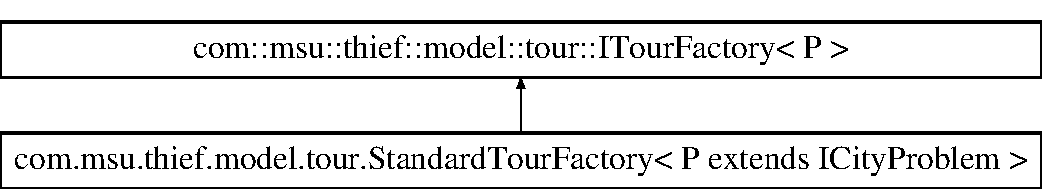
\includegraphics[height=2.000000cm]{classcom_1_1msu_1_1thief_1_1model_1_1tour_1_1StandardTourFactory_3_01P_01extends_01ICityProblem_01_4}
\end{center}
\end{figure}
\subsection*{Public Member Functions}
\begin{DoxyCompactItemize}
\item 
\hypertarget{classcom_1_1msu_1_1thief_1_1model_1_1tour_1_1StandardTourFactory_3_01P_01extends_01ICityProblem_01_4_a3fbbe36b85b38e3b73db96d3318793ba}{Tour$<$?$>$ {\bfseries create} (P p)}\label{classcom_1_1msu_1_1thief_1_1model_1_1tour_1_1StandardTourFactory_3_01P_01extends_01ICityProblem_01_4_a3fbbe36b85b38e3b73db96d3318793ba}

\end{DoxyCompactItemize}


The documentation for this class was generated from the following file\-:\begin{DoxyCompactItemize}
\item 
src/main/java/com/msu/thief/model/tour/Standard\-Tour\-Factory.\-java\end{DoxyCompactItemize}

\hypertarget{classcom_1_1msu_1_1thief_1_1model_1_1SymmetricMap}{\section{com.\-msu.\-thief.\-model.\-Symmetric\-Map Class Reference}
\label{classcom_1_1msu_1_1thief_1_1model_1_1SymmetricMap}\index{com.\-msu.\-thief.\-model.\-Symmetric\-Map@{com.\-msu.\-thief.\-model.\-Symmetric\-Map}}
}
\subsection*{Public Member Functions}
\begin{DoxyCompactItemize}
\item 
\hyperlink{classcom_1_1msu_1_1thief_1_1model_1_1SymmetricMap_a44db52139f57eef76ba9b64d61059af7}{Symmetric\-Map} (int n)
\item 
\hypertarget{classcom_1_1msu_1_1thief_1_1model_1_1SymmetricMap_ac58ed31c7760c1c8bfc7a158f85c7f4f}{double {\bfseries get} (int i, int j)}\label{classcom_1_1msu_1_1thief_1_1model_1_1SymmetricMap_ac58ed31c7760c1c8bfc7a158f85c7f4f}

\item 
\hypertarget{classcom_1_1msu_1_1thief_1_1model_1_1SymmetricMap_a75dc77beaa0bfee44a501d9f40aff019}{\hyperlink{classcom_1_1msu_1_1thief_1_1model_1_1SymmetricMap}{Symmetric\-Map} {\bfseries set} (int i, int j, double value)}\label{classcom_1_1msu_1_1thief_1_1model_1_1SymmetricMap_a75dc77beaa0bfee44a501d9f40aff019}

\item 
\hypertarget{classcom_1_1msu_1_1thief_1_1model_1_1SymmetricMap_a13d6b4f187e2ae9f1e41d33f226b461c}{int {\bfseries get\-Size} ()}\label{classcom_1_1msu_1_1thief_1_1model_1_1SymmetricMap_a13d6b4f187e2ae9f1e41d33f226b461c}

\item 
\hypertarget{classcom_1_1msu_1_1thief_1_1model_1_1SymmetricMap_a729ec92b46e9a023477064db6d20d3e4}{double {\bfseries get\-Min} ()}\label{classcom_1_1msu_1_1thief_1_1model_1_1SymmetricMap_a729ec92b46e9a023477064db6d20d3e4}

\item 
\hypertarget{classcom_1_1msu_1_1thief_1_1model_1_1SymmetricMap_a1018195e0b1876d71b35254921b00ea5}{double {\bfseries get\-Max} ()}\label{classcom_1_1msu_1_1thief_1_1model_1_1SymmetricMap_a1018195e0b1876d71b35254921b00ea5}

\item 
void \hyperlink{classcom_1_1msu_1_1thief_1_1model_1_1SymmetricMap_ac3d0ed542debc70ee277486a9dddcb08}{set\-Distances} (double\mbox{[}$\,$\mbox{]}\mbox{[}$\,$\mbox{]} \hyperlink{classcom_1_1msu_1_1thief_1_1model_1_1SymmetricMap_a9807f5fdaef9e484d40fe13dfe7abc0d}{distances})
\end{DoxyCompactItemize}
\subsection*{Protected Attributes}
\begin{DoxyCompactItemize}
\item 
\hypertarget{classcom_1_1msu_1_1thief_1_1model_1_1SymmetricMap_a9807f5fdaef9e484d40fe13dfe7abc0d}{double\mbox{[}$\,$\mbox{]}\mbox{[}$\,$\mbox{]} \hyperlink{classcom_1_1msu_1_1thief_1_1model_1_1SymmetricMap_a9807f5fdaef9e484d40fe13dfe7abc0d}{distances}}\label{classcom_1_1msu_1_1thief_1_1model_1_1SymmetricMap_a9807f5fdaef9e484d40fe13dfe7abc0d}

\begin{DoxyCompactList}\small\item\em distance matrix \end{DoxyCompactList}\item 
\hypertarget{classcom_1_1msu_1_1thief_1_1model_1_1SymmetricMap_a0a8541e5a74bf2c3dbfa289fe7a91c3f}{double \hyperlink{classcom_1_1msu_1_1thief_1_1model_1_1SymmetricMap_a0a8541e5a74bf2c3dbfa289fe7a91c3f}{min} = Double.\-M\-A\-X\-\_\-\-V\-A\-L\-U\-E}\label{classcom_1_1msu_1_1thief_1_1model_1_1SymmetricMap_a0a8541e5a74bf2c3dbfa289fe7a91c3f}

\begin{DoxyCompactList}\small\item\em minimal distance \end{DoxyCompactList}\item 
\hypertarget{classcom_1_1msu_1_1thief_1_1model_1_1SymmetricMap_a688182c87e1c31cb09a004532eb699b9}{double \hyperlink{classcom_1_1msu_1_1thief_1_1model_1_1SymmetricMap_a688182c87e1c31cb09a004532eb699b9}{max} = Double.\-M\-I\-N\-\_\-\-V\-A\-L\-U\-E}\label{classcom_1_1msu_1_1thief_1_1model_1_1SymmetricMap_a688182c87e1c31cb09a004532eb699b9}

\begin{DoxyCompactList}\small\item\em maximal distance \end{DoxyCompactList}\end{DoxyCompactItemize}


\subsection{Detailed Description}
This class represents a map with a predefined number of cities. It is a symmetrical map where where the \mbox{[}i\mbox{]}\mbox{[}j\mbox{]} value will always be the same as the \mbox{[}j\mbox{]}\mbox{[}i\mbox{]} value.

Also the class provides to get the minimal and the maximal distance all the time! 

\subsection{Constructor \& Destructor Documentation}
\hypertarget{classcom_1_1msu_1_1thief_1_1model_1_1SymmetricMap_a44db52139f57eef76ba9b64d61059af7}{\index{com\-::msu\-::thief\-::model\-::\-Symmetric\-Map@{com\-::msu\-::thief\-::model\-::\-Symmetric\-Map}!Symmetric\-Map@{Symmetric\-Map}}
\index{Symmetric\-Map@{Symmetric\-Map}!com::msu::thief::model::SymmetricMap@{com\-::msu\-::thief\-::model\-::\-Symmetric\-Map}}
\subsubsection[{Symmetric\-Map}]{\setlength{\rightskip}{0pt plus 5cm}com.\-msu.\-thief.\-model.\-Symmetric\-Map.\-Symmetric\-Map (
\begin{DoxyParamCaption}
\item[{int}]{n}
\end{DoxyParamCaption}
)\hspace{0.3cm}{\ttfamily [inline]}}}\label{classcom_1_1msu_1_1thief_1_1model_1_1SymmetricMap_a44db52139f57eef76ba9b64d61059af7}
Construct where all distance are zero. 
\begin{DoxyParams}{Parameters}
{\em n} & \\
\hline
\end{DoxyParams}


\subsection{Member Function Documentation}
\hypertarget{classcom_1_1msu_1_1thief_1_1model_1_1SymmetricMap_ac3d0ed542debc70ee277486a9dddcb08}{\index{com\-::msu\-::thief\-::model\-::\-Symmetric\-Map@{com\-::msu\-::thief\-::model\-::\-Symmetric\-Map}!set\-Distances@{set\-Distances}}
\index{set\-Distances@{set\-Distances}!com::msu::thief::model::SymmetricMap@{com\-::msu\-::thief\-::model\-::\-Symmetric\-Map}}
\subsubsection[{set\-Distances}]{\setlength{\rightskip}{0pt plus 5cm}void com.\-msu.\-thief.\-model.\-Symmetric\-Map.\-set\-Distances (
\begin{DoxyParamCaption}
\item[{double}]{distances\mbox{[}$\,$\mbox{]}\mbox{[}$\,$\mbox{]}}
\end{DoxyParamCaption}
)\hspace{0.3cm}{\ttfamily [inline]}}}\label{classcom_1_1msu_1_1thief_1_1model_1_1SymmetricMap_ac3d0ed542debc70ee277486a9dddcb08}
Be careful when using this method. It trusts the user! 
\begin{DoxyParams}{Parameters}
{\em distances} & cost matrix \\
\hline
\end{DoxyParams}


The documentation for this class was generated from the following file\-:\begin{DoxyCompactItemize}
\item 
src/main/java/com/msu/thief/model/Symmetric\-Map.\-java\end{DoxyCompactItemize}

\hypertarget{classcom_1_1msu_1_1thief_1_1factory_1_1ThiefProblemFactory}{\section{com.\-msu.\-thief.\-factory.\-Thief\-Problem\-Factory Class Reference}
\label{classcom_1_1msu_1_1thief_1_1factory_1_1ThiefProblemFactory}\index{com.\-msu.\-thief.\-factory.\-Thief\-Problem\-Factory@{com.\-msu.\-thief.\-factory.\-Thief\-Problem\-Factory}}
}
\subsection*{Classes}
\begin{DoxyCompactItemize}
\item 
enum {\bfseries D\-R\-O\-P\-P\-I\-N\-G\-\_\-\-T\-Y\-P\-E}
\end{DoxyCompactItemize}
\subsection*{Public Member Functions}
\begin{DoxyCompactItemize}
\item 
\hypertarget{classcom_1_1msu_1_1thief_1_1factory_1_1ThiefProblemFactory_a8aefd104d204b50b7d28f76e4b298b99}{{\bfseries Thief\-Problem\-Factory} (\hyperlink{classcom_1_1msu_1_1thief_1_1factory_1_1map_1_1MapFactory}{Map\-Factory} fac\-Map, \hyperlink{classcom_1_1msu_1_1thief_1_1factory_1_1items_1_1ItemFactory}{Item\-Factory} fac\-Items, Double max\-Weight\-Perc)}\label{classcom_1_1msu_1_1thief_1_1factory_1_1ThiefProblemFactory_a8aefd104d204b50b7d28f76e4b298b99}

\item 
\hypertarget{classcom_1_1msu_1_1thief_1_1factory_1_1ThiefProblemFactory_acb89875dc4e53818403d1c2d75f52724}{{\bfseries Thief\-Problem\-Factory} (\hyperlink{classcom_1_1msu_1_1thief_1_1factory_1_1map_1_1MapFactory}{Map\-Factory} fac\-Map, \hyperlink{classcom_1_1msu_1_1thief_1_1factory_1_1items_1_1ItemFactory}{Item\-Factory} fac\-Items, Double max\-Weight\-Perc, String name)}\label{classcom_1_1msu_1_1thief_1_1factory_1_1ThiefProblemFactory_acb89875dc4e53818403d1c2d75f52724}

\item 
\hypertarget{classcom_1_1msu_1_1thief_1_1factory_1_1ThiefProblemFactory_ab1973fba70b16cba2e3bde7487348f30}{\hyperlink{classcom_1_1msu_1_1thief_1_1problems_1_1TravellingThiefProblem}{Travelling\-Thief\-Problem} {\bfseries create} (int num\-Of\-Cities, int items\-Per\-City)}\label{classcom_1_1msu_1_1thief_1_1factory_1_1ThiefProblemFactory_ab1973fba70b16cba2e3bde7487348f30}

\item 
\hypertarget{classcom_1_1msu_1_1thief_1_1factory_1_1ThiefProblemFactory_ad0d5e76dda951d5afc7c65ecf0144715}{D\-R\-O\-P\-P\-I\-N\-G\-\_\-\-T\-Y\-P\-E {\bfseries get\-Drop\-Type} ()}\label{classcom_1_1msu_1_1thief_1_1factory_1_1ThiefProblemFactory_ad0d5e76dda951d5afc7c65ecf0144715}

\item 
\hypertarget{classcom_1_1msu_1_1thief_1_1factory_1_1ThiefProblemFactory_ac2117b063c88fb607d2d112c4a129465}{void {\bfseries set\-Drop\-Type} (D\-R\-O\-P\-P\-I\-N\-G\-\_\-\-T\-Y\-P\-E drop\-Type)}\label{classcom_1_1msu_1_1thief_1_1factory_1_1ThiefProblemFactory_ac2117b063c88fb607d2d112c4a129465}

\item 
\hypertarget{classcom_1_1msu_1_1thief_1_1factory_1_1ThiefProblemFactory_aa700094ef4d896d26854cdacb858ef77}{\hyperlink{classcom_1_1msu_1_1thief_1_1factory_1_1map_1_1MapFactory}{Map\-Factory} {\bfseries get\-Fac\-Map} ()}\label{classcom_1_1msu_1_1thief_1_1factory_1_1ThiefProblemFactory_aa700094ef4d896d26854cdacb858ef77}

\item 
\hypertarget{classcom_1_1msu_1_1thief_1_1factory_1_1ThiefProblemFactory_ade589bec00fdb94fb77334e77e248166}{void {\bfseries set\-Fac\-Map} (\hyperlink{classcom_1_1msu_1_1thief_1_1factory_1_1map_1_1MapFactory}{Map\-Factory} fac\-Map)}\label{classcom_1_1msu_1_1thief_1_1factory_1_1ThiefProblemFactory_ade589bec00fdb94fb77334e77e248166}

\item 
\hypertarget{classcom_1_1msu_1_1thief_1_1factory_1_1ThiefProblemFactory_a6a430a34d8b5fe7bc3d208336feccd4d}{\hyperlink{classcom_1_1msu_1_1thief_1_1factory_1_1items_1_1ItemFactory}{Item\-Factory} {\bfseries get\-Fac\-Items} ()}\label{classcom_1_1msu_1_1thief_1_1factory_1_1ThiefProblemFactory_a6a430a34d8b5fe7bc3d208336feccd4d}

\item 
\hypertarget{classcom_1_1msu_1_1thief_1_1factory_1_1ThiefProblemFactory_ab0a7d9c6f2f5872f36ff666b6d4b0531}{void {\bfseries set\-Fac\-Items} (\hyperlink{classcom_1_1msu_1_1thief_1_1factory_1_1items_1_1ItemFactory}{Item\-Factory} fac\-Items)}\label{classcom_1_1msu_1_1thief_1_1factory_1_1ThiefProblemFactory_ab0a7d9c6f2f5872f36ff666b6d4b0531}

\item 
\hypertarget{classcom_1_1msu_1_1thief_1_1factory_1_1ThiefProblemFactory_a5c74bdc58ffdd4aa8cc5101cd5f187d8}{Double {\bfseries get\-Max\-Weight\-Perc} ()}\label{classcom_1_1msu_1_1thief_1_1factory_1_1ThiefProblemFactory_a5c74bdc58ffdd4aa8cc5101cd5f187d8}

\item 
\hypertarget{classcom_1_1msu_1_1thief_1_1factory_1_1ThiefProblemFactory_a5d4ebae3817de208bf145fb0e5593451}{void {\bfseries set\-Max\-Weight\-Perc} (Double max\-Weight\-Perc)}\label{classcom_1_1msu_1_1thief_1_1factory_1_1ThiefProblemFactory_a5d4ebae3817de208bf145fb0e5593451}

\item 
\hypertarget{classcom_1_1msu_1_1thief_1_1factory_1_1ThiefProblemFactory_abaf4591774292f1dd58a413c09178f09}{String {\bfseries get\-Name} ()}\label{classcom_1_1msu_1_1thief_1_1factory_1_1ThiefProblemFactory_abaf4591774292f1dd58a413c09178f09}

\item 
\hypertarget{classcom_1_1msu_1_1thief_1_1factory_1_1ThiefProblemFactory_a25bb46403ae388ffcb64b8b82d0f2716}{void {\bfseries set\-Name} (String name)}\label{classcom_1_1msu_1_1thief_1_1factory_1_1ThiefProblemFactory_a25bb46403ae388ffcb64b8b82d0f2716}

\end{DoxyCompactItemize}
\subsection*{Protected Attributes}
\begin{DoxyCompactItemize}
\item 
\hypertarget{classcom_1_1msu_1_1thief_1_1factory_1_1ThiefProblemFactory_a4d7c11f2f45909bf17ec9be46d73f8e0}{D\-R\-O\-P\-P\-I\-N\-G\-\_\-\-T\-Y\-P\-E {\bfseries drop\-Type} = D\-R\-O\-P\-P\-I\-N\-G\-\_\-\-T\-Y\-P\-E.\-M\-A\-X\-\_\-\-D\-I\-S\-T\-A\-N\-C\-E\-\_\-\-D\-E\-P\-E\-N\-D\-E\-N\-T}\label{classcom_1_1msu_1_1thief_1_1factory_1_1ThiefProblemFactory_a4d7c11f2f45909bf17ec9be46d73f8e0}

\item 
\hypertarget{classcom_1_1msu_1_1thief_1_1factory_1_1ThiefProblemFactory_a58fdea42e46e2b553ac1ca1c05feb6e9}{\hyperlink{classcom_1_1msu_1_1thief_1_1factory_1_1map_1_1MapFactory}{Map\-Factory} {\bfseries fac\-Map} = null}\label{classcom_1_1msu_1_1thief_1_1factory_1_1ThiefProblemFactory_a58fdea42e46e2b553ac1ca1c05feb6e9}

\item 
\hypertarget{classcom_1_1msu_1_1thief_1_1factory_1_1ThiefProblemFactory_a8c0d90d270932e8a2f0a34985b3b296c}{\hyperlink{classcom_1_1msu_1_1thief_1_1factory_1_1items_1_1ItemFactory}{Item\-Factory} {\bfseries fac\-Items} = null}\label{classcom_1_1msu_1_1thief_1_1factory_1_1ThiefProblemFactory_a8c0d90d270932e8a2f0a34985b3b296c}

\item 
\hypertarget{classcom_1_1msu_1_1thief_1_1factory_1_1ThiefProblemFactory_a082b34613fedf0177a74c03890528c60}{Double {\bfseries max\-Weight\-Perc} = null}\label{classcom_1_1msu_1_1thief_1_1factory_1_1ThiefProblemFactory_a082b34613fedf0177a74c03890528c60}

\item 
\hypertarget{classcom_1_1msu_1_1thief_1_1factory_1_1ThiefProblemFactory_a9803d3e81e6954b576727b7c8e8870f2}{String {\bfseries name} = null}\label{classcom_1_1msu_1_1thief_1_1factory_1_1ThiefProblemFactory_a9803d3e81e6954b576727b7c8e8870f2}

\end{DoxyCompactItemize}


\subsection{Detailed Description}
This class represents a thief factory which allows to create a Travelling\-Thief Problem. 

The documentation for this class was generated from the following file\-:\begin{DoxyCompactItemize}
\item 
src/main/java/com/msu/thief/factory/Thief\-Problem\-Factory.\-java\end{DoxyCompactItemize}

\hypertarget{classcom_1_1msu_1_1thief_1_1evaluator_1_1time_1_1TimeEvaluator}{\section{com.\-msu.\-thief.\-evaluator.\-time.\-Time\-Evaluator Class Reference}
\label{classcom_1_1msu_1_1thief_1_1evaluator_1_1time_1_1TimeEvaluator}\index{com.\-msu.\-thief.\-evaluator.\-time.\-Time\-Evaluator@{com.\-msu.\-thief.\-evaluator.\-time.\-Time\-Evaluator}}
}
Inheritance diagram for com.\-msu.\-thief.\-evaluator.\-time.\-Time\-Evaluator\-:\begin{figure}[H]
\begin{center}
\leavevmode
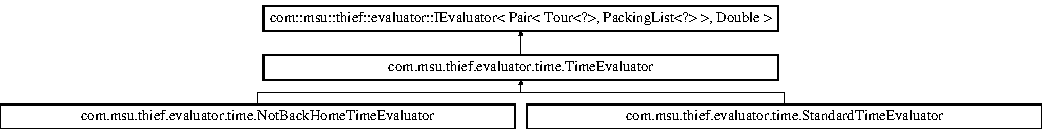
\includegraphics[height=1.735537cm]{classcom_1_1msu_1_1thief_1_1evaluator_1_1time_1_1TimeEvaluator}
\end{center}
\end{figure}
\subsection*{Public Member Functions}
\begin{DoxyCompactItemize}
\item 
\hypertarget{classcom_1_1msu_1_1thief_1_1evaluator_1_1time_1_1TimeEvaluator_aec5919eb1094217c4c15f203ddffb0c7}{{\bfseries Time\-Evaluator} (\hyperlink{classcom_1_1msu_1_1thief_1_1problems_1_1TravellingThiefProblem}{Travelling\-Thief\-Problem} problem)}\label{classcom_1_1msu_1_1thief_1_1evaluator_1_1time_1_1TimeEvaluator_aec5919eb1094217c4c15f203ddffb0c7}

\item 
\hypertarget{classcom_1_1msu_1_1thief_1_1evaluator_1_1time_1_1TimeEvaluator_a39a77d5389465bac3be3daa2d58ceedf}{Double {\bfseries get\-Weight} ()}\label{classcom_1_1msu_1_1thief_1_1evaluator_1_1time_1_1TimeEvaluator_a39a77d5389465bac3be3daa2d58ceedf}

\item 
\hypertarget{classcom_1_1msu_1_1thief_1_1evaluator_1_1time_1_1TimeEvaluator_ade92825af0ef8792561b7ab2971870a3}{Double {\bfseries get\-Time} ()}\label{classcom_1_1msu_1_1thief_1_1evaluator_1_1time_1_1TimeEvaluator_ade92825af0ef8792561b7ab2971870a3}

\item 
\hypertarget{classcom_1_1msu_1_1thief_1_1evaluator_1_1time_1_1TimeEvaluator_ace791e85c5b203add7bcd874eceda9cd}{Map$<$ \hyperlink{classcom_1_1msu_1_1thief_1_1model_1_1Item}{Item}, Double $>$ {\bfseries get\-Item\-Map} ()}\label{classcom_1_1msu_1_1thief_1_1evaluator_1_1time_1_1TimeEvaluator_ace791e85c5b203add7bcd874eceda9cd}

\item 
\hypertarget{classcom_1_1msu_1_1thief_1_1evaluator_1_1time_1_1TimeEvaluator_a6fce957d73ab6ae5cca29c920cd5aafc}{Double {\bfseries evaluate} (Pair$<$ Tour$<$?$>$, Packing\-List$<$?$>$$>$ input)}\label{classcom_1_1msu_1_1thief_1_1evaluator_1_1time_1_1TimeEvaluator_a6fce957d73ab6ae5cca29c920cd5aafc}

\item 
\hypertarget{classcom_1_1msu_1_1thief_1_1evaluator_1_1time_1_1TimeEvaluator_a26328a49fde69f2b4a3419ac74dc5c30}{abstract Double {\bfseries evaluate\-\_\-} (Pair$<$ Tour$<$?$>$, Packing\-List$<$?$>$$>$ input)}\label{classcom_1_1msu_1_1thief_1_1evaluator_1_1time_1_1TimeEvaluator_a26328a49fde69f2b4a3419ac74dc5c30}

\end{DoxyCompactItemize}
\subsection*{Protected Attributes}
\begin{DoxyCompactItemize}
\item 
\hypertarget{classcom_1_1msu_1_1thief_1_1evaluator_1_1time_1_1TimeEvaluator_a47bbfd6b153b0b4baf5d5378cd41ed61}{\hyperlink{classcom_1_1msu_1_1thief_1_1problems_1_1TravellingThiefProblem}{Travelling\-Thief\-Problem} {\bfseries problem}}\label{classcom_1_1msu_1_1thief_1_1evaluator_1_1time_1_1TimeEvaluator_a47bbfd6b153b0b4baf5d5378cd41ed61}

\item 
\hypertarget{classcom_1_1msu_1_1thief_1_1evaluator_1_1time_1_1TimeEvaluator_ab9023ee339852c4736395dc9cd8fe219}{Double \hyperlink{classcom_1_1msu_1_1thief_1_1evaluator_1_1time_1_1TimeEvaluator_ab9023ee339852c4736395dc9cd8fe219}{time} = null}\label{classcom_1_1msu_1_1thief_1_1evaluator_1_1time_1_1TimeEvaluator_ab9023ee339852c4736395dc9cd8fe219}

\begin{DoxyCompactList}\small\item\em traveling time of the salesman \end{DoxyCompactList}\item 
\hypertarget{classcom_1_1msu_1_1thief_1_1evaluator_1_1time_1_1TimeEvaluator_a440dd0dfafd4d1bb162987966680677e}{Double \hyperlink{classcom_1_1msu_1_1thief_1_1evaluator_1_1time_1_1TimeEvaluator_a440dd0dfafd4d1bb162987966680677e}{weight} = null}\label{classcom_1_1msu_1_1thief_1_1evaluator_1_1time_1_1TimeEvaluator_a440dd0dfafd4d1bb162987966680677e}

\begin{DoxyCompactList}\small\item\em final weight of the knapsack \end{DoxyCompactList}\item 
\hypertarget{classcom_1_1msu_1_1thief_1_1evaluator_1_1time_1_1TimeEvaluator_a9db8192f4769aaa538cccc41d230bc27}{Map$<$ \hyperlink{classcom_1_1msu_1_1thief_1_1model_1_1Item}{Item}, Double $>$ \hyperlink{classcom_1_1msu_1_1thief_1_1evaluator_1_1time_1_1TimeEvaluator_a9db8192f4769aaa538cccc41d230bc27}{m\-Item} = new Hash\-Map$<$$>$()}\label{classcom_1_1msu_1_1thief_1_1evaluator_1_1time_1_1TimeEvaluator_a9db8192f4769aaa538cccc41d230bc27}

\begin{DoxyCompactList}\small\item\em mapping of the items and the packing duration \end{DoxyCompactList}\end{DoxyCompactItemize}


\subsection{Detailed Description}
The Time\-Calculator provides an interface for calculating the time of a given tour. 

The documentation for this class was generated from the following file\-:\begin{DoxyCompactItemize}
\item 
src/main/java/com/msu/thief/evaluator/time/Time\-Evaluator.\-java\end{DoxyCompactItemize}

\hypertarget{classcom_1_1msu_1_1thief_1_1model_1_1tour_1_1Tour_3_01T_01_4}{\section{com.\-msu.\-thief.\-model.\-tour.\-Tour$<$ T $>$ Class Reference}
\label{classcom_1_1msu_1_1thief_1_1model_1_1tour_1_1Tour_3_01T_01_4}\index{com.\-msu.\-thief.\-model.\-tour.\-Tour$<$ T $>$@{com.\-msu.\-thief.\-model.\-tour.\-Tour$<$ T $>$}}
}
Inheritance diagram for com.\-msu.\-thief.\-model.\-tour.\-Tour$<$ T $>$\-:\begin{figure}[H]
\begin{center}
\leavevmode
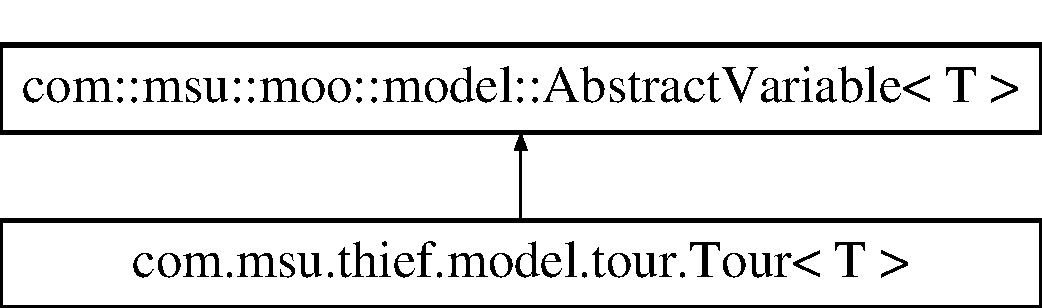
\includegraphics[height=2.000000cm]{classcom_1_1msu_1_1thief_1_1model_1_1tour_1_1Tour_3_01T_01_4}
\end{center}
\end{figure}
\subsection*{Public Member Functions}
\begin{DoxyCompactItemize}
\item 
\hypertarget{classcom_1_1msu_1_1thief_1_1model_1_1tour_1_1Tour_3_01T_01_4_a5d6f18d12c1ed867e4433c4f89ac0063}{{\bfseries Tour} (T obj)}\label{classcom_1_1msu_1_1thief_1_1model_1_1tour_1_1Tour_3_01T_01_4_a5d6f18d12c1ed867e4433c4f89ac0063}

\item 
\hypertarget{classcom_1_1msu_1_1thief_1_1model_1_1tour_1_1Tour_3_01T_01_4_a078a8d0928325d814d428dcd3b71e3a7}{String {\bfseries to\-String} ()}\label{classcom_1_1msu_1_1thief_1_1model_1_1tour_1_1Tour_3_01T_01_4_a078a8d0928325d814d428dcd3b71e3a7}

\item 
\hypertarget{classcom_1_1msu_1_1thief_1_1model_1_1tour_1_1Tour_3_01T_01_4_a85f94456f78ae727eaaa64f921bb0c07}{abstract List$<$ Integer $>$ {\bfseries encode} ()}\label{classcom_1_1msu_1_1thief_1_1model_1_1tour_1_1Tour_3_01T_01_4_a85f94456f78ae727eaaa64f921bb0c07}

\end{DoxyCompactItemize}


\subsection{Detailed Description}
This class represents the interface of a tour. Since there are different representation of tours which could be all encoded to the permutation representation. 

The documentation for this class was generated from the following file\-:\begin{DoxyCompactItemize}
\item 
src/main/java/com/msu/thief/model/tour/Tour.\-java\end{DoxyCompactItemize}

\hypertarget{classcom_1_1msu_1_1tsp_1_1TravellingSalesmanProblem}{\section{com.\-msu.\-tsp.\-Travelling\-Salesman\-Problem Class Reference}
\label{classcom_1_1msu_1_1tsp_1_1TravellingSalesmanProblem}\index{com.\-msu.\-tsp.\-Travelling\-Salesman\-Problem@{com.\-msu.\-tsp.\-Travelling\-Salesman\-Problem}}
}
Inheritance diagram for com.\-msu.\-tsp.\-Travelling\-Salesman\-Problem\-:\begin{figure}[H]
\begin{center}
\leavevmode
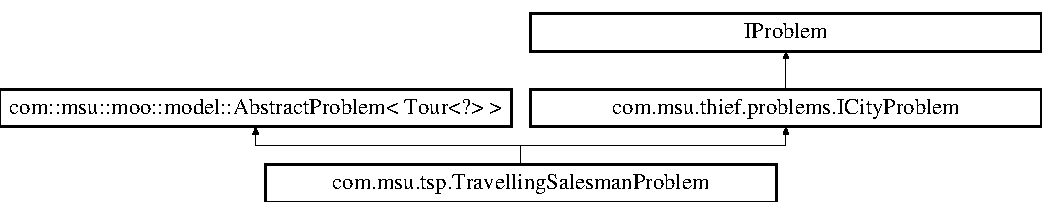
\includegraphics[height=2.718446cm]{classcom_1_1msu_1_1tsp_1_1TravellingSalesmanProblem}
\end{center}
\end{figure}
\subsection*{Public Member Functions}
\begin{DoxyCompactItemize}
\item 
\hyperlink{classcom_1_1msu_1_1tsp_1_1TravellingSalesmanProblem_a0a5878269d3ef19bcae96cefd7780203}{Travelling\-Salesman\-Problem} (\hyperlink{classcom_1_1msu_1_1thief_1_1model_1_1SymmetricMap}{Symmetric\-Map} map)
\item 
Double \hyperlink{classcom_1_1msu_1_1tsp_1_1TravellingSalesmanProblem_a798e3f5291752f96cdad115704e18d7a}{evaluate} (List$<$ Integer $>$ pi)
\item 
\hypertarget{classcom_1_1msu_1_1tsp_1_1TravellingSalesmanProblem_a579ec22ec3327c72aaf05e2b4649af3f}{int {\bfseries get\-Number\-Of\-Objectives} ()}\label{classcom_1_1msu_1_1tsp_1_1TravellingSalesmanProblem_a579ec22ec3327c72aaf05e2b4649af3f}

\item 
\hypertarget{classcom_1_1msu_1_1tsp_1_1TravellingSalesmanProblem_a07ba09f7b9170509441f9d2926158f51}{int {\bfseries num\-Of\-Cities} ()}\label{classcom_1_1msu_1_1tsp_1_1TravellingSalesmanProblem_a07ba09f7b9170509441f9d2926158f51}

\item 
\hypertarget{classcom_1_1msu_1_1tsp_1_1TravellingSalesmanProblem_a10b90d40349c85a3f648158e9fa5a523}{\hyperlink{classcom_1_1msu_1_1thief_1_1model_1_1SymmetricMap}{Symmetric\-Map} {\bfseries get\-Map} ()}\label{classcom_1_1msu_1_1tsp_1_1TravellingSalesmanProblem_a10b90d40349c85a3f648158e9fa5a523}

\end{DoxyCompactItemize}
\subsection*{Static Public Member Functions}
\begin{DoxyCompactItemize}
\item 
static void \hyperlink{classcom_1_1msu_1_1tsp_1_1TravellingSalesmanProblem_ad95a98935d07fa7acd8cb505d00c7d2f}{check\-Tour\-Size} (int size, List$<$ Integer $>$ pi)
\item 
static void \hyperlink{classcom_1_1msu_1_1tsp_1_1TravellingSalesmanProblem_ab1efe77a150e9413156162105ae954bf}{check\-Tour\-Validtiy} (List$<$ Integer $>$ pi)
\end{DoxyCompactItemize}
\subsection*{Protected Member Functions}
\begin{DoxyCompactItemize}
\item 
\hypertarget{classcom_1_1msu_1_1tsp_1_1TravellingSalesmanProblem_ac9587ac7ae89eaf8ff668a1b5ffa0ee6}{List$<$ Double $>$ {\bfseries evaluate\-\_\-} (Tour$<$?$>$ variable)}\label{classcom_1_1msu_1_1tsp_1_1TravellingSalesmanProblem_ac9587ac7ae89eaf8ff668a1b5ffa0ee6}

\end{DoxyCompactItemize}
\subsection*{Protected Attributes}
\begin{DoxyCompactItemize}
\item 
\hypertarget{classcom_1_1msu_1_1tsp_1_1TravellingSalesmanProblem_adf1dcf831a6523d1eb26ef2cdcb759e4}{\hyperlink{classcom_1_1msu_1_1thief_1_1model_1_1SymmetricMap}{Symmetric\-Map} {\bfseries map}}\label{classcom_1_1msu_1_1tsp_1_1TravellingSalesmanProblem_adf1dcf831a6523d1eb26ef2cdcb759e4}

\end{DoxyCompactItemize}


\subsection{Detailed Description}
This class defines the \hyperlink{classcom_1_1msu_1_1tsp_1_1TravellingSalesmanProblem}{Travelling\-Salesman\-Problem} which aims to minimize the tour distance of a salesman on a given map. 

\subsection{Constructor \& Destructor Documentation}
\hypertarget{classcom_1_1msu_1_1tsp_1_1TravellingSalesmanProblem_a0a5878269d3ef19bcae96cefd7780203}{\index{com\-::msu\-::tsp\-::\-Travelling\-Salesman\-Problem@{com\-::msu\-::tsp\-::\-Travelling\-Salesman\-Problem}!Travelling\-Salesman\-Problem@{Travelling\-Salesman\-Problem}}
\index{Travelling\-Salesman\-Problem@{Travelling\-Salesman\-Problem}!com::msu::tsp::TravellingSalesmanProblem@{com\-::msu\-::tsp\-::\-Travelling\-Salesman\-Problem}}
\subsubsection[{Travelling\-Salesman\-Problem}]{\setlength{\rightskip}{0pt plus 5cm}com.\-msu.\-tsp.\-Travelling\-Salesman\-Problem.\-Travelling\-Salesman\-Problem (
\begin{DoxyParamCaption}
\item[{{\bf Symmetric\-Map}}]{map}
\end{DoxyParamCaption}
)\hspace{0.3cm}{\ttfamily [inline]}}}\label{classcom_1_1msu_1_1tsp_1_1TravellingSalesmanProblem_a0a5878269d3ef19bcae96cefd7780203}
Construct a \hyperlink{classcom_1_1msu_1_1tsp_1_1TravellingSalesmanProblem}{Travelling\-Salesman\-Problem} by using a predefined map which provides a distance matrix.


\begin{DoxyParams}{Parameters}
{\em map} & object which defines the distances \\
\hline
\end{DoxyParams}


\subsection{Member Function Documentation}
\hypertarget{classcom_1_1msu_1_1tsp_1_1TravellingSalesmanProblem_ad95a98935d07fa7acd8cb505d00c7d2f}{\index{com\-::msu\-::tsp\-::\-Travelling\-Salesman\-Problem@{com\-::msu\-::tsp\-::\-Travelling\-Salesman\-Problem}!check\-Tour\-Size@{check\-Tour\-Size}}
\index{check\-Tour\-Size@{check\-Tour\-Size}!com::msu::tsp::TravellingSalesmanProblem@{com\-::msu\-::tsp\-::\-Travelling\-Salesman\-Problem}}
\subsubsection[{check\-Tour\-Size}]{\setlength{\rightskip}{0pt plus 5cm}static void com.\-msu.\-tsp.\-Travelling\-Salesman\-Problem.\-check\-Tour\-Size (
\begin{DoxyParamCaption}
\item[{int}]{size, }
\item[{List$<$ Integer $>$}]{pi}
\end{DoxyParamCaption}
)\hspace{0.3cm}{\ttfamily [inline]}, {\ttfamily [static]}}}\label{classcom_1_1msu_1_1tsp_1_1TravellingSalesmanProblem_ad95a98935d07fa7acd8cb505d00c7d2f}
Check if the tour is to short or to long for sure \hypertarget{classcom_1_1msu_1_1tsp_1_1TravellingSalesmanProblem_ab1efe77a150e9413156162105ae954bf}{\index{com\-::msu\-::tsp\-::\-Travelling\-Salesman\-Problem@{com\-::msu\-::tsp\-::\-Travelling\-Salesman\-Problem}!check\-Tour\-Validtiy@{check\-Tour\-Validtiy}}
\index{check\-Tour\-Validtiy@{check\-Tour\-Validtiy}!com::msu::tsp::TravellingSalesmanProblem@{com\-::msu\-::tsp\-::\-Travelling\-Salesman\-Problem}}
\subsubsection[{check\-Tour\-Validtiy}]{\setlength{\rightskip}{0pt plus 5cm}static void com.\-msu.\-tsp.\-Travelling\-Salesman\-Problem.\-check\-Tour\-Validtiy (
\begin{DoxyParamCaption}
\item[{List$<$ Integer $>$}]{pi}
\end{DoxyParamCaption}
)\hspace{0.3cm}{\ttfamily [inline]}, {\ttfamily [static]}}}\label{classcom_1_1msu_1_1tsp_1_1TravellingSalesmanProblem_ab1efe77a150e9413156162105ae954bf}
Check if the tour has no duplicates and contains all the needed indices \hypertarget{classcom_1_1msu_1_1tsp_1_1TravellingSalesmanProblem_a798e3f5291752f96cdad115704e18d7a}{\index{com\-::msu\-::tsp\-::\-Travelling\-Salesman\-Problem@{com\-::msu\-::tsp\-::\-Travelling\-Salesman\-Problem}!evaluate@{evaluate}}
\index{evaluate@{evaluate}!com::msu::tsp::TravellingSalesmanProblem@{com\-::msu\-::tsp\-::\-Travelling\-Salesman\-Problem}}
\subsubsection[{evaluate}]{\setlength{\rightskip}{0pt plus 5cm}Double com.\-msu.\-tsp.\-Travelling\-Salesman\-Problem.\-evaluate (
\begin{DoxyParamCaption}
\item[{List$<$ Integer $>$}]{pi}
\end{DoxyParamCaption}
)\hspace{0.3cm}{\ttfamily [inline]}}}\label{classcom_1_1msu_1_1tsp_1_1TravellingSalesmanProblem_a798e3f5291752f96cdad115704e18d7a}
Evaluate the tour of the sales man by a given permutation vector. If the vector has a value twice (it is no permutation)


\begin{DoxyParams}{Parameters}
{\em pi} & permutation on which determines the tour. \\
\hline
\end{DoxyParams}


The documentation for this class was generated from the following file\-:\begin{DoxyCompactItemize}
\item 
src/main/java/com/msu/tsp/Travelling\-Salesman\-Problem.\-java\end{DoxyCompactItemize}

\hypertarget{classcom_1_1msu_1_1thief_1_1problems_1_1TravellingThiefProblem}{\section{com.\-msu.\-thief.\-problems.\-Travelling\-Thief\-Problem Class Reference}
\label{classcom_1_1msu_1_1thief_1_1problems_1_1TravellingThiefProblem}\index{com.\-msu.\-thief.\-problems.\-Travelling\-Thief\-Problem@{com.\-msu.\-thief.\-problems.\-Travelling\-Thief\-Problem}}
}
Inheritance diagram for com.\-msu.\-thief.\-problems.\-Travelling\-Thief\-Problem\-:\begin{figure}[H]
\begin{center}
\leavevmode
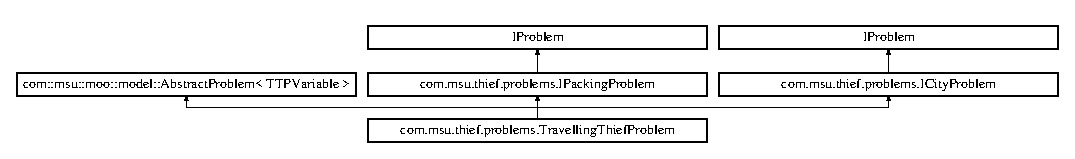
\includegraphics[height=1.686747cm]{classcom_1_1msu_1_1thief_1_1problems_1_1TravellingThiefProblem}
\end{center}
\end{figure}
\subsection*{Public Member Functions}
\begin{DoxyCompactItemize}
\item 
\hypertarget{classcom_1_1msu_1_1thief_1_1problems_1_1TravellingThiefProblem_a9242932977760ed10b2ea32a6c85c416}{{\bfseries Travelling\-Thief\-Problem} (\hyperlink{classcom_1_1msu_1_1thief_1_1model_1_1SymmetricMap}{Symmetric\-Map} map, Item\-Collection$<$ \hyperlink{classcom_1_1msu_1_1thief_1_1model_1_1Item}{Item} $>$ items, int max\-Weight)}\label{classcom_1_1msu_1_1thief_1_1problems_1_1TravellingThiefProblem_a9242932977760ed10b2ea32a6c85c416}

\item 
\hypertarget{classcom_1_1msu_1_1thief_1_1problems_1_1TravellingThiefProblem_a77375502664d11a35b61fdb837cc0070}{int {\bfseries num\-Of\-Cities} ()}\label{classcom_1_1msu_1_1thief_1_1problems_1_1TravellingThiefProblem_a77375502664d11a35b61fdb837cc0070}

\item 
\hypertarget{classcom_1_1msu_1_1thief_1_1problems_1_1TravellingThiefProblem_aa5bb95de358dbc9ca3bb1286984002dd}{int {\bfseries num\-Of\-Items} ()}\label{classcom_1_1msu_1_1thief_1_1problems_1_1TravellingThiefProblem_aa5bb95de358dbc9ca3bb1286984002dd}

\item 
\hypertarget{classcom_1_1msu_1_1thief_1_1problems_1_1TravellingThiefProblem_acc8c93330182f1b15b2dac8e355bcae6}{int {\bfseries get\-Number\-Of\-Objectives} ()}\label{classcom_1_1msu_1_1thief_1_1problems_1_1TravellingThiefProblem_acc8c93330182f1b15b2dac8e355bcae6}

\item 
\hypertarget{classcom_1_1msu_1_1thief_1_1problems_1_1TravellingThiefProblem_a2dac28a7f53eb6629a2e885d15165bf4}{String {\bfseries to\-String} ()}\label{classcom_1_1msu_1_1thief_1_1problems_1_1TravellingThiefProblem_a2dac28a7f53eb6629a2e885d15165bf4}

\item 
\hypertarget{classcom_1_1msu_1_1thief_1_1problems_1_1TravellingThiefProblem_abeb4a59b078a87d854767f3c5ab6f16a}{void {\bfseries set\-Name} (String name)}\label{classcom_1_1msu_1_1thief_1_1problems_1_1TravellingThiefProblem_abeb4a59b078a87d854767f3c5ab6f16a}

\item 
\hypertarget{classcom_1_1msu_1_1thief_1_1problems_1_1TravellingThiefProblem_aae7bc4d0f3eca1b0567fc8d37fe602db}{\hyperlink{classcom_1_1msu_1_1thief_1_1model_1_1SymmetricMap}{Symmetric\-Map} {\bfseries get\-Map} ()}\label{classcom_1_1msu_1_1thief_1_1problems_1_1TravellingThiefProblem_aae7bc4d0f3eca1b0567fc8d37fe602db}

\item 
\hypertarget{classcom_1_1msu_1_1thief_1_1problems_1_1TravellingThiefProblem_a44f5613eaf034264e36dc4129d0232dc}{void {\bfseries set\-Map} (\hyperlink{classcom_1_1msu_1_1thief_1_1model_1_1SymmetricMap}{Symmetric\-Map} map)}\label{classcom_1_1msu_1_1thief_1_1problems_1_1TravellingThiefProblem_a44f5613eaf034264e36dc4129d0232dc}

\item 
\hypertarget{classcom_1_1msu_1_1thief_1_1problems_1_1TravellingThiefProblem_ae906d444ddb76999c82f81fec7938969}{int {\bfseries get\-Max\-Weight} ()}\label{classcom_1_1msu_1_1thief_1_1problems_1_1TravellingThiefProblem_ae906d444ddb76999c82f81fec7938969}

\item 
\hypertarget{classcom_1_1msu_1_1thief_1_1problems_1_1TravellingThiefProblem_ac43622c927ccc41c45e338c12b5b1687}{void {\bfseries set\-Max\-Weight} (int max\-Weight)}\label{classcom_1_1msu_1_1thief_1_1problems_1_1TravellingThiefProblem_ac43622c927ccc41c45e338c12b5b1687}

\item 
\hypertarget{classcom_1_1msu_1_1thief_1_1problems_1_1TravellingThiefProblem_a1997c138329e08b0ef8105da645bfe89}{Item\-Collection$<$ \hyperlink{classcom_1_1msu_1_1thief_1_1model_1_1Item}{Item} $>$ {\bfseries get\-Items} ()}\label{classcom_1_1msu_1_1thief_1_1problems_1_1TravellingThiefProblem_a1997c138329e08b0ef8105da645bfe89}

\item 
\hypertarget{classcom_1_1msu_1_1thief_1_1problems_1_1TravellingThiefProblem_ad6641cb95fb3d1c7ddc3fa50e8451f44}{void {\bfseries set\-Items} (Item\-Collection$<$ \hyperlink{classcom_1_1msu_1_1thief_1_1model_1_1Item}{Item} $>$ items)}\label{classcom_1_1msu_1_1thief_1_1problems_1_1TravellingThiefProblem_ad6641cb95fb3d1c7ddc3fa50e8451f44}

\item 
\hypertarget{classcom_1_1msu_1_1thief_1_1problems_1_1TravellingThiefProblem_a6eaeef17ab3f63735437604757437831}{\hyperlink{classcom_1_1msu_1_1thief_1_1evaluator_1_1profit_1_1ProfitEvaluator}{Profit\-Evaluator} {\bfseries get\-Profit\-Evaluator} ()}\label{classcom_1_1msu_1_1thief_1_1problems_1_1TravellingThiefProblem_a6eaeef17ab3f63735437604757437831}

\item 
\hypertarget{classcom_1_1msu_1_1thief_1_1problems_1_1TravellingThiefProblem_a30dbaef6a3953033678351800cad4a98}{void {\bfseries set\-Profit\-Evaluator} (\hyperlink{classcom_1_1msu_1_1thief_1_1evaluator_1_1profit_1_1ProfitEvaluator}{Profit\-Evaluator} eval\-Profit)}\label{classcom_1_1msu_1_1thief_1_1problems_1_1TravellingThiefProblem_a30dbaef6a3953033678351800cad4a98}

\item 
\hypertarget{classcom_1_1msu_1_1thief_1_1problems_1_1TravellingThiefProblem_ace4b2b068d389c2a1e2e2ee7048f2afb}{\hyperlink{classcom_1_1msu_1_1thief_1_1evaluator_1_1time_1_1TimeEvaluator}{Time\-Evaluator} {\bfseries get\-Time\-Evaluator} ()}\label{classcom_1_1msu_1_1thief_1_1problems_1_1TravellingThiefProblem_ace4b2b068d389c2a1e2e2ee7048f2afb}

\item 
\hypertarget{classcom_1_1msu_1_1thief_1_1problems_1_1TravellingThiefProblem_ab19855b23101d8fede9886f27f7e627e}{void {\bfseries set\-Time\-Evaluator} (\hyperlink{classcom_1_1msu_1_1thief_1_1evaluator_1_1time_1_1TimeEvaluator}{Time\-Evaluator} eval\-Time)}\label{classcom_1_1msu_1_1thief_1_1problems_1_1TravellingThiefProblem_ab19855b23101d8fede9886f27f7e627e}

\item 
\hypertarget{classcom_1_1msu_1_1thief_1_1problems_1_1TravellingThiefProblem_a9ee842de681ed612d7b379de7cf255bf}{double {\bfseries get\-Min\-Speed} ()}\label{classcom_1_1msu_1_1thief_1_1problems_1_1TravellingThiefProblem_a9ee842de681ed612d7b379de7cf255bf}

\item 
\hypertarget{classcom_1_1msu_1_1thief_1_1problems_1_1TravellingThiefProblem_a4cfe39cc975134a3266167622dc4c614}{void {\bfseries set\-Min\-Speed} (double min\-Speed)}\label{classcom_1_1msu_1_1thief_1_1problems_1_1TravellingThiefProblem_a4cfe39cc975134a3266167622dc4c614}

\item 
\hypertarget{classcom_1_1msu_1_1thief_1_1problems_1_1TravellingThiefProblem_a349a07ec935f71f271630d27a896ee2a}{double {\bfseries get\-Max\-Speed} ()}\label{classcom_1_1msu_1_1thief_1_1problems_1_1TravellingThiefProblem_a349a07ec935f71f271630d27a896ee2a}

\item 
\hypertarget{classcom_1_1msu_1_1thief_1_1problems_1_1TravellingThiefProblem_a3ee35677936345b8d1fcda3cd7c36e5e}{void {\bfseries set\-Max\-Speed} (double max\-Speed)}\label{classcom_1_1msu_1_1thief_1_1problems_1_1TravellingThiefProblem_a3ee35677936345b8d1fcda3cd7c36e5e}

\end{DoxyCompactItemize}
\subsection*{Protected Member Functions}
\begin{DoxyCompactItemize}
\item 
\hypertarget{classcom_1_1msu_1_1thief_1_1problems_1_1TravellingThiefProblem_a8884c0f93a21c28b6c46c1401b8913b2}{List$<$ Double $>$ {\bfseries evaluate\-\_\-} (\hyperlink{classcom_1_1msu_1_1thief_1_1variable_1_1TTPVariable}{T\-T\-P\-Variable} variable)}\label{classcom_1_1msu_1_1thief_1_1problems_1_1TravellingThiefProblem_a8884c0f93a21c28b6c46c1401b8913b2}

\end{DoxyCompactItemize}
\subsection*{Protected Attributes}
\begin{DoxyCompactItemize}
\item 
\hypertarget{classcom_1_1msu_1_1thief_1_1problems_1_1TravellingThiefProblem_a2cdd4a9829b73f0c4eb22cac5480328a}{double {\bfseries min\-Speed} = 0.\-1d}\label{classcom_1_1msu_1_1thief_1_1problems_1_1TravellingThiefProblem_a2cdd4a9829b73f0c4eb22cac5480328a}

\item 
\hypertarget{classcom_1_1msu_1_1thief_1_1problems_1_1TravellingThiefProblem_abc30f65a025bd4893728acac9564b8df}{double {\bfseries max\-Speed} = 1.\-0d}\label{classcom_1_1msu_1_1thief_1_1problems_1_1TravellingThiefProblem_abc30f65a025bd4893728acac9564b8df}

\item 
\hypertarget{classcom_1_1msu_1_1thief_1_1problems_1_1TravellingThiefProblem_a636f5d9e02df73836963f5afa6393c62}{\hyperlink{classcom_1_1msu_1_1thief_1_1evaluator_1_1profit_1_1ProfitEvaluator}{Profit\-Evaluator} {\bfseries eval\-Profit} = new \hyperlink{classcom_1_1msu_1_1thief_1_1evaluator_1_1profit_1_1IndividualProfitEvaluator}{Individual\-Profit\-Evaluator}()}\label{classcom_1_1msu_1_1thief_1_1problems_1_1TravellingThiefProblem_a636f5d9e02df73836963f5afa6393c62}

\item 
\hypertarget{classcom_1_1msu_1_1thief_1_1problems_1_1TravellingThiefProblem_acee2627fdba072d2f50b9dd38f84a077}{\hyperlink{classcom_1_1msu_1_1thief_1_1evaluator_1_1time_1_1TimeEvaluator}{Time\-Evaluator} {\bfseries eval\-Time} = new \hyperlink{classcom_1_1msu_1_1thief_1_1evaluator_1_1time_1_1StandardTimeEvaluator}{Standard\-Time\-Evaluator}(this)}\label{classcom_1_1msu_1_1thief_1_1problems_1_1TravellingThiefProblem_acee2627fdba072d2f50b9dd38f84a077}

\item 
\hypertarget{classcom_1_1msu_1_1thief_1_1problems_1_1TravellingThiefProblem_a2a9abac0af7c09e43a9430f60aba3958}{String {\bfseries name} = \char`\"{}N\-O\-\_\-\-N\-A\-M\-E\char`\"{}}\label{classcom_1_1msu_1_1thief_1_1problems_1_1TravellingThiefProblem_a2a9abac0af7c09e43a9430f60aba3958}

\item 
\hypertarget{classcom_1_1msu_1_1thief_1_1problems_1_1TravellingThiefProblem_a499cd07177d6757a8e697b5d36bf642e}{\hyperlink{classcom_1_1msu_1_1thief_1_1model_1_1SymmetricMap}{Symmetric\-Map} {\bfseries map} = null}\label{classcom_1_1msu_1_1thief_1_1problems_1_1TravellingThiefProblem_a499cd07177d6757a8e697b5d36bf642e}

\item 
\hypertarget{classcom_1_1msu_1_1thief_1_1problems_1_1TravellingThiefProblem_af0354eb7a63a60f9d0a5dd4a092d8729}{int {\bfseries max\-Weight}}\label{classcom_1_1msu_1_1thief_1_1problems_1_1TravellingThiefProblem_af0354eb7a63a60f9d0a5dd4a092d8729}

\item 
\hypertarget{classcom_1_1msu_1_1thief_1_1problems_1_1TravellingThiefProblem_a1285ed72a98b9037a92358c1bfc4c9f8}{Item\-Collection$<$ \hyperlink{classcom_1_1msu_1_1thief_1_1model_1_1Item}{Item} $>$ {\bfseries items}}\label{classcom_1_1msu_1_1thief_1_1problems_1_1TravellingThiefProblem_a1285ed72a98b9037a92358c1bfc4c9f8}

\end{DoxyCompactItemize}


The documentation for this class was generated from the following file\-:\begin{DoxyCompactItemize}
\item 
src/main/java/com/msu/thief/problems/Travelling\-Thief\-Problem.\-java\end{DoxyCompactItemize}

\hypertarget{classcom_1_1msu_1_1tsp_1_1TSPExhaustiveFactory}{\section{com.\-msu.\-tsp.\-T\-S\-P\-Exhaustive\-Factory Class Reference}
\label{classcom_1_1msu_1_1tsp_1_1TSPExhaustiveFactory}\index{com.\-msu.\-tsp.\-T\-S\-P\-Exhaustive\-Factory@{com.\-msu.\-tsp.\-T\-S\-P\-Exhaustive\-Factory}}
}
Inheritance diagram for com.\-msu.\-tsp.\-T\-S\-P\-Exhaustive\-Factory\-:\begin{figure}[H]
\begin{center}
\leavevmode
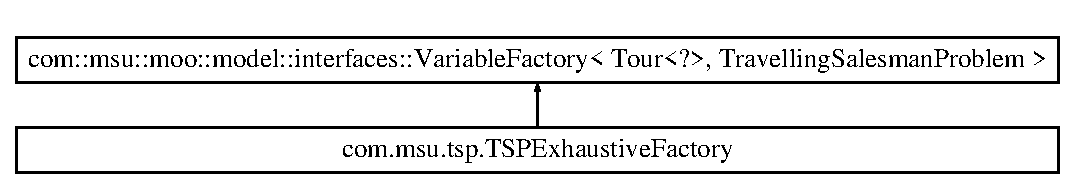
\includegraphics[height=2.000000cm]{classcom_1_1msu_1_1tsp_1_1TSPExhaustiveFactory}
\end{center}
\end{figure}
\subsection*{Public Member Functions}
\begin{DoxyCompactItemize}
\item 
\hypertarget{classcom_1_1msu_1_1tsp_1_1TSPExhaustiveFactory_ad288064f0d4a6615eae0cb1e870f571a}{Tour$<$?$>$ {\bfseries create} (\hyperlink{classcom_1_1msu_1_1tsp_1_1TravellingSalesmanProblem}{Travelling\-Salesman\-Problem} problem)}\label{classcom_1_1msu_1_1tsp_1_1TSPExhaustiveFactory_ad288064f0d4a6615eae0cb1e870f571a}

\end{DoxyCompactItemize}
\subsection*{Protected Attributes}
\begin{DoxyCompactItemize}
\item 
\hypertarget{classcom_1_1msu_1_1tsp_1_1TSPExhaustiveFactory_aca52802a2fab96853892e8b0a83df1bb}{Queue$<$ List$<$ Integer $>$ $>$ \hyperlink{classcom_1_1msu_1_1tsp_1_1TSPExhaustiveFactory_aca52802a2fab96853892e8b0a83df1bb}{permutations} = null}\label{classcom_1_1msu_1_1tsp_1_1TSPExhaustiveFactory_aca52802a2fab96853892e8b0a83df1bb}

\begin{DoxyCompactList}\small\item\em all the permutations that exist \end{DoxyCompactList}\end{DoxyCompactItemize}


The documentation for this class was generated from the following file\-:\begin{DoxyCompactItemize}
\item 
src/main/java/com/msu/tsp/T\-S\-P\-Exhaustive\-Factory.\-java\end{DoxyCompactItemize}

\hypertarget{classcom_1_1msu_1_1thief_1_1experiment_1_1TSPOperatorExperiment}{\section{com.\-msu.\-thief.\-experiment.\-T\-S\-P\-Operator\-Experiment Class Reference}
\label{classcom_1_1msu_1_1thief_1_1experiment_1_1TSPOperatorExperiment}\index{com.\-msu.\-thief.\-experiment.\-T\-S\-P\-Operator\-Experiment@{com.\-msu.\-thief.\-experiment.\-T\-S\-P\-Operator\-Experiment}}
}
Inheritance diagram for com.\-msu.\-thief.\-experiment.\-T\-S\-P\-Operator\-Experiment\-:\begin{figure}[H]
\begin{center}
\leavevmode
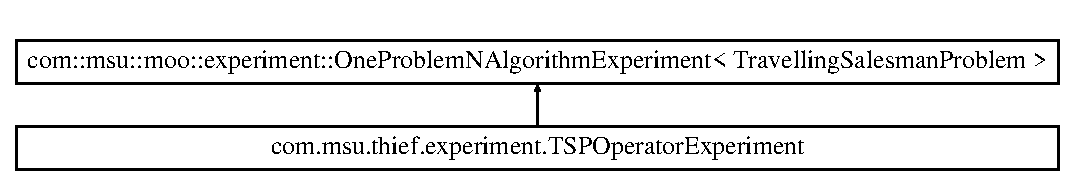
\includegraphics[height=2.000000cm]{classcom_1_1msu_1_1thief_1_1experiment_1_1TSPOperatorExperiment}
\end{center}
\end{figure}
\subsection*{Public Member Functions}
\begin{DoxyCompactItemize}
\item 
\hypertarget{classcom_1_1msu_1_1thief_1_1experiment_1_1TSPOperatorExperiment_a7a38886831cd2f89cac6baa22c9d5683}{void {\bfseries report} ()}\label{classcom_1_1msu_1_1thief_1_1experiment_1_1TSPOperatorExperiment_a7a38886831cd2f89cac6baa22c9d5683}

\end{DoxyCompactItemize}
\subsection*{Static Public Member Functions}
\begin{DoxyCompactItemize}
\item 
\hypertarget{classcom_1_1msu_1_1thief_1_1experiment_1_1TSPOperatorExperiment_a7016b060abe4c7124a5bf6b185e9c0cb}{static void {\bfseries main} (String\mbox{[}$\,$\mbox{]} args)}\label{classcom_1_1msu_1_1thief_1_1experiment_1_1TSPOperatorExperiment_a7016b060abe4c7124a5bf6b185e9c0cb}

\end{DoxyCompactItemize}
\subsection*{Protected Member Functions}
\begin{DoxyCompactItemize}
\item 
\hypertarget{classcom_1_1msu_1_1thief_1_1experiment_1_1TSPOperatorExperiment_a7e970c51a378d6e1c9d4a36bc815afe9}{List$<$ I\-Algorithm\\*
$<$ \hyperlink{classcom_1_1msu_1_1tsp_1_1TravellingSalesmanProblem}{Travelling\-Salesman\-Problem} $>$ $>$ {\bfseries get\-Algorithms} ()}\label{classcom_1_1msu_1_1thief_1_1experiment_1_1TSPOperatorExperiment_a7e970c51a378d6e1c9d4a36bc815afe9}

\item 
\hypertarget{classcom_1_1msu_1_1thief_1_1experiment_1_1TSPOperatorExperiment_af0ccec33727502527d72e691c3d53b5a}{\hyperlink{classcom_1_1msu_1_1tsp_1_1TravellingSalesmanProblem}{Travelling\-Salesman\-Problem} {\bfseries get\-Problem} ()}\label{classcom_1_1msu_1_1thief_1_1experiment_1_1TSPOperatorExperiment_af0ccec33727502527d72e691c3d53b5a}

\item 
\hypertarget{classcom_1_1msu_1_1thief_1_1experiment_1_1TSPOperatorExperiment_aa197dc736547d3d1bd0239a23ba3145c}{Non\-Dominated\-Solution\-Set {\bfseries get\-True\-Front} ()}\label{classcom_1_1msu_1_1thief_1_1experiment_1_1TSPOperatorExperiment_aa197dc736547d3d1bd0239a23ba3145c}

\end{DoxyCompactItemize}


The documentation for this class was generated from the following file\-:\begin{DoxyCompactItemize}
\item 
src/main/java/com/msu/thief/experiment/T\-S\-P\-Operator\-Experiment.\-java\end{DoxyCompactItemize}

\hypertarget{classcom_1_1msu_1_1thief_1_1variable_1_1TTPCrossover}{\section{com.\-msu.\-thief.\-variable.\-T\-T\-P\-Crossover Class Reference}
\label{classcom_1_1msu_1_1thief_1_1variable_1_1TTPCrossover}\index{com.\-msu.\-thief.\-variable.\-T\-T\-P\-Crossover@{com.\-msu.\-thief.\-variable.\-T\-T\-P\-Crossover}}
}
Inheritance diagram for com.\-msu.\-thief.\-variable.\-T\-T\-P\-Crossover\-:\begin{figure}[H]
\begin{center}
\leavevmode
\includegraphics[height=2.000000cm]{classcom_1_1msu_1_1thief_1_1variable_1_1TTPCrossover}
\end{center}
\end{figure}
\subsection*{Public Member Functions}
\begin{DoxyCompactItemize}
\item 
\hypertarget{classcom_1_1msu_1_1thief_1_1variable_1_1TTPCrossover_aeadae4cc69d473615b388657dd482c90}{{\bfseries T\-T\-P\-Crossover} (Abstract\-Crossover$<$?$>$ \hyperlink{classcom_1_1msu_1_1thief_1_1variable_1_1TTPCrossover_a392a724cbf3c5e88e2648adcfd17f02f}{c\-Tour}, Abstract\-Crossover$<$?$>$ \hyperlink{classcom_1_1msu_1_1thief_1_1variable_1_1TTPCrossover_a65c9d474482814cdc26a896c3377e160}{c\-Packing\-Plan})}\label{classcom_1_1msu_1_1thief_1_1variable_1_1TTPCrossover_aeadae4cc69d473615b388657dd482c90}

\end{DoxyCompactItemize}
\subsection*{Protected Member Functions}
\begin{DoxyCompactItemize}
\item 
\hypertarget{classcom_1_1msu_1_1thief_1_1variable_1_1TTPCrossover_ad94acfeb50ec5590f5b797fe702382d3}{List$<$ Pair$<$ I\-Variable, \\*
I\-Variable $>$ $>$ {\bfseries crossover\-\_\-} (Pair$<$ I\-Variable, I\-Variable $>$ a, Pair$<$ I\-Variable, I\-Variable $>$ b)}\label{classcom_1_1msu_1_1thief_1_1variable_1_1TTPCrossover_ad94acfeb50ec5590f5b797fe702382d3}

\end{DoxyCompactItemize}
\subsection*{Protected Attributes}
\begin{DoxyCompactItemize}
\item 
\hypertarget{classcom_1_1msu_1_1thief_1_1variable_1_1TTPCrossover_a392a724cbf3c5e88e2648adcfd17f02f}{Abstract\-Crossover$<$?$>$ \hyperlink{classcom_1_1msu_1_1thief_1_1variable_1_1TTPCrossover_a392a724cbf3c5e88e2648adcfd17f02f}{c\-Tour}}\label{classcom_1_1msu_1_1thief_1_1variable_1_1TTPCrossover_a392a724cbf3c5e88e2648adcfd17f02f}

\begin{DoxyCompactList}\small\item\em crossover for the tour \end{DoxyCompactList}\item 
\hypertarget{classcom_1_1msu_1_1thief_1_1variable_1_1TTPCrossover_a65c9d474482814cdc26a896c3377e160}{Abstract\-Crossover$<$?$>$ \hyperlink{classcom_1_1msu_1_1thief_1_1variable_1_1TTPCrossover_a65c9d474482814cdc26a896c3377e160}{c\-Packing\-Plan}}\label{classcom_1_1msu_1_1thief_1_1variable_1_1TTPCrossover_a65c9d474482814cdc26a896c3377e160}

\begin{DoxyCompactList}\small\item\em crossover for the packing plan \end{DoxyCompactList}\end{DoxyCompactItemize}


The documentation for this class was generated from the following file\-:\begin{DoxyCompactItemize}
\item 
src/main/java/com/msu/thief/variable/T\-T\-P\-Crossover.\-java\end{DoxyCompactItemize}

\hypertarget{classcom_1_1msu_1_1thief_1_1problems_1_1TTPExhaustiveFactory}{\section{com.\-msu.\-thief.\-problems.\-T\-T\-P\-Exhaustive\-Factory Class Reference}
\label{classcom_1_1msu_1_1thief_1_1problems_1_1TTPExhaustiveFactory}\index{com.\-msu.\-thief.\-problems.\-T\-T\-P\-Exhaustive\-Factory@{com.\-msu.\-thief.\-problems.\-T\-T\-P\-Exhaustive\-Factory}}
}
Inheritance diagram for com.\-msu.\-thief.\-problems.\-T\-T\-P\-Exhaustive\-Factory\-:\begin{figure}[H]
\begin{center}
\leavevmode
\includegraphics[height=2.000000cm]{classcom_1_1msu_1_1thief_1_1problems_1_1TTPExhaustiveFactory}
\end{center}
\end{figure}
\subsection*{Public Member Functions}
\begin{DoxyCompactItemize}
\item 
\hypertarget{classcom_1_1msu_1_1thief_1_1problems_1_1TTPExhaustiveFactory_a831d81cded0de2536f45611061d85503}{\hyperlink{classcom_1_1msu_1_1thief_1_1variable_1_1TTPVariable}{T\-T\-P\-Variable} {\bfseries create} (\hyperlink{classcom_1_1msu_1_1thief_1_1problems_1_1TravellingThiefProblem}{Travelling\-Thief\-Problem} problem)}\label{classcom_1_1msu_1_1thief_1_1problems_1_1TTPExhaustiveFactory_a831d81cded0de2536f45611061d85503}

\end{DoxyCompactItemize}
\subsection*{Protected Attributes}
\begin{DoxyCompactItemize}
\item 
\hypertarget{classcom_1_1msu_1_1thief_1_1problems_1_1TTPExhaustiveFactory_ab950e5d6fec07671c9306c467816c946}{Queue$<$ \hyperlink{classcom_1_1msu_1_1thief_1_1variable_1_1TTPVariable}{T\-T\-P\-Variable} $>$ \hyperlink{classcom_1_1msu_1_1thief_1_1problems_1_1TTPExhaustiveFactory_ab950e5d6fec07671c9306c467816c946}{Q} = null}\label{classcom_1_1msu_1_1thief_1_1problems_1_1TTPExhaustiveFactory_ab950e5d6fec07671c9306c467816c946}

\begin{DoxyCompactList}\small\item\em all the permutations that exist \end{DoxyCompactList}\item 
\hypertarget{classcom_1_1msu_1_1thief_1_1problems_1_1TTPExhaustiveFactory_a1bb8f5a0cb4a48b603dd605290ed551f}{\hyperlink{classcom_1_1msu_1_1tsp_1_1TSPExhaustiveFactory}{T\-S\-P\-Exhaustive\-Factory} {\bfseries fac\-T\-S\-P} = new \hyperlink{classcom_1_1msu_1_1tsp_1_1TSPExhaustiveFactory}{T\-S\-P\-Exhaustive\-Factory}()}\label{classcom_1_1msu_1_1thief_1_1problems_1_1TTPExhaustiveFactory_a1bb8f5a0cb4a48b603dd605290ed551f}

\item 
\hypertarget{classcom_1_1msu_1_1thief_1_1problems_1_1TTPExhaustiveFactory_a368a3c57843610d488183ef7183f98fd}{\hyperlink{classcom_1_1msu_1_1knp_1_1KnapsackExhaustiveFactory}{Knapsack\-Exhaustive\-Factory} {\bfseries fac\-K\-N\-P} = new \hyperlink{classcom_1_1msu_1_1knp_1_1KnapsackExhaustiveFactory}{Knapsack\-Exhaustive\-Factory}()}\label{classcom_1_1msu_1_1thief_1_1problems_1_1TTPExhaustiveFactory_a368a3c57843610d488183ef7183f98fd}

\end{DoxyCompactItemize}


The documentation for this class was generated from the following file\-:\begin{DoxyCompactItemize}
\item 
src/main/java/com/msu/thief/problems/T\-T\-P\-Exhaustive\-Factory.\-java\end{DoxyCompactItemize}

\hypertarget{classcom_1_1msu_1_1thief_1_1variable_1_1TTPMutation}{\section{com.\-msu.\-thief.\-variable.\-T\-T\-P\-Mutation Class Reference}
\label{classcom_1_1msu_1_1thief_1_1variable_1_1TTPMutation}\index{com.\-msu.\-thief.\-variable.\-T\-T\-P\-Mutation@{com.\-msu.\-thief.\-variable.\-T\-T\-P\-Mutation}}
}
Inheritance diagram for com.\-msu.\-thief.\-variable.\-T\-T\-P\-Mutation\-:\begin{figure}[H]
\begin{center}
\leavevmode
\includegraphics[height=2.000000cm]{classcom_1_1msu_1_1thief_1_1variable_1_1TTPMutation}
\end{center}
\end{figure}
\subsection*{Public Member Functions}
\begin{DoxyCompactItemize}
\item 
\hypertarget{classcom_1_1msu_1_1thief_1_1variable_1_1TTPMutation_a65b0b0ee53ca57500f2f270b0478f6d5}{{\bfseries T\-T\-P\-Mutation} (Abstract\-Mutation$<$?$>$ \hyperlink{classcom_1_1msu_1_1thief_1_1variable_1_1TTPMutation_ace8bf1825ff37a4e0a4bdfa1ac581924}{m\-Tour}, Abstract\-Mutation$<$?$>$ \hyperlink{classcom_1_1msu_1_1thief_1_1variable_1_1TTPMutation_ad49e8ad884aad46fdc8724fd1e168f64}{m\-Packing\-Plan})}\label{classcom_1_1msu_1_1thief_1_1variable_1_1TTPMutation_a65b0b0ee53ca57500f2f270b0478f6d5}

\end{DoxyCompactItemize}
\subsection*{Protected Member Functions}
\begin{DoxyCompactItemize}
\item 
\hypertarget{classcom_1_1msu_1_1thief_1_1variable_1_1TTPMutation_a1f50962a59474c475247d80a2940112b}{void {\bfseries mutate\-\_\-} (Pair$<$ I\-Variable, I\-Variable $>$ a)}\label{classcom_1_1msu_1_1thief_1_1variable_1_1TTPMutation_a1f50962a59474c475247d80a2940112b}

\end{DoxyCompactItemize}
\subsection*{Protected Attributes}
\begin{DoxyCompactItemize}
\item 
\hypertarget{classcom_1_1msu_1_1thief_1_1variable_1_1TTPMutation_ace8bf1825ff37a4e0a4bdfa1ac581924}{Abstract\-Mutation$<$?$>$ \hyperlink{classcom_1_1msu_1_1thief_1_1variable_1_1TTPMutation_ace8bf1825ff37a4e0a4bdfa1ac581924}{m\-Tour}}\label{classcom_1_1msu_1_1thief_1_1variable_1_1TTPMutation_ace8bf1825ff37a4e0a4bdfa1ac581924}

\begin{DoxyCompactList}\small\item\em crossover for the tour \end{DoxyCompactList}\item 
\hypertarget{classcom_1_1msu_1_1thief_1_1variable_1_1TTPMutation_ad49e8ad884aad46fdc8724fd1e168f64}{Abstract\-Mutation$<$?$>$ \hyperlink{classcom_1_1msu_1_1thief_1_1variable_1_1TTPMutation_ad49e8ad884aad46fdc8724fd1e168f64}{m\-Packing\-Plan}}\label{classcom_1_1msu_1_1thief_1_1variable_1_1TTPMutation_ad49e8ad884aad46fdc8724fd1e168f64}

\begin{DoxyCompactList}\small\item\em crossover for the packing plan \end{DoxyCompactList}\end{DoxyCompactItemize}


The documentation for this class was generated from the following file\-:\begin{DoxyCompactItemize}
\item 
src/main/java/com/msu/thief/variable/T\-T\-P\-Mutation.\-java\end{DoxyCompactItemize}

\hypertarget{classcom_1_1msu_1_1thief_1_1variable_1_1TTPVariable}{\section{com.\-msu.\-thief.\-variable.\-T\-T\-P\-Variable Class Reference}
\label{classcom_1_1msu_1_1thief_1_1variable_1_1TTPVariable}\index{com.\-msu.\-thief.\-variable.\-T\-T\-P\-Variable@{com.\-msu.\-thief.\-variable.\-T\-T\-P\-Variable}}
}
Inheritance diagram for com.\-msu.\-thief.\-variable.\-T\-T\-P\-Variable\-:\begin{figure}[H]
\begin{center}
\leavevmode
\includegraphics[height=2.000000cm]{classcom_1_1msu_1_1thief_1_1variable_1_1TTPVariable}
\end{center}
\end{figure}
\subsection*{Public Member Functions}
\begin{DoxyCompactItemize}
\item 
\hypertarget{classcom_1_1msu_1_1thief_1_1variable_1_1TTPVariable_a3c8e564e6b9cf68a6cfb31de312634b7}{{\bfseries T\-T\-P\-Variable} (Pair$<$ Tour$<$?$>$, Packing\-List$<$?$>$$>$ obj)}\label{classcom_1_1msu_1_1thief_1_1variable_1_1TTPVariable_a3c8e564e6b9cf68a6cfb31de312634b7}

\item 
\hypertarget{classcom_1_1msu_1_1thief_1_1variable_1_1TTPVariable_a0e76b83c7d46c269bed8e31f783c62ec}{String {\bfseries to\-String} ()}\label{classcom_1_1msu_1_1thief_1_1variable_1_1TTPVariable_a0e76b83c7d46c269bed8e31f783c62ec}

\item 
\hypertarget{classcom_1_1msu_1_1thief_1_1variable_1_1TTPVariable_a3763b6b0d91613fae9be56262c0b78dc}{I\-Variable {\bfseries copy} ()}\label{classcom_1_1msu_1_1thief_1_1variable_1_1TTPVariable_a3763b6b0d91613fae9be56262c0b78dc}

\end{DoxyCompactItemize}


The documentation for this class was generated from the following file\-:\begin{DoxyCompactItemize}
\item 
src/main/java/com/msu/thief/variable/T\-T\-P\-Variable.\-java\end{DoxyCompactItemize}

\hypertarget{classcom_1_1msu_1_1thief_1_1variable_1_1TTPVariableFactory}{\section{com.\-msu.\-thief.\-variable.\-T\-T\-P\-Variable\-Factory Class Reference}
\label{classcom_1_1msu_1_1thief_1_1variable_1_1TTPVariableFactory}\index{com.\-msu.\-thief.\-variable.\-T\-T\-P\-Variable\-Factory@{com.\-msu.\-thief.\-variable.\-T\-T\-P\-Variable\-Factory}}
}
Inheritance diagram for com.\-msu.\-thief.\-variable.\-T\-T\-P\-Variable\-Factory\-:\begin{figure}[H]
\begin{center}
\leavevmode
\includegraphics[height=2.000000cm]{classcom_1_1msu_1_1thief_1_1variable_1_1TTPVariableFactory}
\end{center}
\end{figure}
\subsection*{Public Member Functions}
\begin{DoxyCompactItemize}
\item 
\hypertarget{classcom_1_1msu_1_1thief_1_1variable_1_1TTPVariableFactory_a3c468c8106750307127d7710613429b6}{{\bfseries T\-T\-P\-Variable\-Factory} (I\-Tour\-Factory$<$ \hyperlink{classcom_1_1msu_1_1thief_1_1problems_1_1TravellingThiefProblem}{Travelling\-Thief\-Problem} $>$ fac\-Tour, \hyperlink{interfacecom_1_1msu_1_1thief_1_1model_1_1packing_1_1IPackingPlanFactory}{I\-Packing\-Plan\-Factory} fac\-Plan)}\label{classcom_1_1msu_1_1thief_1_1variable_1_1TTPVariableFactory_a3c468c8106750307127d7710613429b6}

\item 
\hypertarget{classcom_1_1msu_1_1thief_1_1variable_1_1TTPVariableFactory_a8af6b49ffdf1fe58ffc203f2f7f71e8e}{\hyperlink{classcom_1_1msu_1_1thief_1_1variable_1_1TTPVariable}{T\-T\-P\-Variable} {\bfseries create} (\hyperlink{classcom_1_1msu_1_1thief_1_1problems_1_1TravellingThiefProblem}{Travelling\-Thief\-Problem} problem)}\label{classcom_1_1msu_1_1thief_1_1variable_1_1TTPVariableFactory_a8af6b49ffdf1fe58ffc203f2f7f71e8e}

\end{DoxyCompactItemize}
\subsection*{Protected Attributes}
\begin{DoxyCompactItemize}
\item 
\hypertarget{classcom_1_1msu_1_1thief_1_1variable_1_1TTPVariableFactory_ad68bd9a1906cfe270ec71bec4814a544}{I\-Tour\-Factory\\*
$<$ \hyperlink{classcom_1_1msu_1_1thief_1_1problems_1_1TravellingThiefProblem}{Travelling\-Thief\-Problem} $>$ {\bfseries fac\-Tour}}\label{classcom_1_1msu_1_1thief_1_1variable_1_1TTPVariableFactory_ad68bd9a1906cfe270ec71bec4814a544}

\item 
\hypertarget{classcom_1_1msu_1_1thief_1_1variable_1_1TTPVariableFactory_adabbde28604cafa9727be18c8218114c}{\hyperlink{interfacecom_1_1msu_1_1thief_1_1model_1_1packing_1_1IPackingPlanFactory}{I\-Packing\-Plan\-Factory} {\bfseries fac\-Plan}}\label{classcom_1_1msu_1_1thief_1_1variable_1_1TTPVariableFactory_adabbde28604cafa9727be18c8218114c}

\end{DoxyCompactItemize}


The documentation for this class was generated from the following file\-:\begin{DoxyCompactItemize}
\item 
src/main/java/com/msu/thief/variable/T\-T\-P\-Variable\-Factory.\-java\end{DoxyCompactItemize}

\hypertarget{classcom_1_1msu_1_1thief_1_1util_1_1Util}{\section{com.\-msu.\-thief.\-util.\-Util Class Reference}
\label{classcom_1_1msu_1_1thief_1_1util_1_1Util}\index{com.\-msu.\-thief.\-util.\-Util@{com.\-msu.\-thief.\-util.\-Util}}
}
\subsection*{Static Public Member Functions}
\begin{DoxyCompactItemize}
\item 
static$<$ T $>$ T \hyperlink{classcom_1_1msu_1_1thief_1_1util_1_1Util_a0f13ff65d9c54adc3a743e912c73469d}{get\-Duplicate} (Hash\-Set$<$ T $>$ hash, Collection$<$ T $>$ c)
\end{DoxyCompactItemize}


\subsection{Member Function Documentation}
\hypertarget{classcom_1_1msu_1_1thief_1_1util_1_1Util_a0f13ff65d9c54adc3a743e912c73469d}{\index{com\-::msu\-::thief\-::util\-::\-Util@{com\-::msu\-::thief\-::util\-::\-Util}!get\-Duplicate@{get\-Duplicate}}
\index{get\-Duplicate@{get\-Duplicate}!com::msu::thief::util::Util@{com\-::msu\-::thief\-::util\-::\-Util}}
\subsubsection[{get\-Duplicate}]{\setlength{\rightskip}{0pt plus 5cm}static $<$T$>$ T com.\-msu.\-thief.\-util.\-Util.\-get\-Duplicate (
\begin{DoxyParamCaption}
\item[{Hash\-Set$<$ T $>$}]{hash, }
\item[{Collection$<$ T $>$}]{c}
\end{DoxyParamCaption}
)\hspace{0.3cm}{\ttfamily [inline]}, {\ttfamily [static]}}}\label{classcom_1_1msu_1_1thief_1_1util_1_1Util_a0f13ff65d9c54adc3a743e912c73469d}
Return the first duplicate that is found on a given collection 
\begin{DoxyParams}{Parameters}
{\em c} & collection of a generic type. \\
\hline
\end{DoxyParams}
\begin{DoxyReturn}{Returns}
first found duplicate 
\end{DoxyReturn}


The documentation for this class was generated from the following file\-:\begin{DoxyCompactItemize}
\item 
src/main/java/com/msu/thief/util/Util.\-java\end{DoxyCompactItemize}

%--- End generated contents ---

% Index
\newpage
\phantomsection
\addcontentsline{toc}{chapter}{Index}
\printindex

\end{document}
